% Options for packages loaded elsewhere
\PassOptionsToPackage{unicode}{hyperref}
\PassOptionsToPackage{hyphens}{url}
%
\documentclass[
]{book}
\usepackage{lmodern}
\usepackage{amssymb,amsmath}
\usepackage{ifxetex,ifluatex}
\ifnum 0\ifxetex 1\fi\ifluatex 1\fi=0 % if pdftex
  \usepackage[T1]{fontenc}
  \usepackage[utf8]{inputenc}
  \usepackage{textcomp} % provide euro and other symbols
\else % if luatex or xetex
  \usepackage{unicode-math}
  \defaultfontfeatures{Scale=MatchLowercase}
  \defaultfontfeatures[\rmfamily]{Ligatures=TeX,Scale=1}
\fi
% Use upquote if available, for straight quotes in verbatim environments
\IfFileExists{upquote.sty}{\usepackage{upquote}}{}
\IfFileExists{microtype.sty}{% use microtype if available
  \usepackage[]{microtype}
  \UseMicrotypeSet[protrusion]{basicmath} % disable protrusion for tt fonts
}{}
\makeatletter
\@ifundefined{KOMAClassName}{% if non-KOMA class
  \IfFileExists{parskip.sty}{%
    \usepackage{parskip}
  }{% else
    \setlength{\parindent}{0pt}
    \setlength{\parskip}{6pt plus 2pt minus 1pt}}
}{% if KOMA class
  \KOMAoptions{parskip=half}}
\makeatother
\usepackage{xcolor}
\IfFileExists{xurl.sty}{\usepackage{xurl}}{} % add URL line breaks if available
\IfFileExists{bookmark.sty}{\usepackage{bookmark}}{\usepackage{hyperref}}
\hypersetup{
  pdftitle={CH10137 Thermodynamics},
  pdfauthor={Fiona Dickinson},
  hidelinks,
  pdfcreator={LaTeX via pandoc}}
\urlstyle{same} % disable monospaced font for URLs
\usepackage{longtable,booktabs}
% Correct order of tables after \paragraph or \subparagraph
\usepackage{etoolbox}
\makeatletter
\patchcmd\longtable{\par}{\if@noskipsec\mbox{}\fi\par}{}{}
\makeatother
% Allow footnotes in longtable head/foot
\IfFileExists{footnotehyper.sty}{\usepackage{footnotehyper}}{\usepackage{footnote}}
\makesavenoteenv{longtable}
\usepackage{graphicx,grffile}
\makeatletter
\def\maxwidth{\ifdim\Gin@nat@width>\linewidth\linewidth\else\Gin@nat@width\fi}
\def\maxheight{\ifdim\Gin@nat@height>\textheight\textheight\else\Gin@nat@height\fi}
\makeatother
% Scale images if necessary, so that they will not overflow the page
% margins by default, and it is still possible to overwrite the defaults
% using explicit options in \includegraphics[width, height, ...]{}
\setkeys{Gin}{width=\maxwidth,height=\maxheight,keepaspectratio}
% Set default figure placement to htbp
\makeatletter
\def\fps@figure{htbp}
\makeatother
\setlength{\emergencystretch}{3em} % prevent overfull lines
\providecommand{\tightlist}{%
  \setlength{\itemsep}{0pt}\setlength{\parskip}{0pt}}
\setcounter{secnumdepth}{5}
\usepackage{booktabs}
\usepackage{amsthm}
\makeatletter
\def\thm@space@setup{%
  \thm@preskip=8pt plus 2pt minus 4pt
  \thm@postskip=\thm@preskip
}
\makeatother
\usepackage[]{natbib}
\bibliographystyle{apalike}

\title{CH10137 Thermodynamics}
\author{Fiona Dickinson}
\date{2021-11-19}

\begin{document}
\maketitle

{
\setcounter{tocdepth}{1}
\tableofcontents
}
\hypertarget{welcome}{%
\chapter*{Welcome}\label{welcome}}
\addcontentsline{toc}{chapter}{Welcome}

The notes have been prepared in a package called BookDown for RStudio so that the equations are accessible to screen readers. However, by providing the notes as a .html webpage I can also embed short videos to further describe some of the topics. If you want videos on any topic please ask and I will do my best to produce the most requested ones.

Further you can download the notes in a format that suits you (either pdf or epub) to view offline, or change the way this document appears for ease of reading.

This document is written in markdown, and particularly in equations typos can creep in. If you spot any typos or think there are any errors please let me know and I will do my best to fix them.

\hypertarget{notes-and-workshops-for-ch10137}{%
\section*{Notes and Workshops for CH10137}\label{notes-and-workshops-for-ch10137}}
\addcontentsline{toc}{section}{Notes and Workshops for CH10137}

This `book' will be updated weekly with content and embedded `micro lecture' video content.

Questions and answers will be provided and some answers will include `process' as well as answer. Please contact me if you need help. Questions on later topics will rely on earlier knowledge.

I am using this format as it is an accessible format. However I have moved over to this format this year and so I would appreciate you pointing out any areas of confusion or where error may have crept in.

\hypertarget{recommended-text}{%
\section*{Recommended text}\label{recommended-text}}
\addcontentsline{toc}{section}{Recommended text}

There is no single recommended text for this section of the course because multiple books can offer valuable extra insight. It may be useful for you to refer to any of the following:

\href{https://bath-ac-primo.hosted.exlibrisgroup.com/primo-explore/search?query=any,contains,Elements\%20of\%20physical\%20chemistry\&tab=local\&sortby=date\&vid=44BAT_VU1\&facet=frbrgroupid,include,978286819\&offset=0\&pcAvailability=false}{The Elements of Physical Chemistry}

\href{https://bath-ac-primo.hosted.exlibrisgroup.com/primo-explore/search?query=any,contains,physical\%20chemistry\%20de\%20paula\&tab=local\&search_scope=CSCOP_44BAT_DEEP\&sortby=date\&vid=44BAT_VU1\&facet=frbrgroupid,include,978327499\&offset=0\&pcAvailability=false}{Atkins' Physical Chemistry}

\href{https://bath-ac-primo.hosted.exlibrisgroup.com/primo-explore/search?query=any,contains,chemistry3\&tab=local\&search_scope=CSCOP_44BAT_DEEP\&sortby=date\&vid=44BAT_VU1\&facet=frbrgroupid,include,978293871\&offset=0\&pcAvailability=false}{Chemistry\textsuperscript{3}}

\hypertarget{report-errors}{%
\section*{Report errors}\label{report-errors}}
\addcontentsline{toc}{section}{Report errors}

If you spot any errors or areas of lack of clarity, please message me in Teams or preferably report on the error log below:

Loading\ldots{}

\hypertarget{version-history}{%
\section*{Version history}\label{version-history}}
\addcontentsline{toc}{section}{Version history}

Typos fixed 191121

21-22 version first commit 291021

Covid version finished 181120

The initial commit of this book is dated 16th October 2020.

\hypertarget{ch:Part1}{%
\chapter{Week 1 - Part 1: Preliminaries}\label{ch:Part1}}

The `content' videos are all very short, any equations or important images are contained in the text of this document and so pdf slides will not be shared (as these are not an accessible document).

\hypertarget{sec:whyjustwhy}{%
\section{Why thermodynamics matters}\label{sec:whyjustwhy}}

The laws of thermodynamics are some of the most fundamental laws of nature, and in this course I hope you will learn to understand these laws and be able to apply them to explain the world around you.

Thermodynamics is fundamental to the way we live, to our dream of living a better, less impactful life and to how we as `life' work.

\hypertarget{sec:state}{%
\section{State functions - (products - reactants)}\label{sec:state}}

Many properties in thermodynamics are \emph{state functions}, that is properties that only depend upon the current state of the system. State functions are completely independent of the path by which that final state was reached.

Enthalpy (\(H\)) is a state function, as are entropy (\(S\)), internal energy (\(U\)), Gibbs' free energy (\(G\)), Helmholtz free energy (\(F\)), temperature (\(T\)), pressure (\(p\)), and chemical composition.

Path functions are unlike state functions in that they depend on the path taken to determine their value.
Heat (\(q\)) and work (\(w\)) are both examples of path functions.

\begin{itemize}
\item
  \textbf{Internal energy,} \(U\) The internal energy is the sum of all of the kinetic and potential energy contributions of the molecules in the system.
\item
  \textbf{Enthalpy,} \(H\) The enthalpy is related to the internal energy, but also takes into account any expansion work done by the system, formally ΔH = ΔU + Δ(pV).
\item
  \textbf{Entropy,} \(S\) The entropy is a measure of the number of possible arrangements of a system (multiplicity, \(Ω\)), formally \(S = k_B \ln Ω\)
\item
  \textbf{Gibbs' free energy,} \(G\) The Gibbs' free energy is a measure of the energy available to `do work' in a reaction system. It accounts for both the enalpic and entropic contributions of the reaction. \(\Delta G = \Delta H − T \Delta S\)
\end{itemize}

\begin{figure}

{\centering 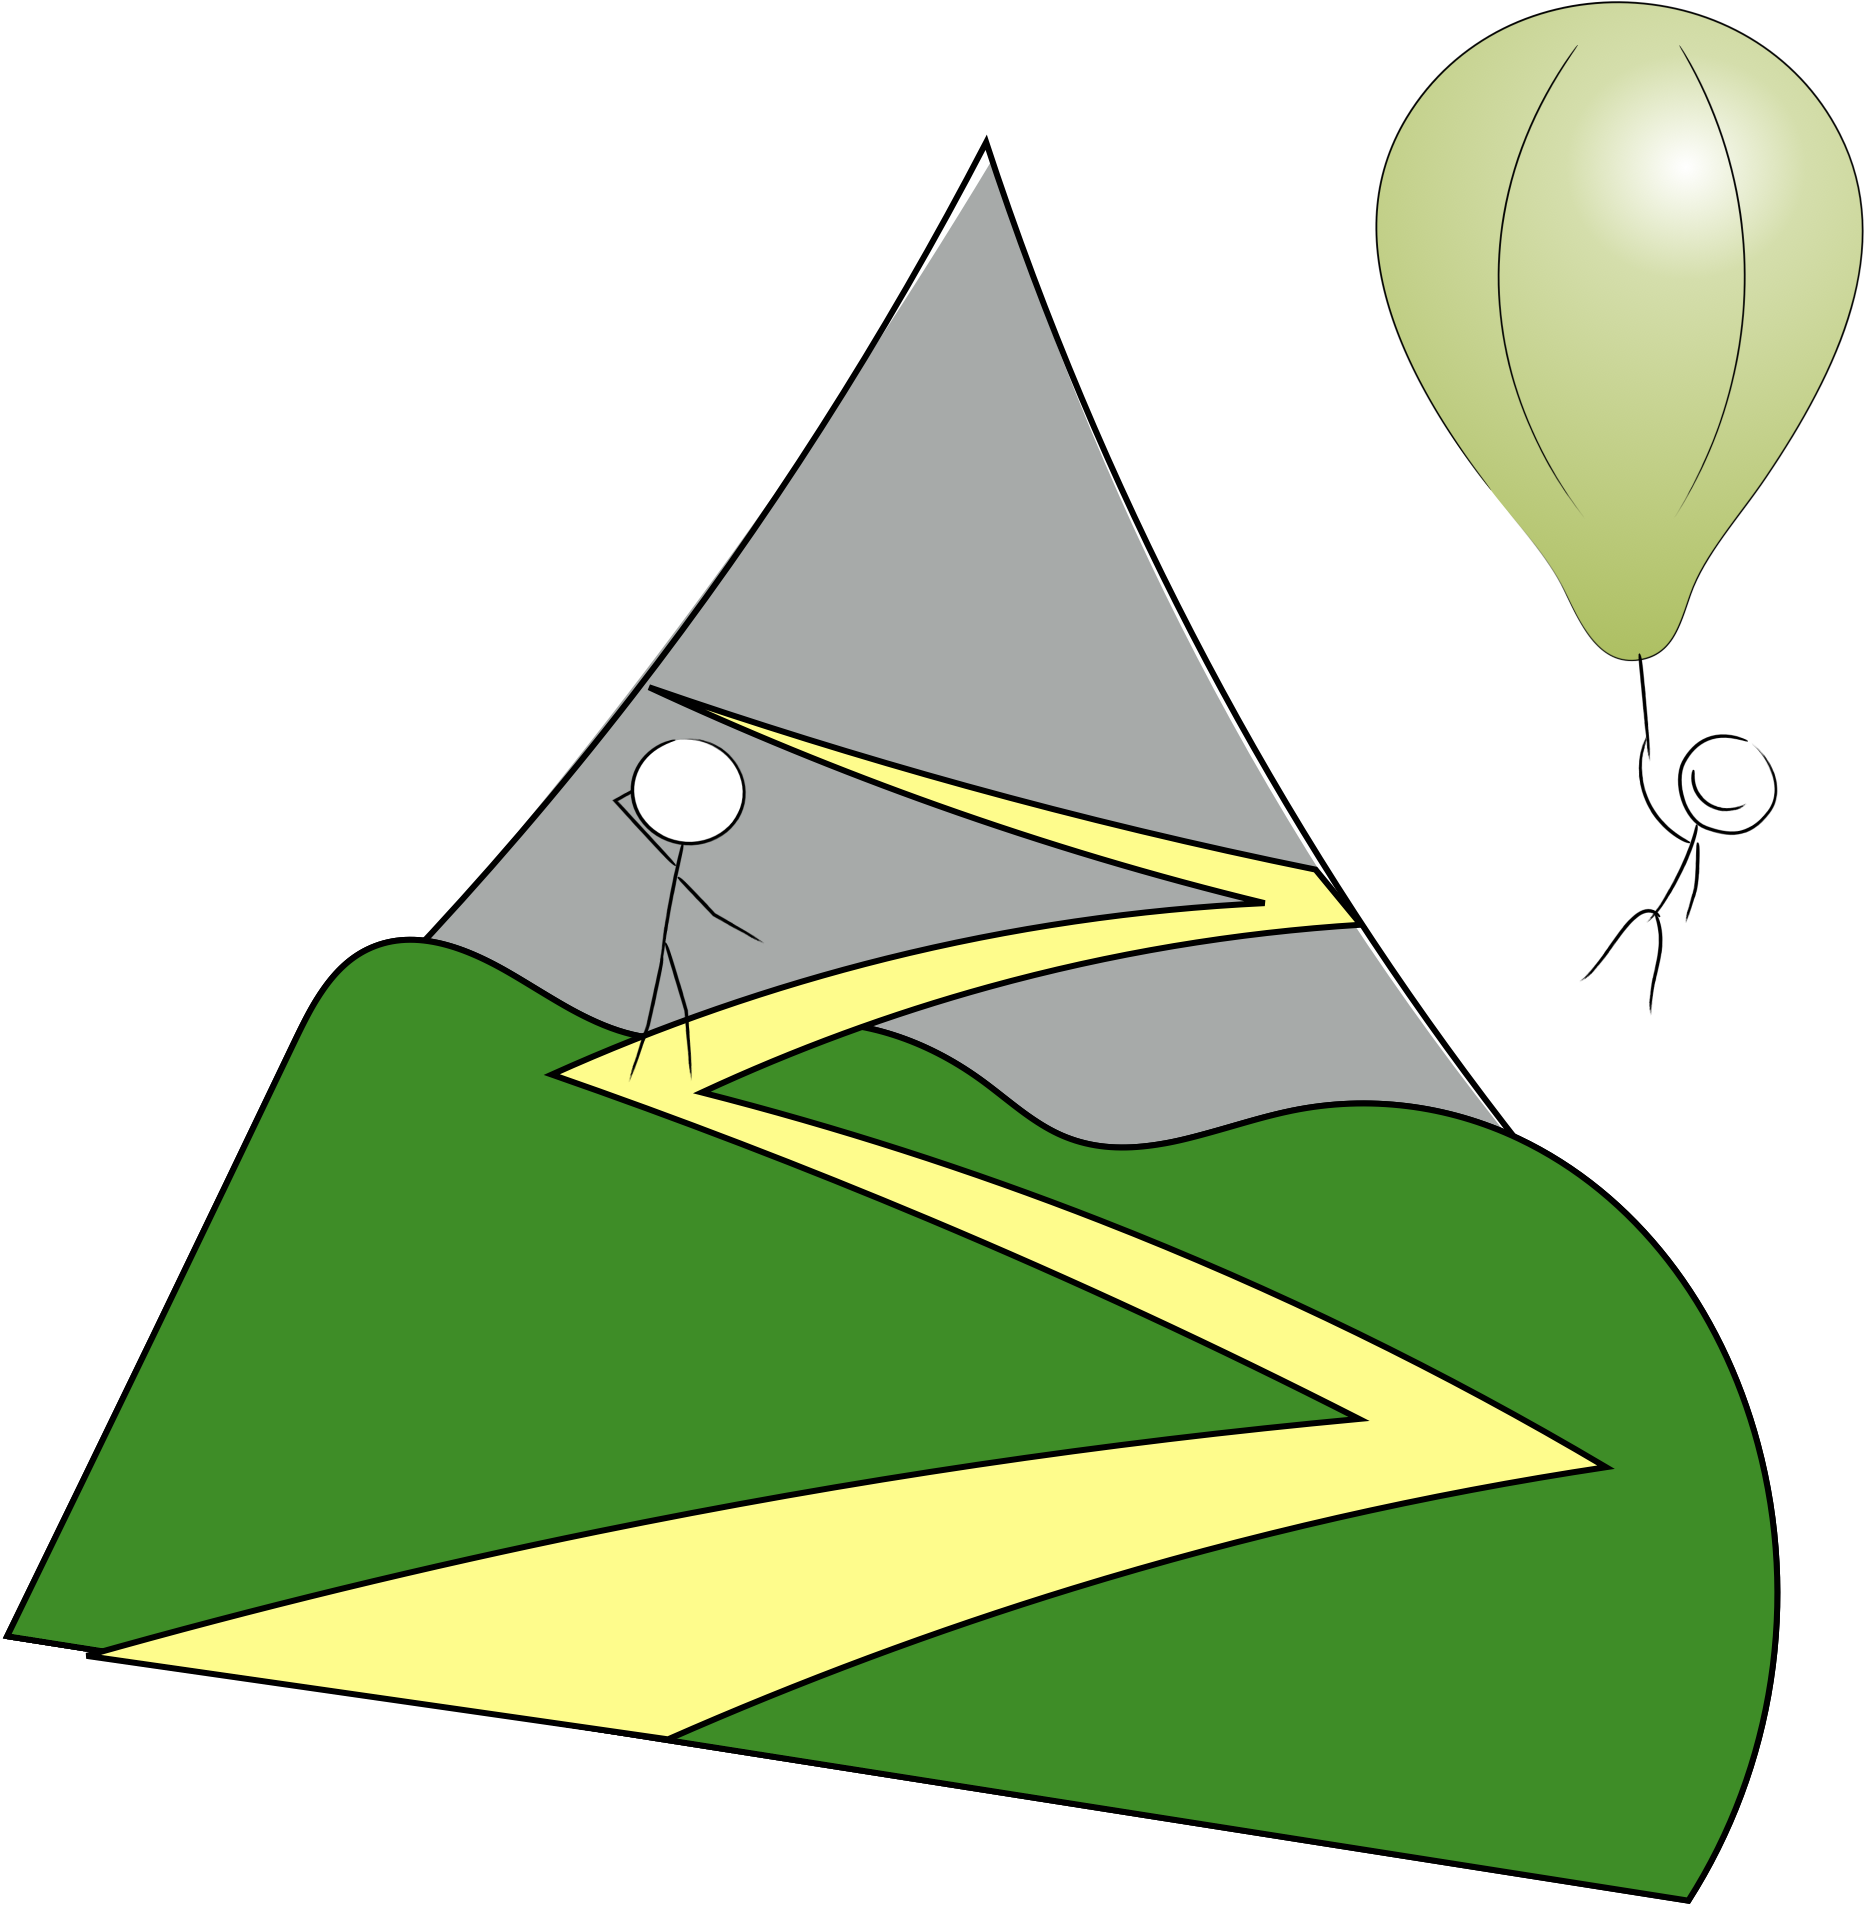
\includegraphics[width=0.3\linewidth]{images/mountain} 

}

\caption{State functions - no matter how you got here, here you are… …altitude is a good analogy for a state function, whether climbing the mountain or flying on the balloon if your altitude is 1000 m it is 1000 m!.}\label{fig:mountain}
\end{figure}

\hypertarget{sec:equations1}{%
\subsection{Useful equations - State functions}\label{sec:equations1}}

Hess' Law (Equation \eqref{eq:enthalpystate}) is something most will be familiar with already. You should try to think about it in terms of an equation however, not the cylces of which you may already be familiar.

\begin{equation}
\Delta_r H^{\ominus} = \sum_{products}v \Delta H^{\ominus}_\textrm{X}-\sum_{reactants}v \Delta H^{\ominus}_\textrm{X}
\label{eq:enthalpystate}
\end{equation}

Similar equations can be used for heat capacity (Equation \eqref{eq:heatcapacitystate}), this equation for heat capacity will then be used later in the course when we look at the effect of temperature on the enthalpy and entropy of reaction.

\begin{equation}
\Delta_r C_p^{\ominus} = \sum_{products}vC_{p,n}^{\ominus}-\sum_{reactants}vC_{p,n}^{\ominus}
\label{eq:heatcapacitystate}
\end{equation}

Entropy, just like enthalpy is a state function.

\begin{equation}
\Delta_r S^{\ominus} = \sum_{products}v S^{\ominus}-\sum_{reactants}v S^{\ominus}
\label{eq:entropystate}
\end{equation}

As is Gibbs' free energy.

\begin{equation}
\Delta _ r G^\ominus = \sum_{prod} v G_n^\ominus - \sum_{react} v  G_n^\ominus 
\label{eq:Gibbsstate}
\end{equation}

The value of each of these variables is independent of the path used to form them. Hence, the same \textbf{`products − reactants'} approach always works!

\hypertarget{sec:typesofsystem}{%
\section{Types of thermodynamic system}\label{sec:typesofsystem}}

When we consider anything in thermodynamics we have to consider both the system and its surroundings. The relationship between the system and the surroundings defines the different types of thermodynamic system.

\hypertarget{subsec:isolated}{%
\subsection{Isolated system}\label{subsec:isolated}}

\begin{figure}

{\centering 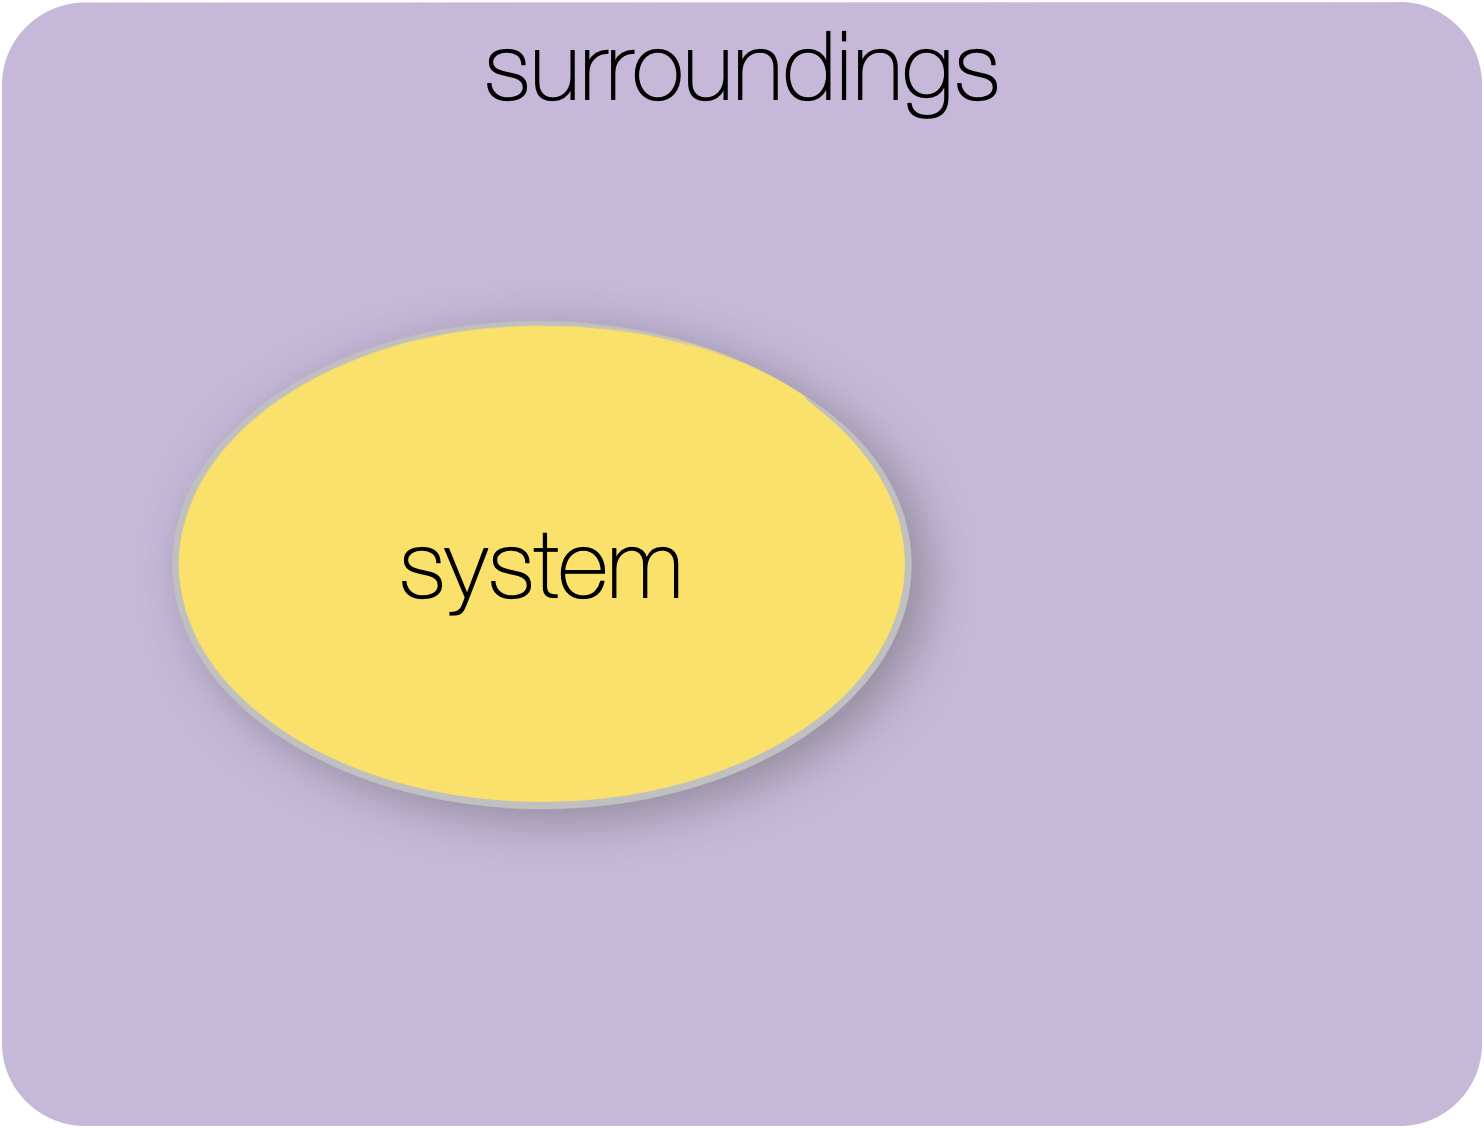
\includegraphics[width=0.3\linewidth]{images/isolated} 

}

\caption{Isolated system: there is no exchange of matter or energy between the system and surroundings.}\label{fig:isolated}
\end{figure}

In an isolated system, there can be no exchange of either matter or energy in any form between the system and surroundings.

A stoppered perfectly insulated flask may be thought of as an isolated system.

\hypertarget{subsec:open}{%
\subsection{Open system}\label{subsec:open}}

\begin{figure}

{\centering 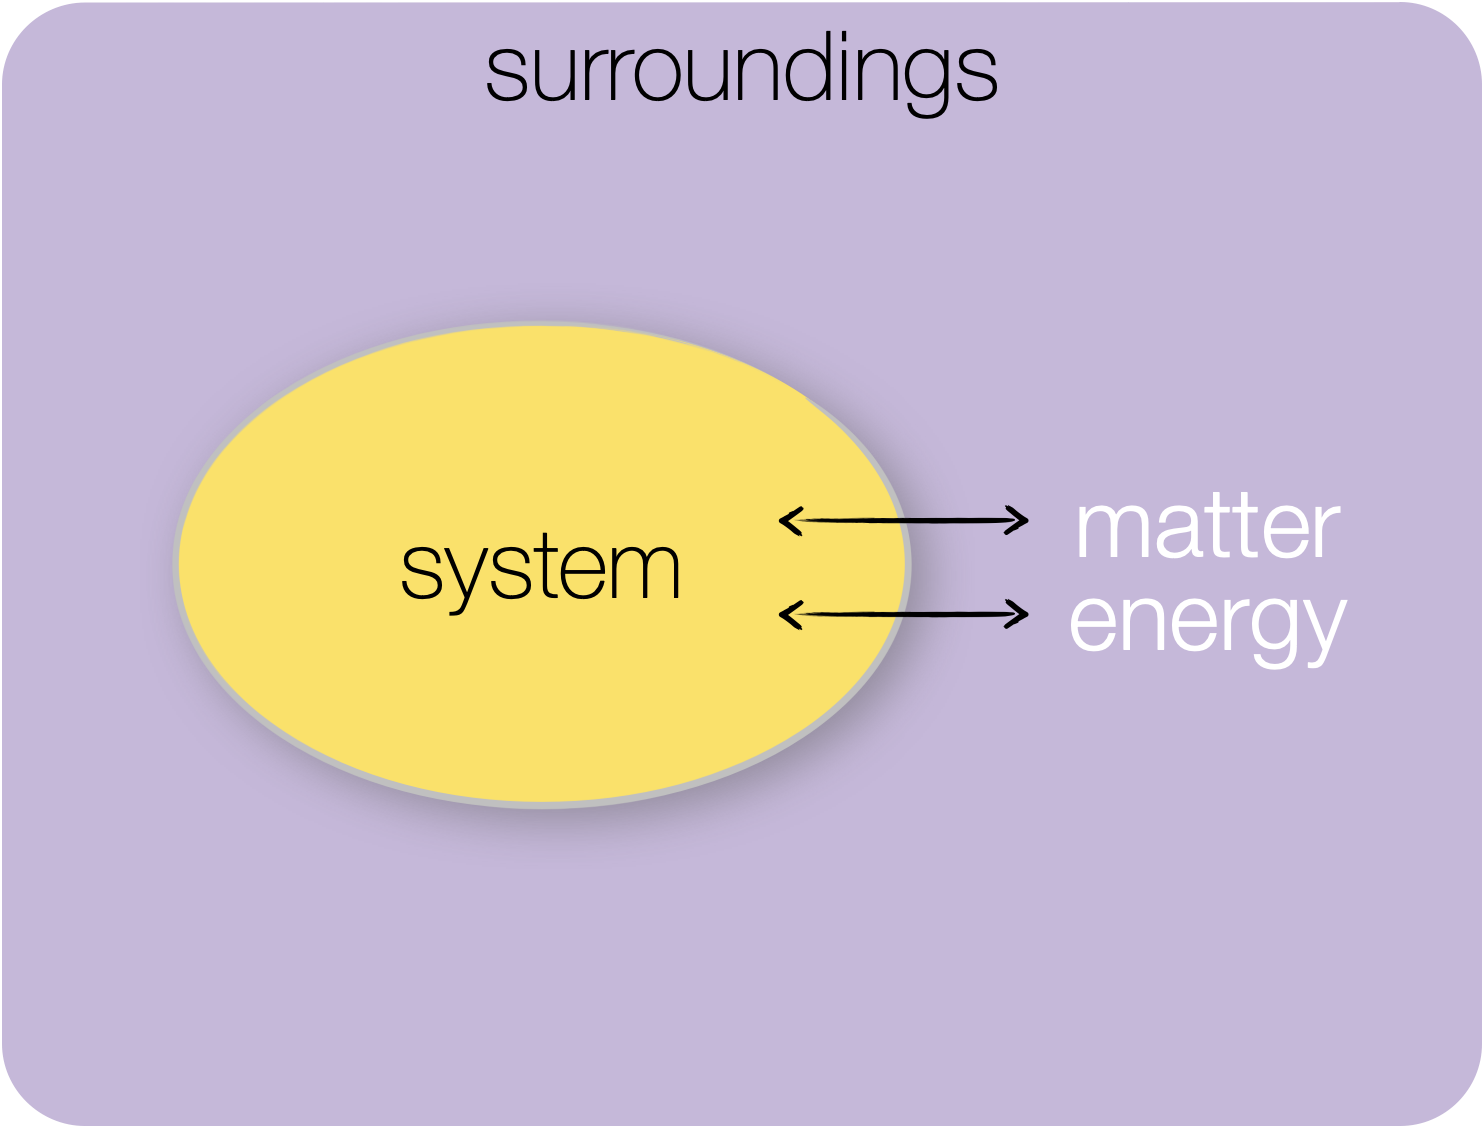
\includegraphics[width=0.3\linewidth]{images/open} 

}

\caption{Open system: in an open system both matter and energy may be exchanged between the system and surroundings.}\label{fig:open}
\end{figure}

In an open system both matter and energy can be exchanged between the system and surroundings.

A cup of tea is a nice example of an open system you can add sugar (if you are weird), drink it, or forget about it and find it cold 2 hours later.

\hypertarget{subsec:closed}{%
\subsection{Closed system}\label{subsec:closed}}

\begin{figure}

{\centering 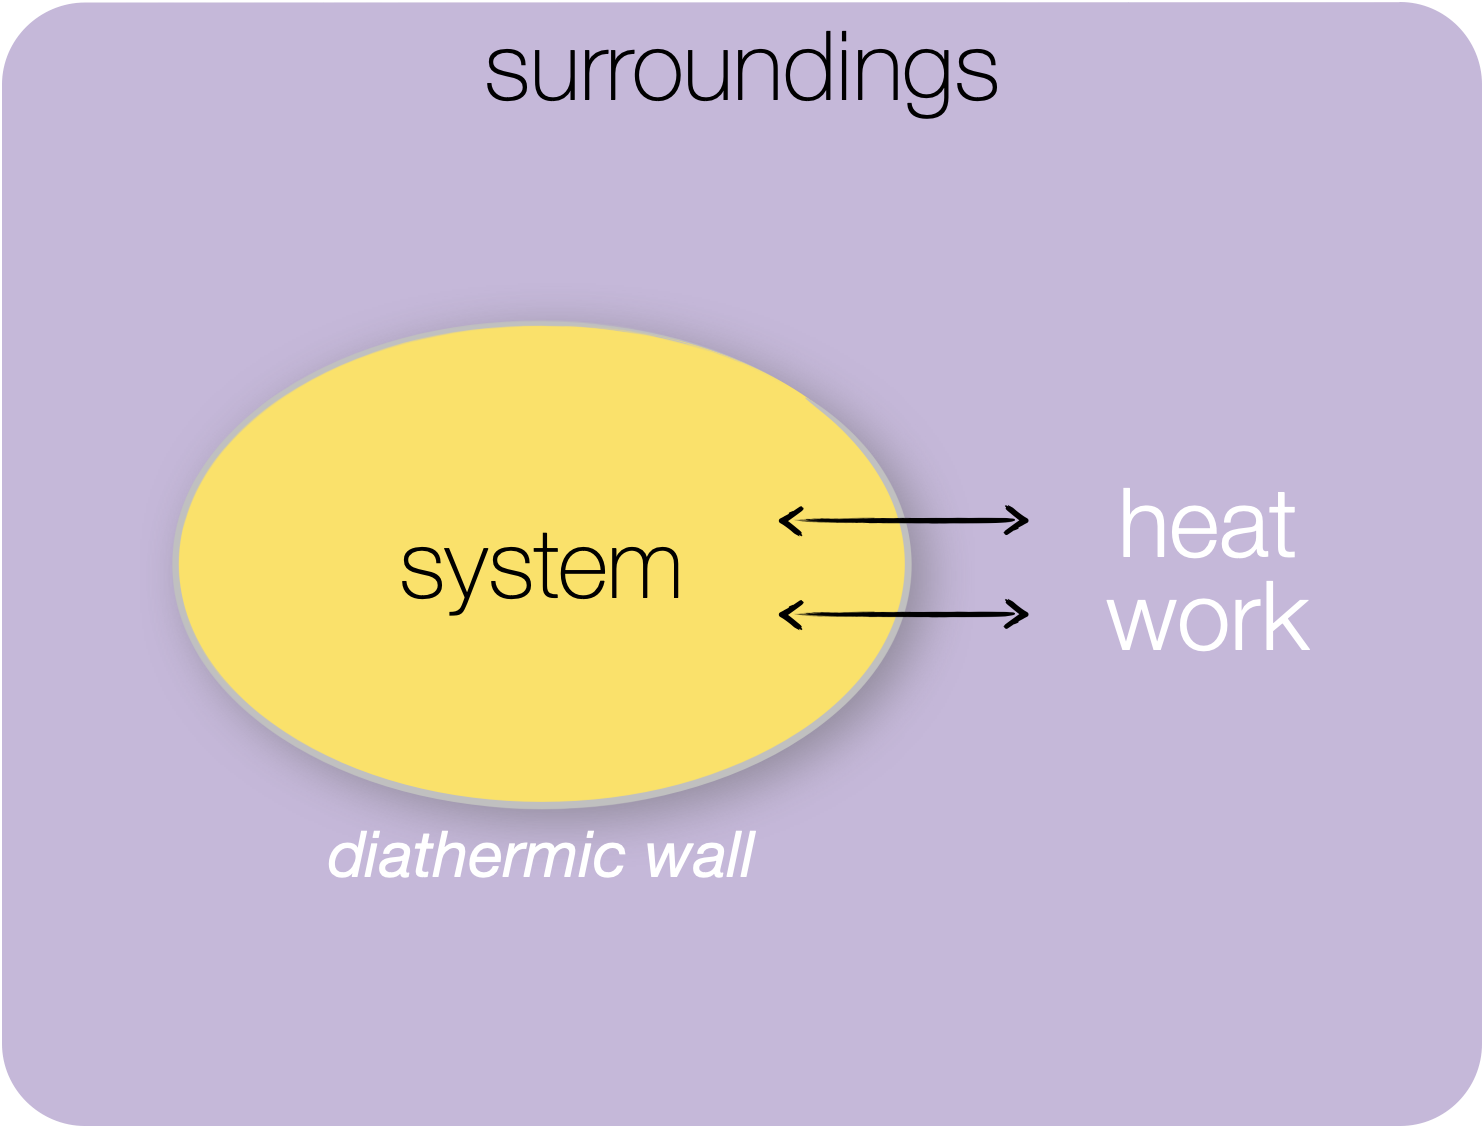
\includegraphics[width=0.3\linewidth]{images/closed} 

}

\caption{Closed system: in a closed system only energy in either the form of heat or work may be exchanged between system and surroundings..}\label{fig:closed}
\end{figure}

A closed system is one where you can't exchange matter but energy in the form of either `heat' or `work' can be exchanged between the system and surroundings.

A closed system is often used as a simpler model than an open system - not many things in life actually fit this model perfectly, but most bench chemistry where we can heat a system fits into this model.

\hypertarget{subsec:adiabatic}{%
\subsection{Adiabatic system}\label{subsec:adiabatic}}

\begin{figure}

{\centering 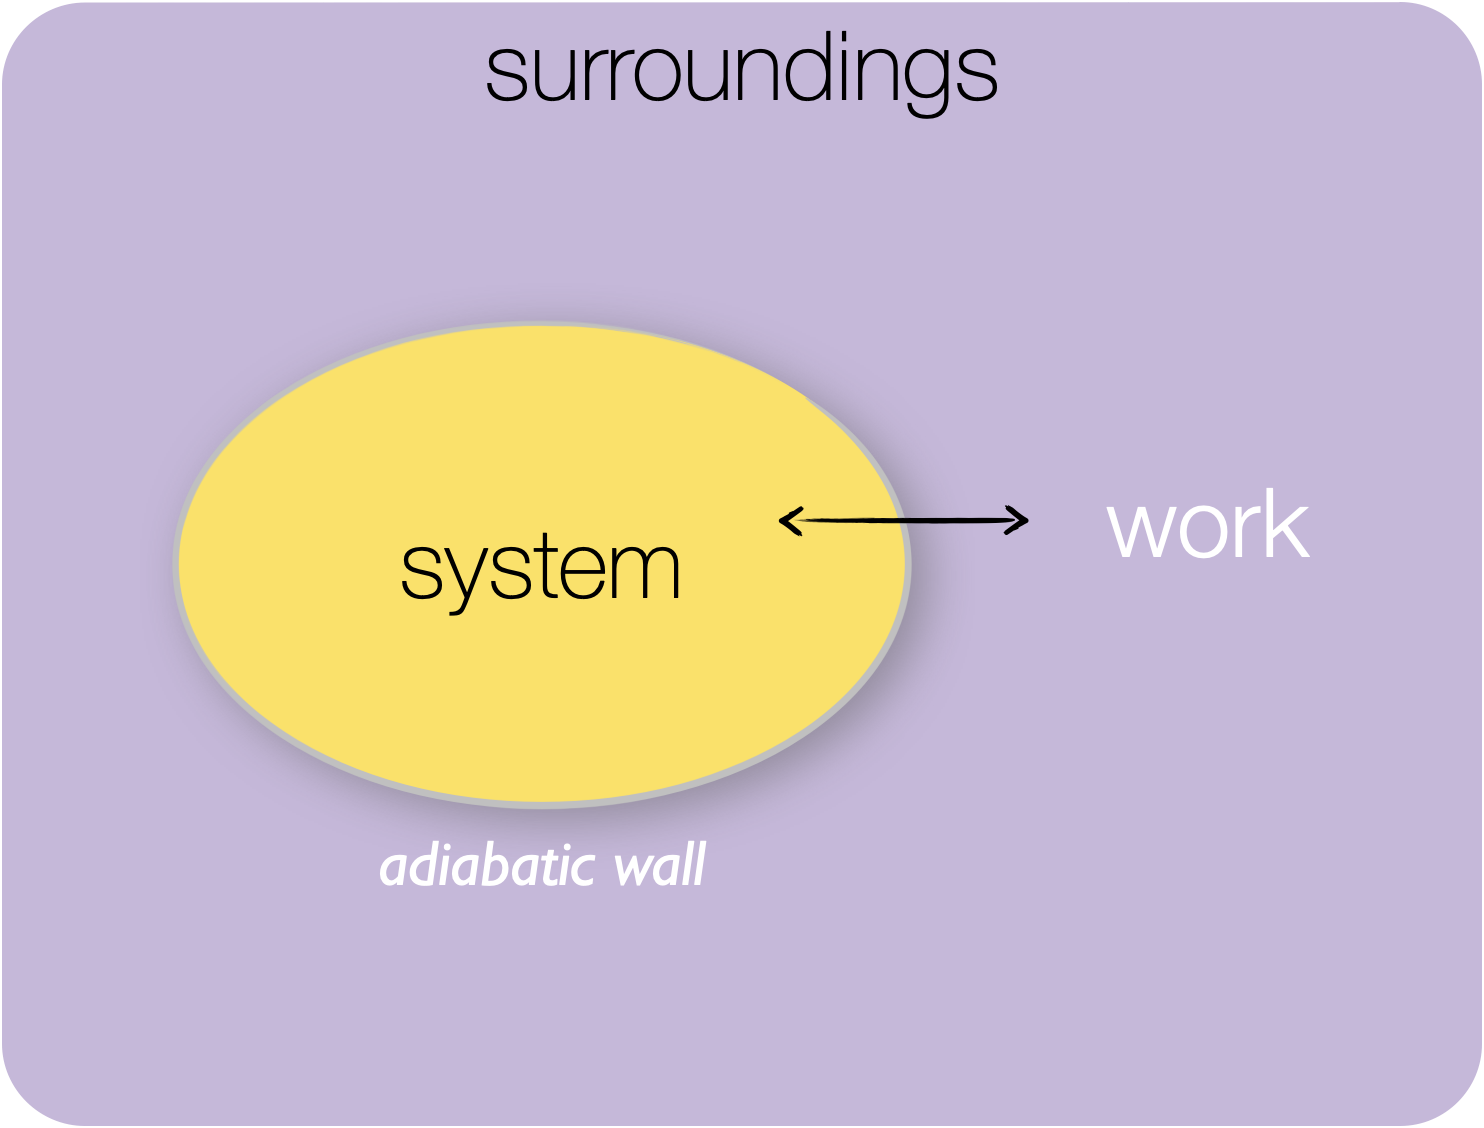
\includegraphics[width=0.3\linewidth]{images/adiabatic} 

}

\caption{Adiabatic system: in an adiabatic system only energy in the form of work may be exchanged between the system and surroundings.}\label{fig:adiabatic}
\end{figure}

An adiabatic system is one where you can't have any flow of heat between the system and surroundings, but you can exchange energy in the form of work.

This would mean that the system is insulated from the surroundings, and therefore the system may not be in thermodynamic equilibrium with the surroundings.

We will learn more about both `heat' and `work' later in the course.

\hypertarget{sec:extensiveintensive}{%
\section{Extensive and intensive properties}\label{sec:extensiveintensive}}

The difference between extensive and intensive properties is whether the property depends upon the amount of `stuff' you have.

\hypertarget{sec:intenstive}{%
\subsection{Intensive properties}\label{sec:intenstive}}

Properties which are \textbf{independent} of the amount of stuff are called \emph{`intensive properties'}.

Temperature is an example of an intensive property as are all of `molar' properties (the quantity of something `per mole'): molar heat capacity, molar enthalpy, molar entropy, molar Gibbs' energy, \emph{etc}\ldots{} in physics the term `specific' is often used such as specific heat capacity and specific enthalpy, these are also intensive properties based on the fixed amount of a `gram' (g).

\hypertarget{sec:extensive}{%
\subsection{Extensive properties}\label{sec:extensive}}

Conversely, properties which are \textbf{dependent} on the amount of stuff you have are called \emph{extensive properties}.

Many intensive properties have extensive equivalents, so whilst we have the intensive property `molar heat capacity' we also have extensive equivalent `heat capacity'; one looks at the amount of energy it takes to raise one mole of a thing by one kelvin, whereas the other looks at how much energy it takes to raise the temperature of how ever much of a thing we have by one kelvin.

Consequently extensive properties have different units to their `equivalent' intensive property.

Other examples of extensive properties are unsurprisingly: volume, mass, amount (as in moles), and length.

Whilst knowing the terms extensive and intensive isn't vital it is hugely important to recognise that sometimes terms will appear with different units to suit the particular situation.

\hypertarget{sec:classicalstat}{%
\section{\texorpdfstring{Classical \emph{vs.} Statistical thermodynamics}{Classical vs. Statistical thermodynamics}}\label{sec:classicalstat}}

Thermodynamics is quite an old subject, much of our understanding of why chemical reactions happen is based in 19th century science. This understanding was based on emperical observation of things like steam engines and battery piles. It scientists trying to understand how things work in order to make them better, make them more efficient, and make them safer.

This 19th century (and earlier) view of the world didn't even consider things we take for granted now, nowhere in thermodynamics do we ever really think about atoms. We talk about ideal systems (those that follow the rules nicely), but never really care about the reaction taking place, it is all just the bulk average behaviour of the system.

Then in the late 19th century Ludwig Boltzmann proposed a different way of thinking about thermodynamics. He started to think about the `average' behaviour of individual atoms. This version of statistical mechanics gave an explanation of what concepts like entropy were and it helped explain macroscopic phenomena (such as pressure and temperature) on an atomic and molecular level.

Statistical thermodynamics started to be able to explain the values of what had until then been emperical constants.

Consequently in this course we will look at thermodynamics from both a classical and statistical point of view.

\hypertarget{sec:degreesoffreedom}{%
\section{Degrees of Freedom}\label{sec:degreesoffreedom}}

Perhaps unsurprisingly the structure of molecules is an important concept when we consider thermodynamics from the molecule up perspective, but perhaps surprisingly classical thermodynamics does not care at all the structure of the molecules in the system we are considering.

\begin{figure}

{\centering 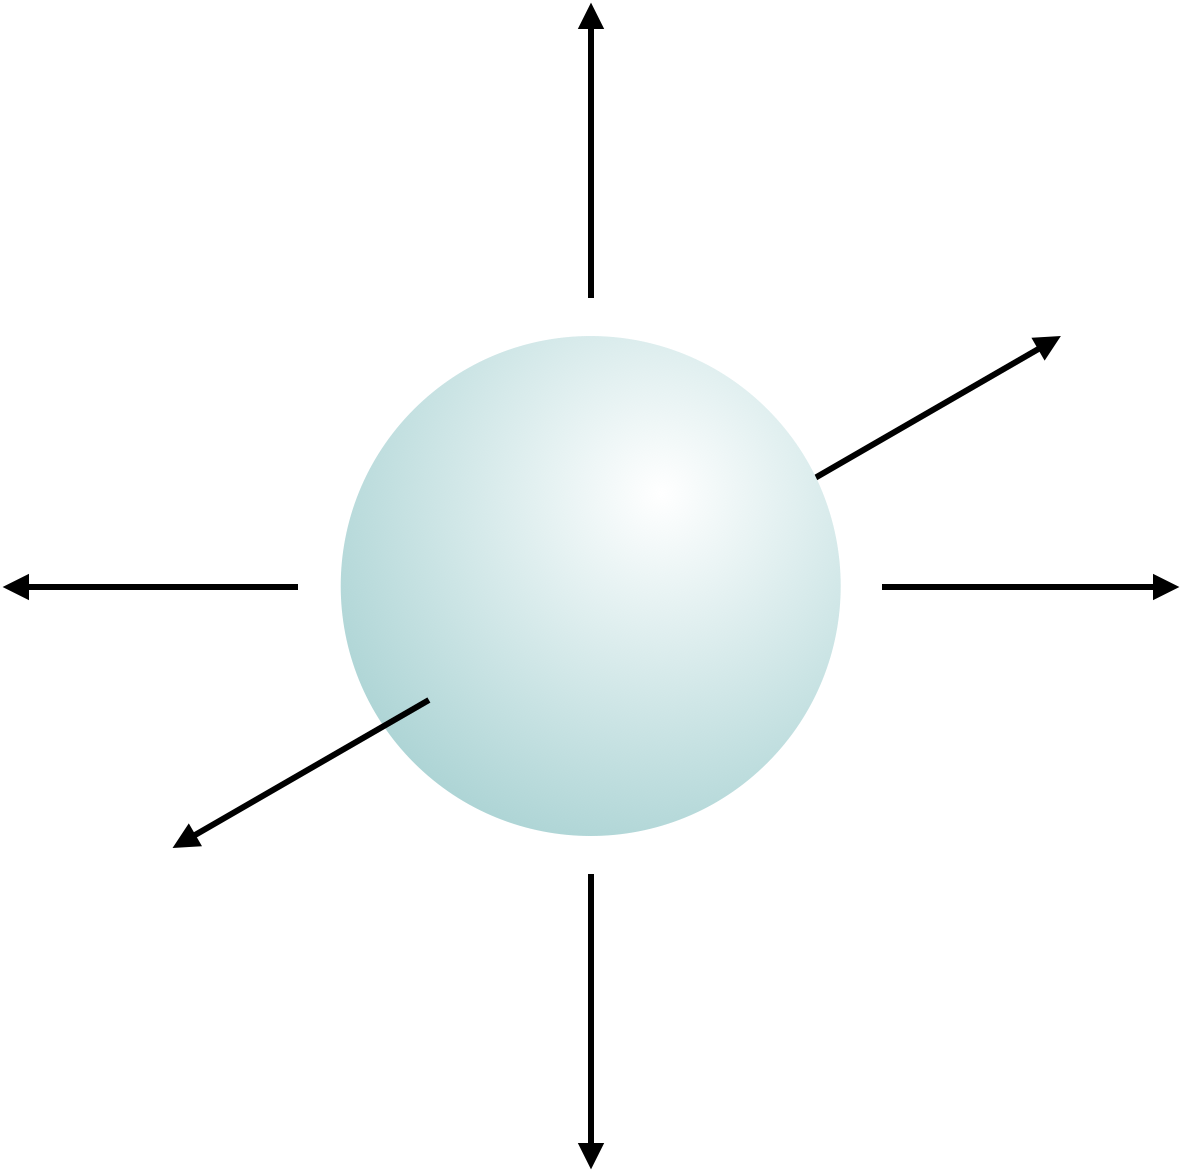
\includegraphics[width=0.3\linewidth]{images/atomdegrees} 

}

\caption{Every atom has three degrees of freedom, these are movement along the x, y and z axis.}\label{fig:atomdegrees}
\end{figure}

When atoms combine to form moleucules the total number of degrees of freedom must be conserved, and so new types of degrees of freedom are introduced, namely molecular rotations and molecular vibrations (figure \ref{fig:typesdegree}, and equations \eqref{eq:lineardof} and \eqref{eq:nonlineardof}).

\begin{figure}

{\centering 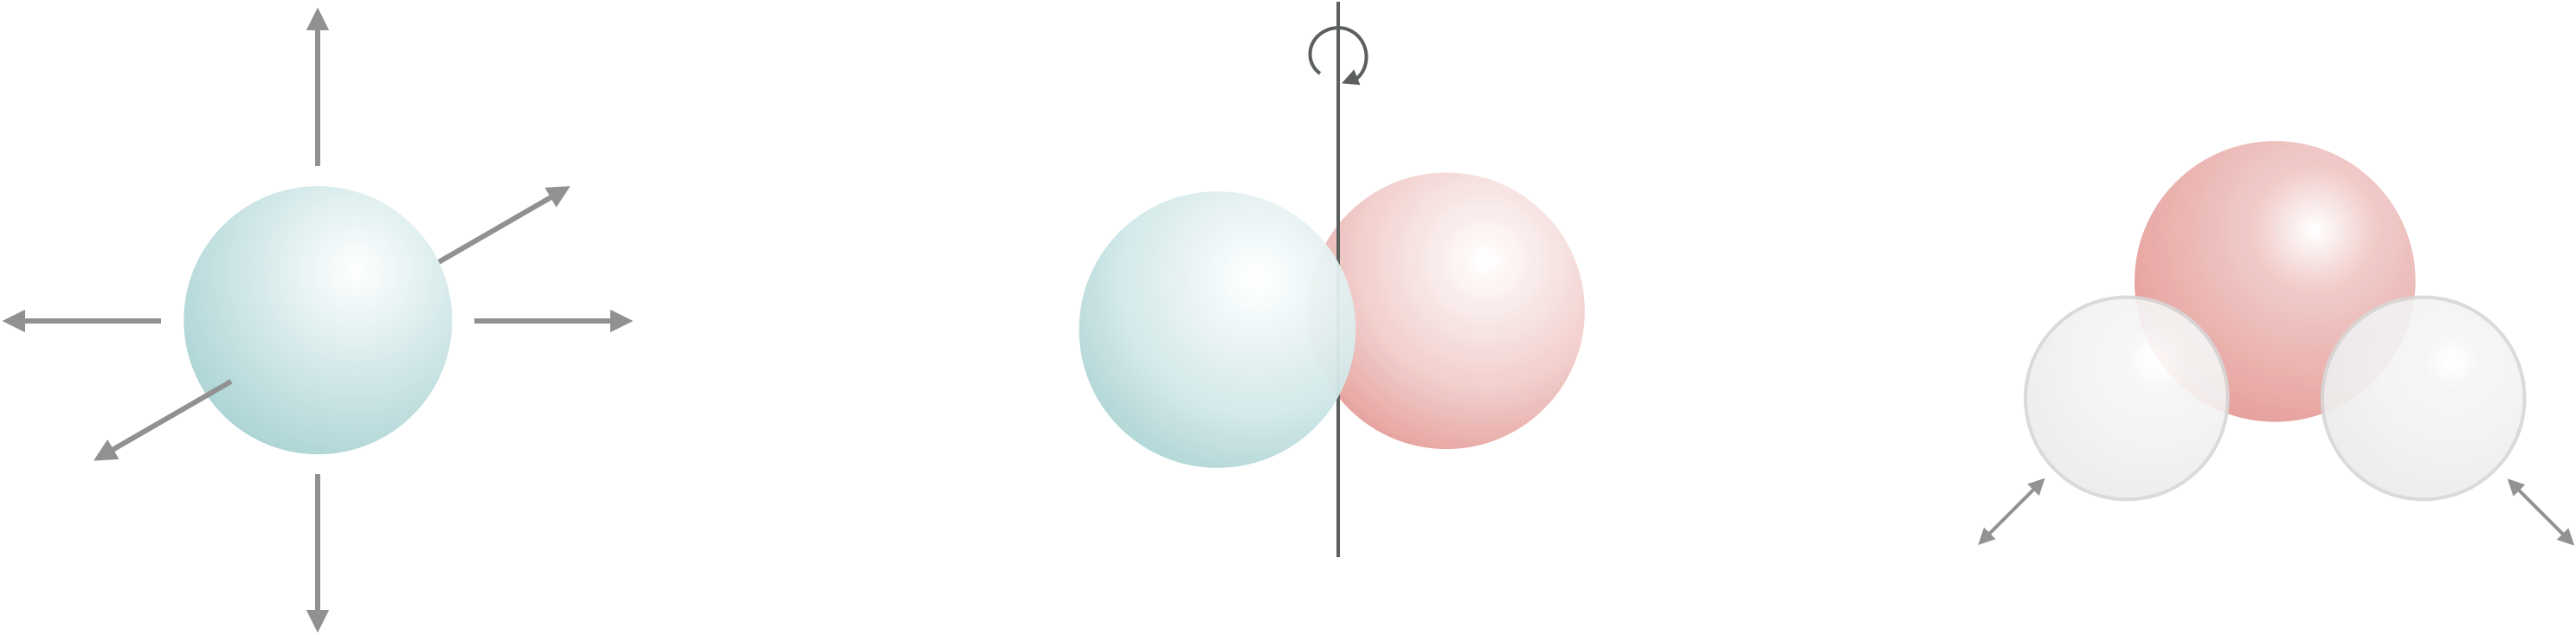
\includegraphics[width=0.8\linewidth]{images/typesdegree} 

}

\caption{Translations, molecular rotations and molecular vibrations are all degrees of freedom.}\label{fig:typesdegree}
\end{figure}

For linear molecules there are three translational degrees of freedom, two rotational degrees of freedom (figure \ref{fig:linear}) and the number of vibrational degrees of freedom is given by equation \eqref{eq:lineardof}, where N is the total number of atoms in the molecule:

\begin{equation}
x = 3N-5
\label{eq:lineardof}
\end{equation}

\begin{figure}

{\centering 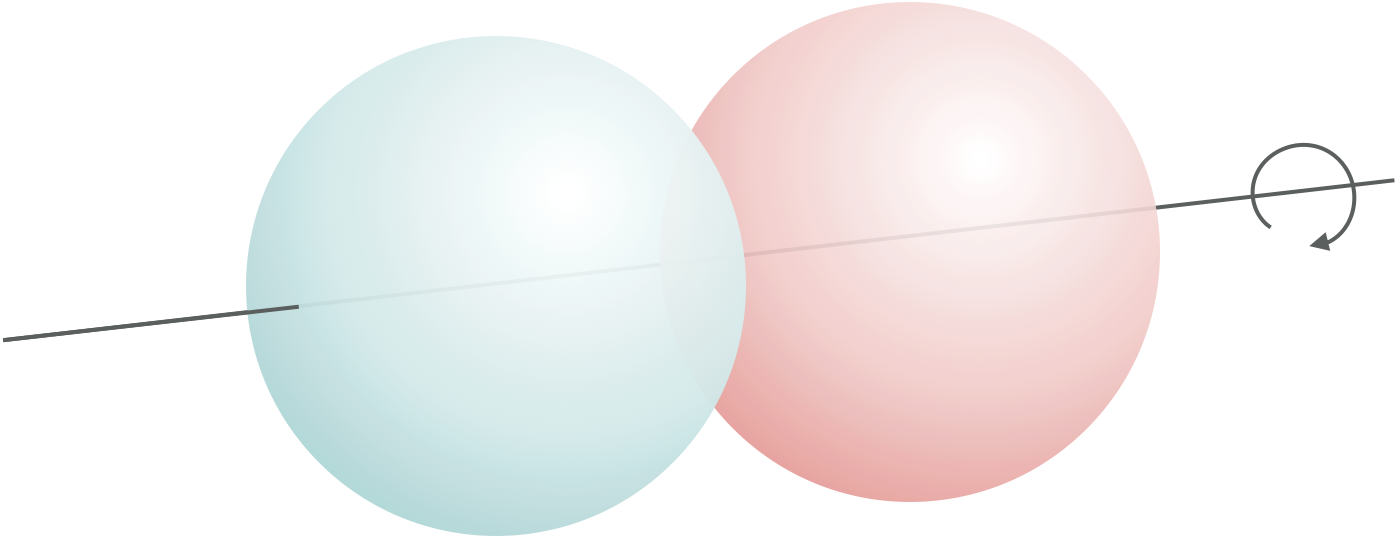
\includegraphics[width=0.5\linewidth]{images/linear} 

}

\caption{In linear molecules there are only two rotational degrees of freedom as rotaion around the z-axis (the long axis of the molecule) are equivalent and therefore dont contribute to the degrees of freedom.}\label{fig:linear}
\end{figure}

For non-linear molecules there are three translational degrees of freedom, three rotational degrees of freedom and the number of vibrational degrees of freedom is given by equation \eqref{eq:nonlineardof}, again where N is the total number of atoms in the molecule:

\begin{equation}
x = 3N-6
\label{eq:nonlineardof}
\end{equation}

\hypertarget{example-calculations}{%
\section{Example calculations}\label{example-calculations}}

\hypertarget{sec:examplehess}{%
\subsection{Example calculation - Hess's Law}\label{sec:examplehess}}

How much energy is released when 4.60 g of sodium reacts with excess water to give NaOH (aq) \& H\textsubscript{2} (g)?

\begin{itemize}
\tightlist
\item
  ΔH\textsubscript{f}\textsuperscript{⦵} NaOH = −425.61 kJ mol\textsuperscript{−1}
\item
  ΔH\textsubscript{f}\textsuperscript{⦵} H\textsubscript{2}O = −285.83 kJ mol\textsuperscript{−1}
\end{itemize}

The enthalpy of formation of elements in their standard state (\emph{e.g.} Na (s) \& H\textsubscript{2} (g)) is zero.

Therefore using equation \eqref{eq:enthalpystate}:

\begin{equation*}
\Delta H_{rxn}^{\ominus}= \Delta H_{f}^{\ominus}(\textrm{NaOH})-\Delta H_{f}^{\ominus}(\textrm{H}_2\textrm{O})= −425.61 \textrm{ kJ mol}^{−1} − −285.83 \textrm{ kJ mol}^{−1} = −139.78 \textrm{ kJ mol}^{−1}
\end{equation*}

\(R_M \textrm{ Na} = 22.989769 \textrm{ g mol}^{−1}\)
Therefore:

\begin{equation*}
n \textrm{(Na)} = \frac{m}{R_M} = \frac{4.60 \textrm{ g}}{ 22.989769 \textrm{ g mol}^{−1}} = 0.200 \textrm{ mol}
\end{equation*}

\emph{note sf!}

Therefore if 4.60g reacts:

\begin{equation*}
\Delta H_{rxn}^⦵ ( \textrm{kJ}) = \Delta H_{rxn}^⦵ ( \textrm{kJ mol}^{−1}) × \textrm{mol} = −139.78 \textrm{kJ mol}^{-1} × 0.200 \textrm{mol} = −28.0 \textrm{ kJ}
\end{equation*}

The `−' sign indicates that heat is released (evolved) and the temperature of the surroundings increases.

\hypertarget{subsec:examplekirchoff}{%
\subsection{Example Calculation - Kirchoff's law}\label{subsec:examplekirchoff}}

Kirchoff's laws may be used to adjust calculated values of enthalpy and entropy of reaction to different temperatures, they use the difference in heat capacity of products and reactants to do this. Determine \(ΔC_{p,m}\) for the following reaction:

CH\textsubscript{3}CH\textsubscript{2}OH (aq) + CH\textsubscript{3}COOH (aq) ⟶ CH\textsubscript{3}COOCH\textsubscript{2}CH\textsubscript{3} (aq) + H\textsubscript{2}O (l)

\begin{longtable}[]{@{}cc@{}}
\toprule
& \(ΔC_{p,m}\) / J K\(^{−1}\) mol\(^{−1}\)\tabularnewline
\midrule
\endhead
CH\textsubscript{3}CH\textsubscript{2}OH (aq) & 111.46\tabularnewline
CH\textsubscript{3}COOH (aq) & 124.3\tabularnewline
CH\textsubscript{3}COOCH\textsubscript{2}CH\textsubscript{3} (aq) & 170.1\tabularnewline
H\textsubscript{2}O (l) & 33.58\tabularnewline
\bottomrule
\end{longtable}

\begin{equation*}
ΔC_{p,m \textrm{ rxn}} = (C_{p,m} \textrm{CH$_3$COOCH$_2$CH$_3$ (aq)} + C_{p,m} \textrm{H$_2$O (l)}) − (C_{p,m} \textrm{CH$_3$CH$_2$OH (aq)} + C_{p,m} \textrm{CH$_3$COOH (aq)})
\end{equation*}

\begin{equation*}
ΔC_\textrm{p,m rxn} = (170.1 + 33.58) − (111.46 + 124.3) \textrm{ J K$^{-1}$ mol}^{−1}) = − 32.1 \textrm{ J K$^{-1}$ mol}^{−1}
\end{equation*}

\hypertarget{subsec:exampledegreesoffreedom}{%
\subsection{Example Calculation - Degrees of Freedom}\label{subsec:exampledegreesoffreedom}}

Determine the number of degrees of freedom, and types of each, of ethanol CH\textsubscript{3}CH\textsubscript{2}OH.

Ethanol is non-linear molecule with 9 atoms. Therefore in total there are (3N) 27 degrees of freedom.

There will be 3 translational degrees of freedom (along the x,y\&z axes),

there will be 3 rotational degrees of freedom (rotation around the x,y\&z axes),

and there will be 3N-6 (because it is non linear) or 21 vibrational degrees of freedom.

\hypertarget{sec:Questions1}{%
\section{Questions}\label{sec:Questions1}}

Later in this course you will learn about the origin of these equations, for now it is enough to be able to balance chemical equations and use the fact that each of the variables in the following equations are state functions.

\begin{enumerate}
\def\labelenumi{\arabic{enumi}.}
\tightlist
\item
  What is the standard Gibbs' free energy of the oxidation of ammonia (NH\textsubscript{3}) to nitric acid (NO)?
\end{enumerate}

Hint: This is a redox reaction.

\(ΔG^⦵_{f, \textrm{NH}_3} = −16.45 \textrm{ kJ mol}^{−1}\)

\(ΔG^⦵_{f, \textrm{NO}} = +86.55 \textrm{ kJ mol}^{−1}\)

\(ΔG^⦵_{f, \textrm{H}_2 \textrm{O}} = −228.57 \textrm{ kJ mol}^{−1}\)

\begin{center}\rule{0.5\linewidth}{0.5pt}\end{center}

\begin{enumerate}
\def\labelenumi{\arabic{enumi}.}
\setcounter{enumi}{1}
\tightlist
\item
  Methanol fuel cells have been proposed as replacements for internal combustion engines. Methanol (density, ρ = 792 kg m\textsuperscript{−3}) is reacted in a fuel cell to be completely oxidised.
\end{enumerate}

Given the enthalpies of formation required are listed below determine the amount of energy released per mL of methanol.

\(ΔH^⦵_{f, \textrm{CH}_3\textrm{OH}} = −425.61 \textrm{ kJ mol}^{−1}\)

\(ΔH^⦵_{f, \textrm{H}_2 \textrm{O}} = −241.82 \textrm{ kJ mol}^{−1}\)

\(ΔH^⦵_{f, \textrm{CO}_2} = −393.51 \textrm{ kJ mol}^{−1}\)

\begin{center}\rule{0.5\linewidth}{0.5pt}\end{center}

\begin{enumerate}
\def\labelenumi{\arabic{enumi}.}
\setcounter{enumi}{2}
\tightlist
\item
  Ammonium dichromate decomposes upon heating in a spectacular `volcano' reaction:
\end{enumerate}

(NH\textsubscript{4})\textsubscript{2}Cr\textsubscript{2}O\textsubscript{7} (s) ⟶ N\textsubscript{2} (g) + 4 H\textsubscript{2}O (g) + Cr\textsubscript{2}O\textsubscript{3} (s)

Determine the enthalpy of reaction for this process given the following data.

\(ΔH^⦵_{f, \textrm{(NH}_4\textrm{)Cr}_2\textrm{O}_7\textrm{ (s)}} = −1810 \textrm{ kJ mol}^{−1}\)

\(ΔH^⦵_{f, \textrm{H}_2 \textrm{O (g)}} = −240 \textrm{ kJ mol}^{−1}\)

\(ΔH^⦵_{f, \textrm{Cr}_2 \textrm{O}_3 \textrm{ (g)}} = −1140 \textrm{ kJ mol}^{−1}\)

How would the enthalpy of reaction differ if liquid water was formed? Justify your answer.

\hypertarget{sec:Answers1}{%
\section{Answers}\label{sec:Answers1}}

\begin{enumerate}
\def\labelenumi{\arabic{enumi}.}
\tightlist
\item
  \(ΔG_{rxn}^⦵\) = −239.86 kJ mol\textsuperscript{−1}\(_{NH_3}\) (per mole of NH\textsubscript{3})
\item
  \(ΔH_{rxn}^⦵\) = -11.2 kJ cm\textsuperscript{-3}
\item
  \(ΔH_{rxn}^⦵\) = -290 kJ mol\textsuperscript{−1}, become more negative as heat is released upon condensing (we will cover this later in the course if you don't understant this last part, please don't stress).
\end{enumerate}

\hypertarget{ch:Part2}{%
\chapter{Week 1 - Part 2}\label{ch:Part2}}

There are different methods of teaching thermodynamics, many come at the problem from a very mathematical viewpoint, with partial derivatives, and operators. This course does not do that, the emphasis here is on understanding thermodynamic concepts, and being able to apply them solve problems. At no point will I expect you to be able to derive something, and I only include the derivations of a couple of equations where I feel it aids understanding of the concept.

If you wish to see a more mathematical version of this course it is covered in a number of textbooks, including the recommended text for this course, Atkin's Elements of Physical Chemistry.

\hypertarget{sec:zeroth}{%
\section{Zeroth Law of Thermodynamics}\label{sec:zeroth}}

There are four laws of thermodynamics, each introduces a thermodynamic concept. The first of these laws was actually the last to be defined and is called the \emph{zeroth law}.

The zeroth law deals with the idea of thermal equilibrium, and leads to the concept of \emph{temperature}.

\begin{figure}

{\centering 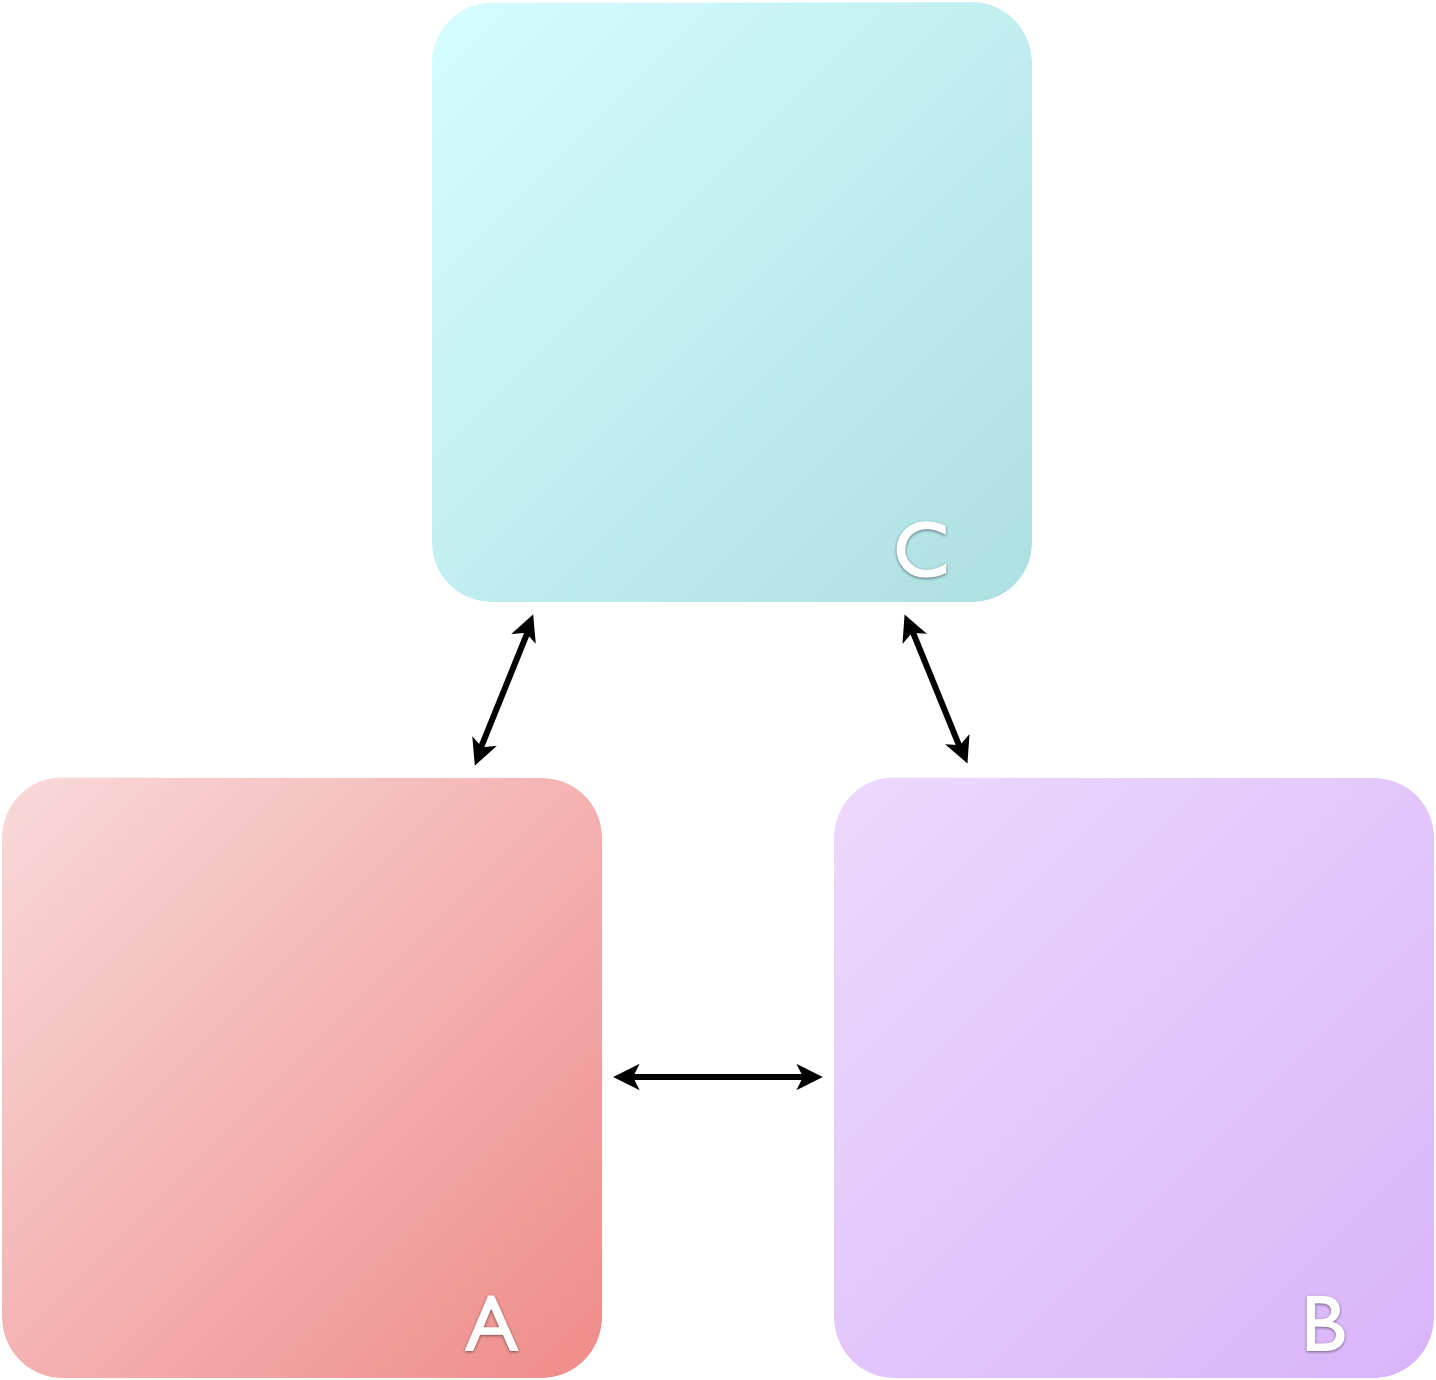
\includegraphics[width=0.5\linewidth]{images/thermalequilibrium} 

}

\caption{The zeroth law of thermodynamics states: if A is in thermal equilibrium with B, and B is in thermal equilibrium with C, then C will be in thermal equilibrium with A.}\label{fig:zerothlaw}
\end{figure}

The thermal equilibrium used in figure \ref{fig:zerothlaw} basically says that if A and B are in thermal equilibrium then they must have the same temperature. Therefore the first thermodynamic concept we meet is temperature, which has the unit K (kelvin).

\emph{The following video is for context and interest only}

\hypertarget{what-is-temperature}{%
\section{What is temperature?}\label{what-is-temperature}}

You are already familiar with the Maxwell-Boltzmann distribution, and have seen that the mean speed of a gas particle depends only upon the mass of that particle and the temperature (figure \ref{fig:boltzmann}).

\begin{figure}

{\centering 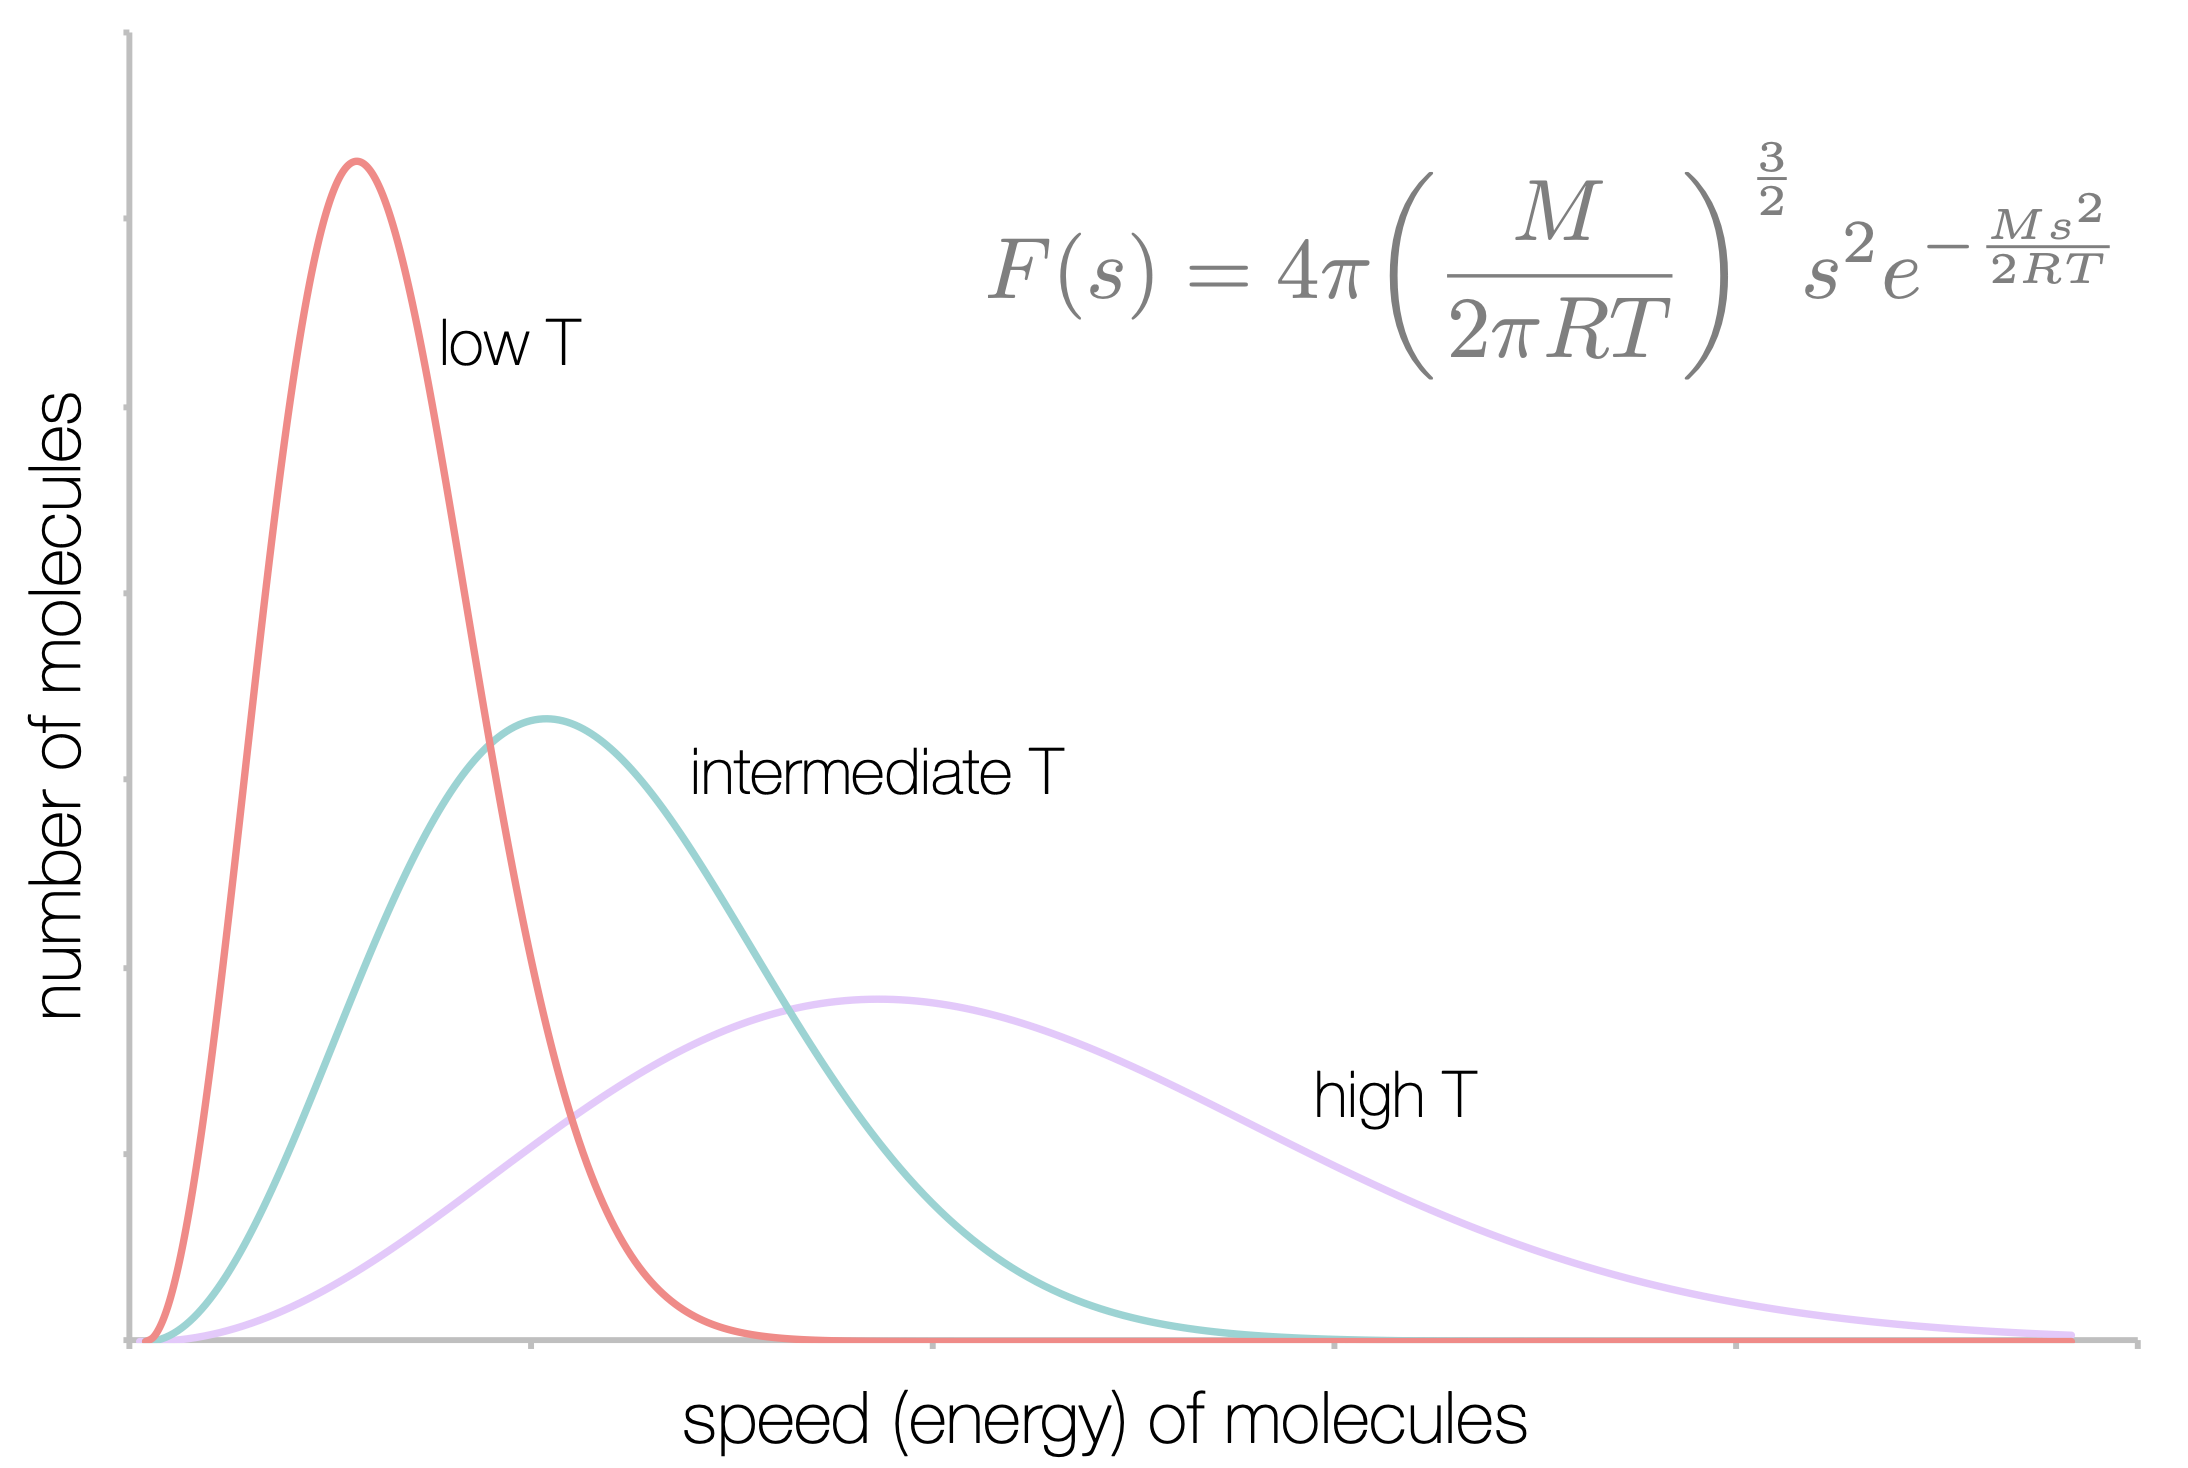
\includegraphics[width=0.8\linewidth]{images/boltzmann} 

}

\caption{The distribution of speeds of a gas depends only upon temperature and molecular mass. At low temperatures the mean speeds of particles are lower than those at high temperatures.}\label{fig:boltzmann}
\end{figure}

Therefore there is fundamental link between `speed' and temperature. In Section \ref{sec:classicalstat} you were introduced to the concept of energy levels in molecules. If you recall all energy levels are quantised, and translational energy levels have the closest spacing (figure \ref{fig:energylevels}). The faster a molecule moves the higher the translational energy level it occupies.

\begin{figure}

{\centering 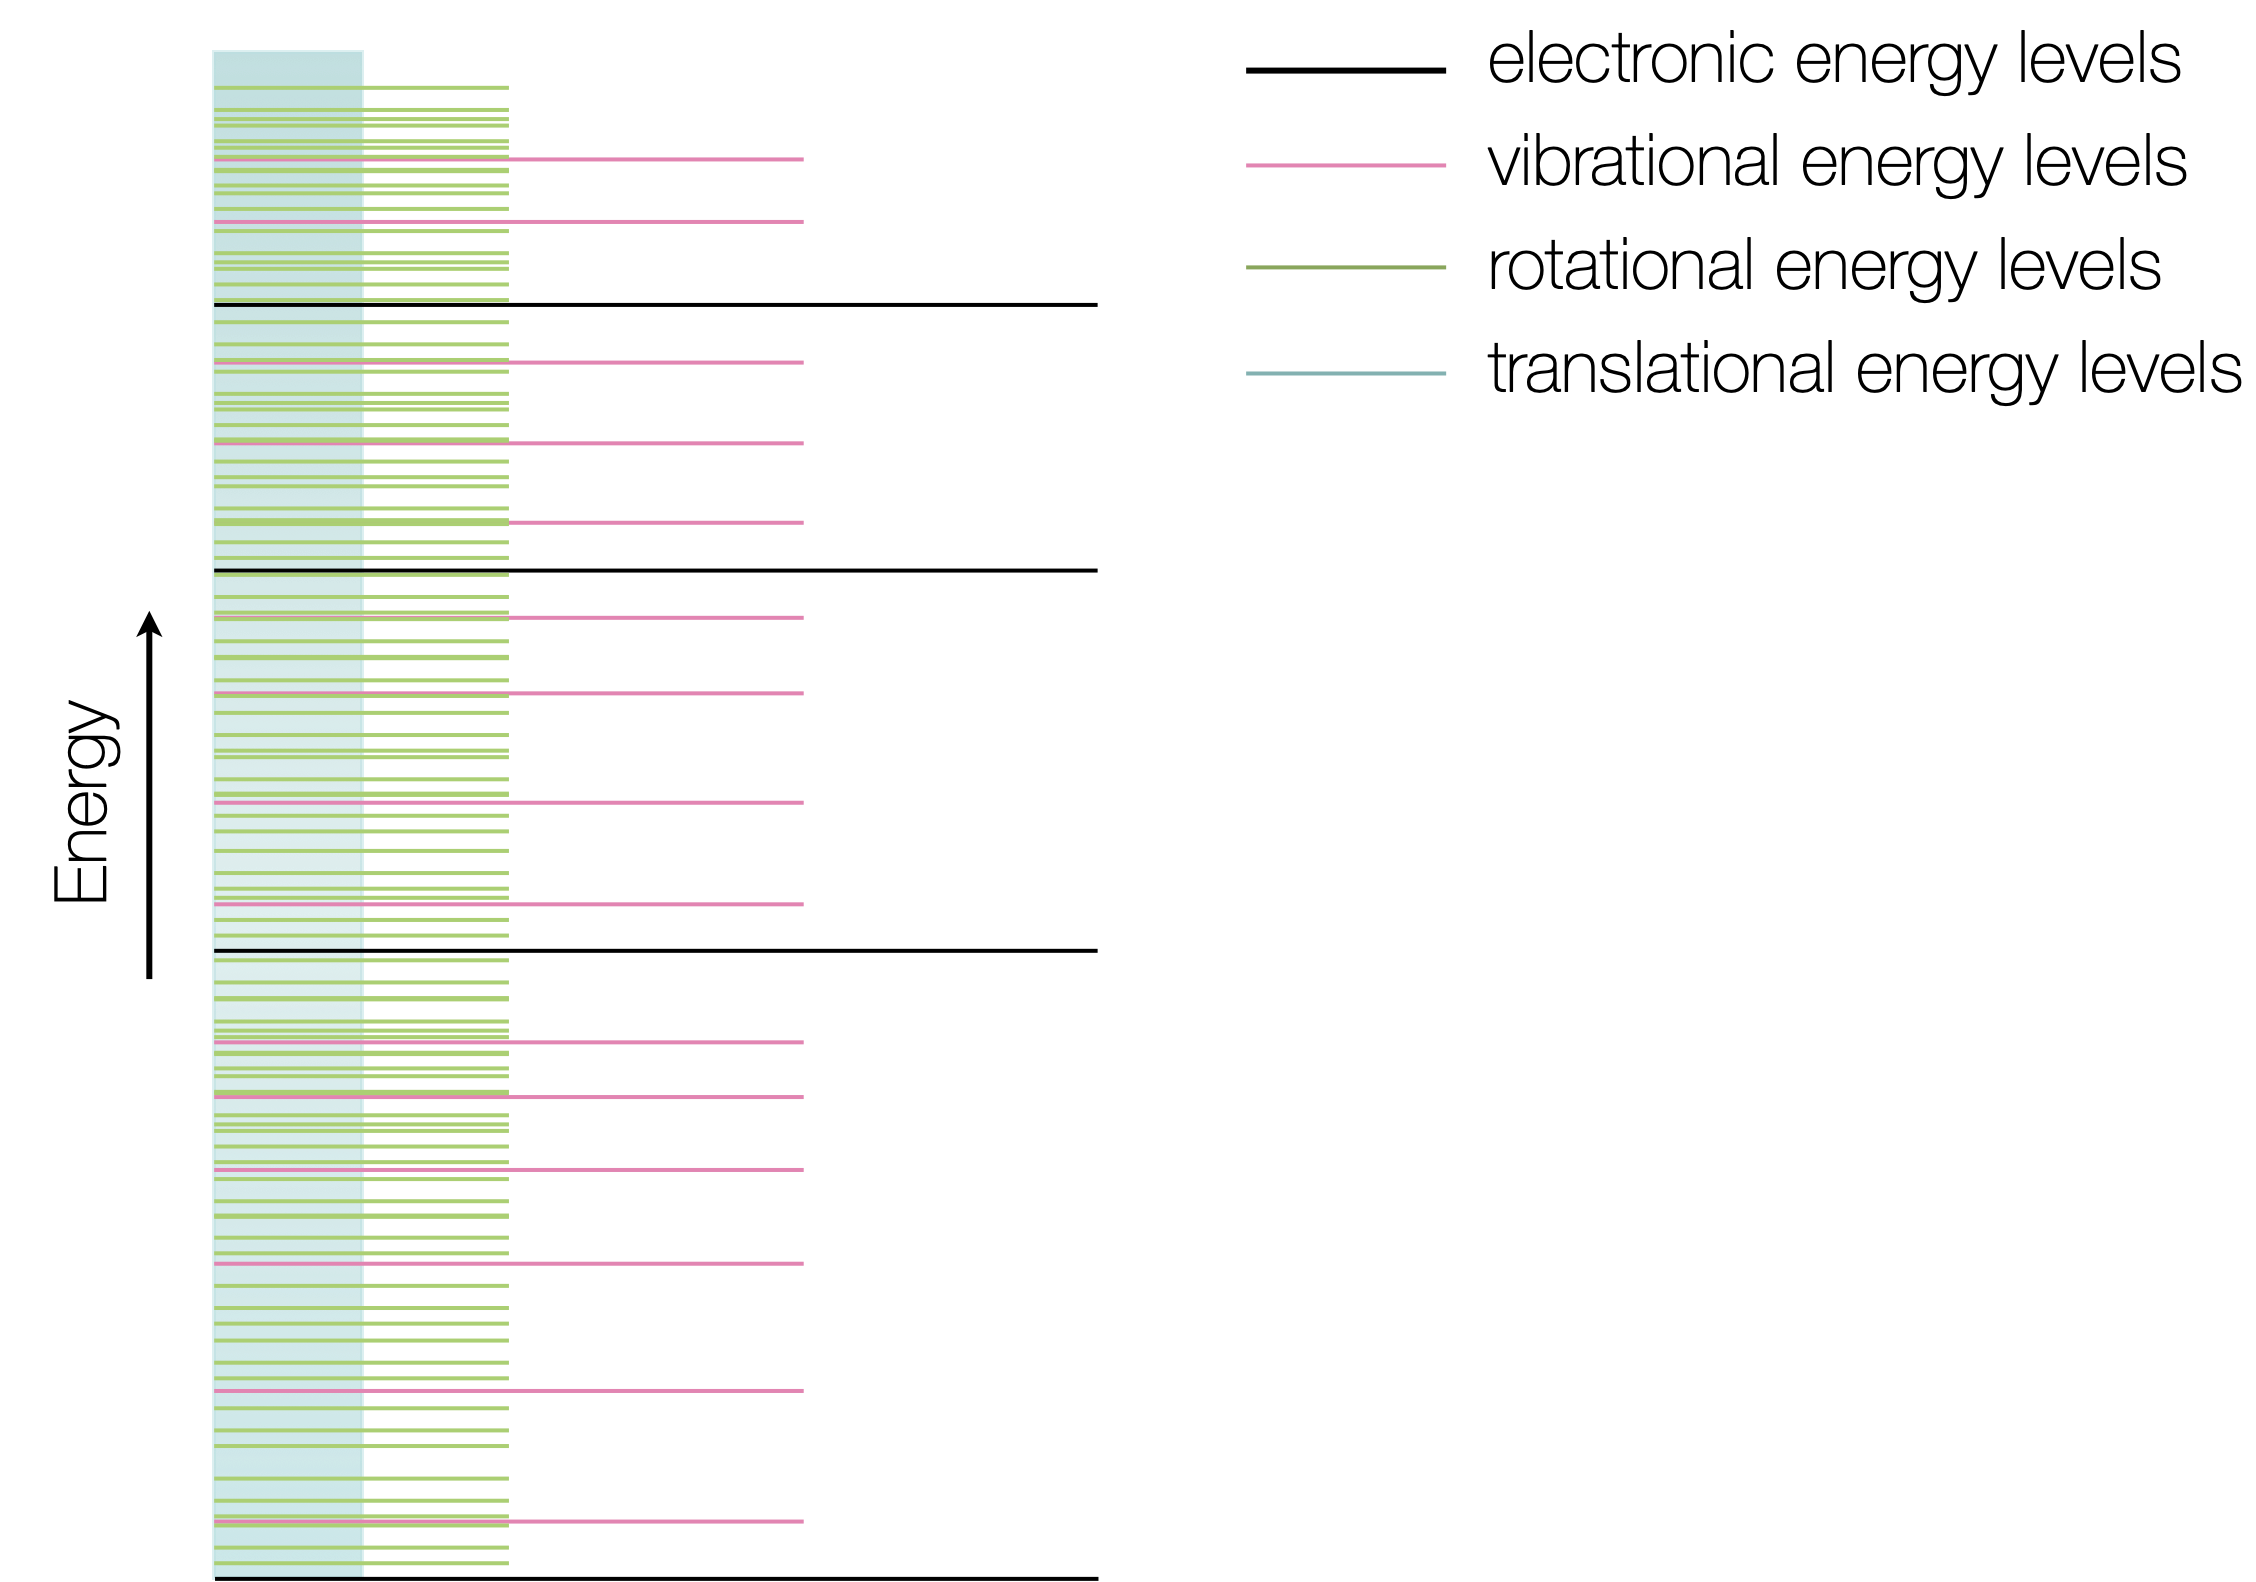
\includegraphics[width=0.8\linewidth]{images/energylevels} 

}

\caption{The energy levels within molecules have different gaps between levels, translational levels are very closely spaced, rotational energy levels have the next closest spacing, vibrational levels are higher in energy still, finally electronic levels have the largest energy gaps.}\label{fig:energylevels}
\end{figure}

The relative populations of these energy levels is given by the Maxwell-Boltzmann equation:

\begin{equation}
\frac{N_i}{N_j}=\frac{g_i}{g_j} \textrm{e}^{-\frac{\Delta E}{k_B T}}
\label{eq:maxwell}
\end{equation}

Looking at equation \eqref{eq:maxwell} we can see that the relative population of energy levels depends upon ΔE, the energy gap between them. This means that the closely spaced translational energy levels are well populated and the particles have a range of speeds associated with this.

At very low temperatures only translational levels are populated, but as the temperature increases and the energy is distributed over more levels rotational levels are then populated, then finally vibrational, at room temperature only there is only a negligible probability of vibrational energy levels being populated.

\begin{figure}

{\centering 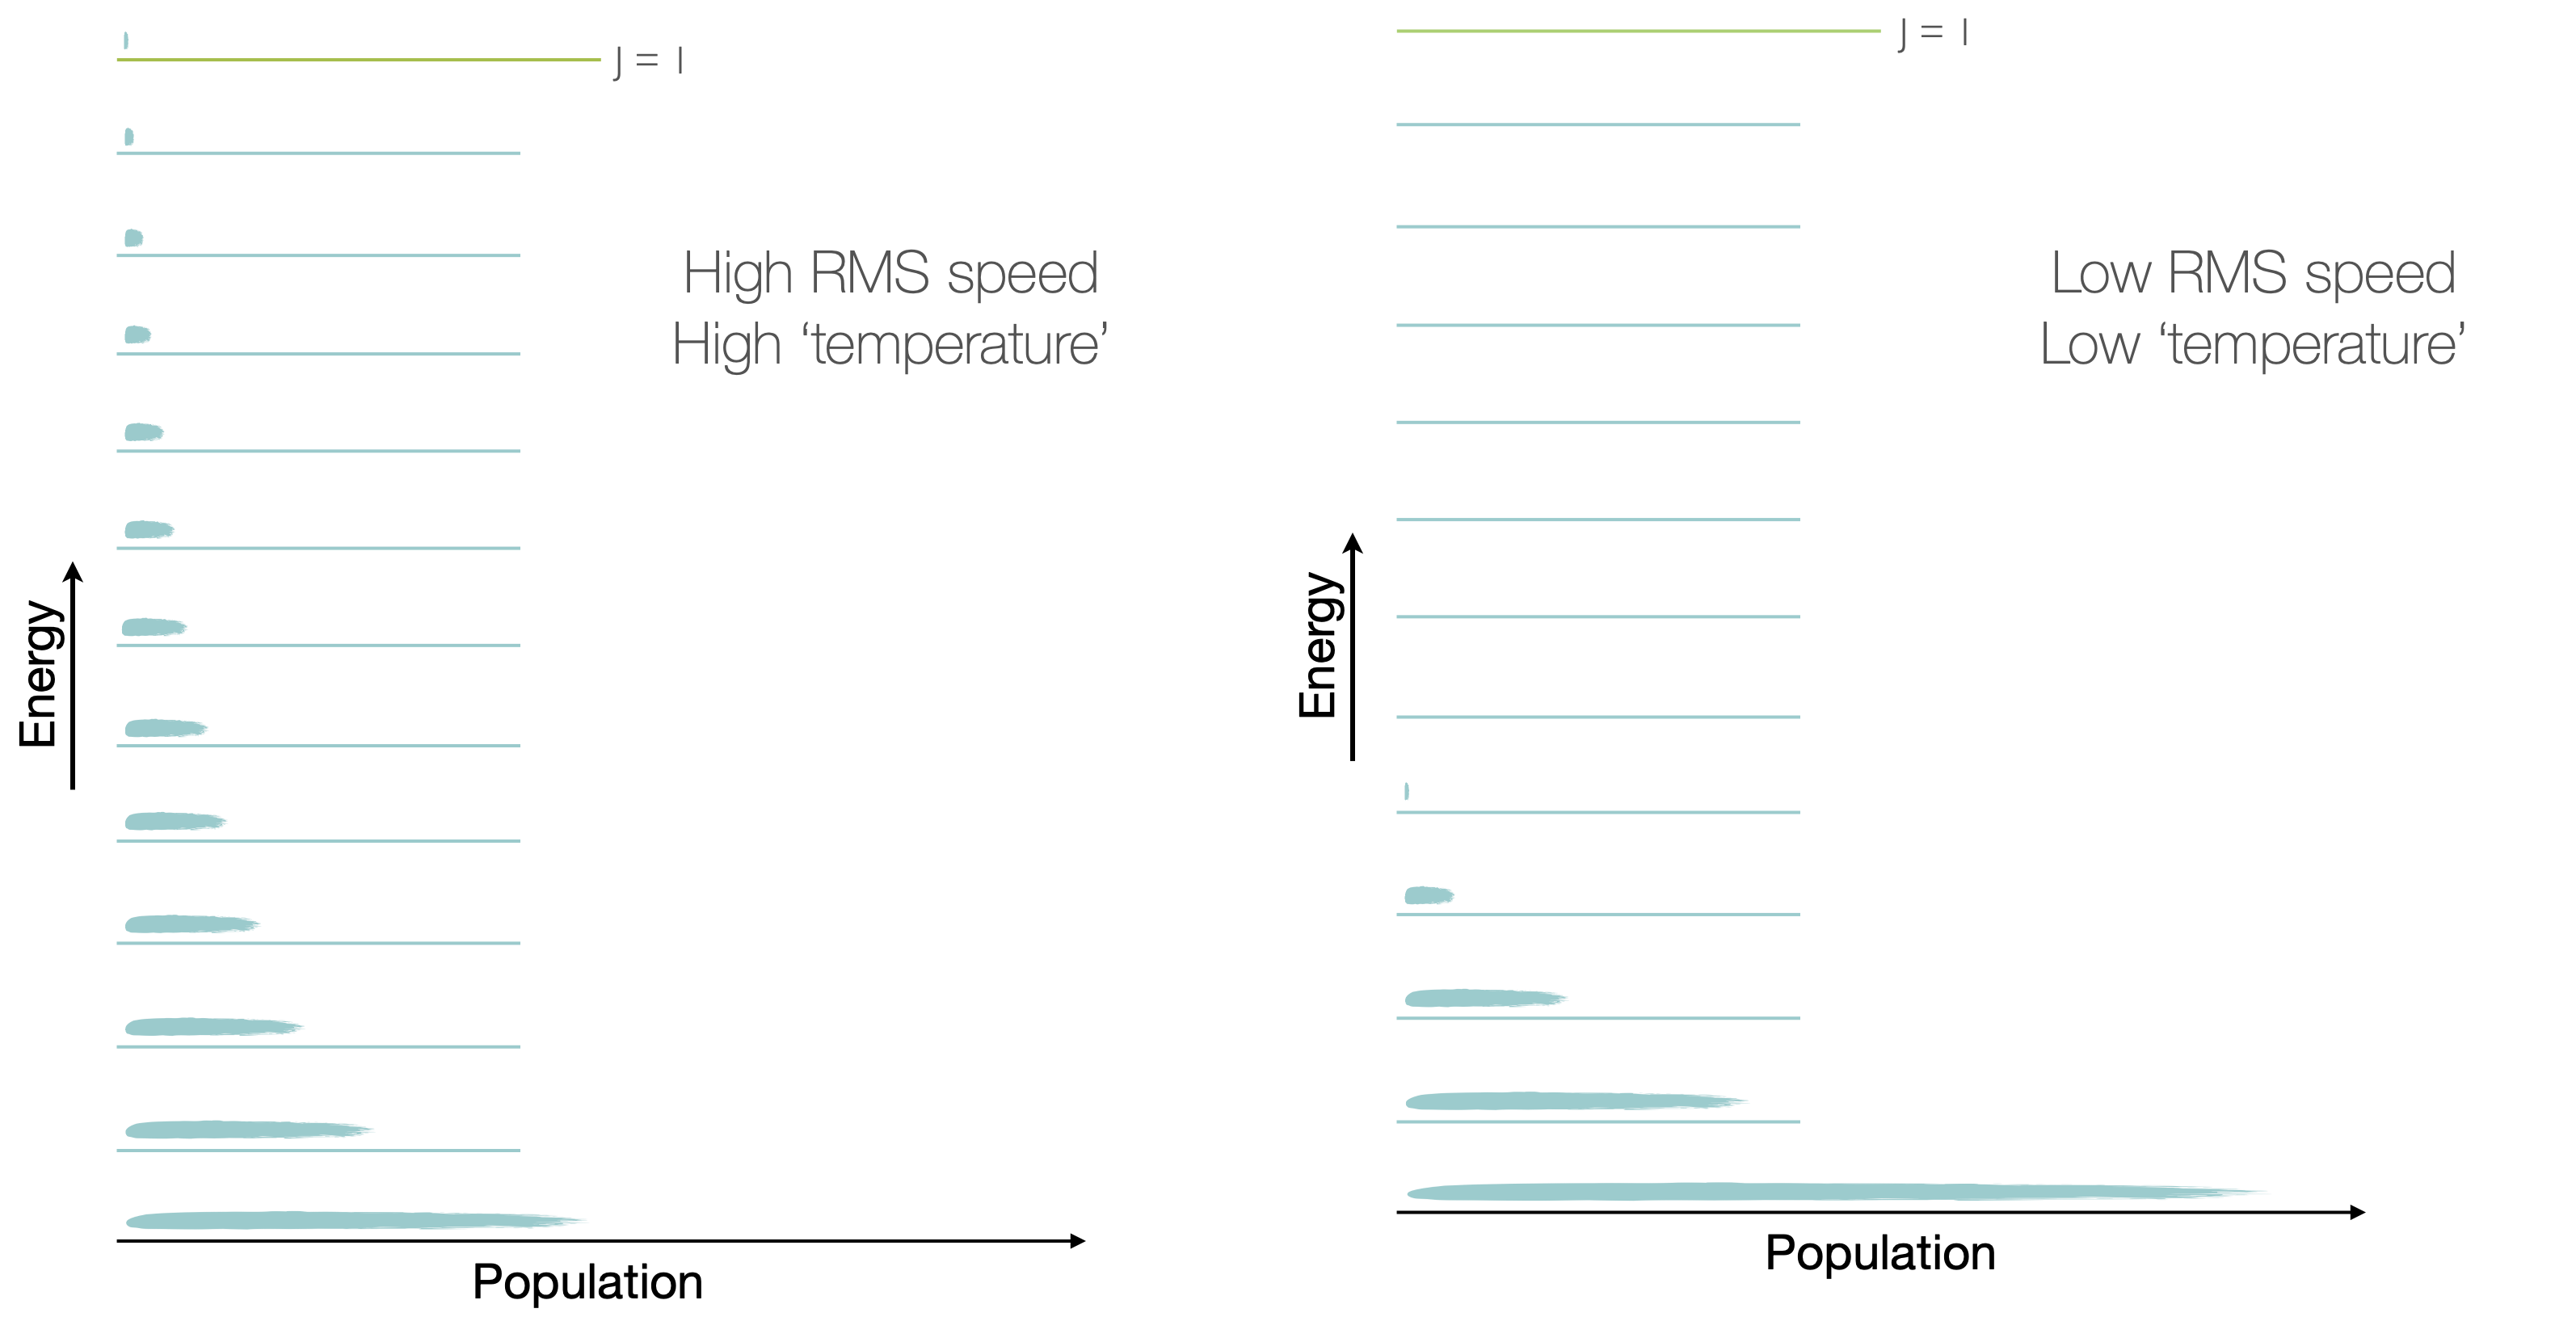
\includegraphics[width=0.8\linewidth]{images/approachingzero} 

}

\caption{As the temperature is decreased the probability of finding particles in the ground translational state increases. At absolute zero all molecules will be in the ground translational state. }\label{fig:approachingzero}
\end{figure}

Therefore temperature is a measure of the population of energy levels within a molecule.

\hypertarget{internal-energy-u}{%
\section{Internal energy, U}\label{internal-energy-u}}

Internal energy is a state function (equation \eqref{eq:internal}), which describes the `total internal energy' of a system. We are already aware that there is thermal energy within the system from the population of the energy levels as described in figure \ref{fig:energylevels}. However internal energy also accounts for the `potential energy' from the inter- and intra- molecular interactions between particles in the system (figure \ref{fig:internalenergy}).

\begin{figure}

{\centering 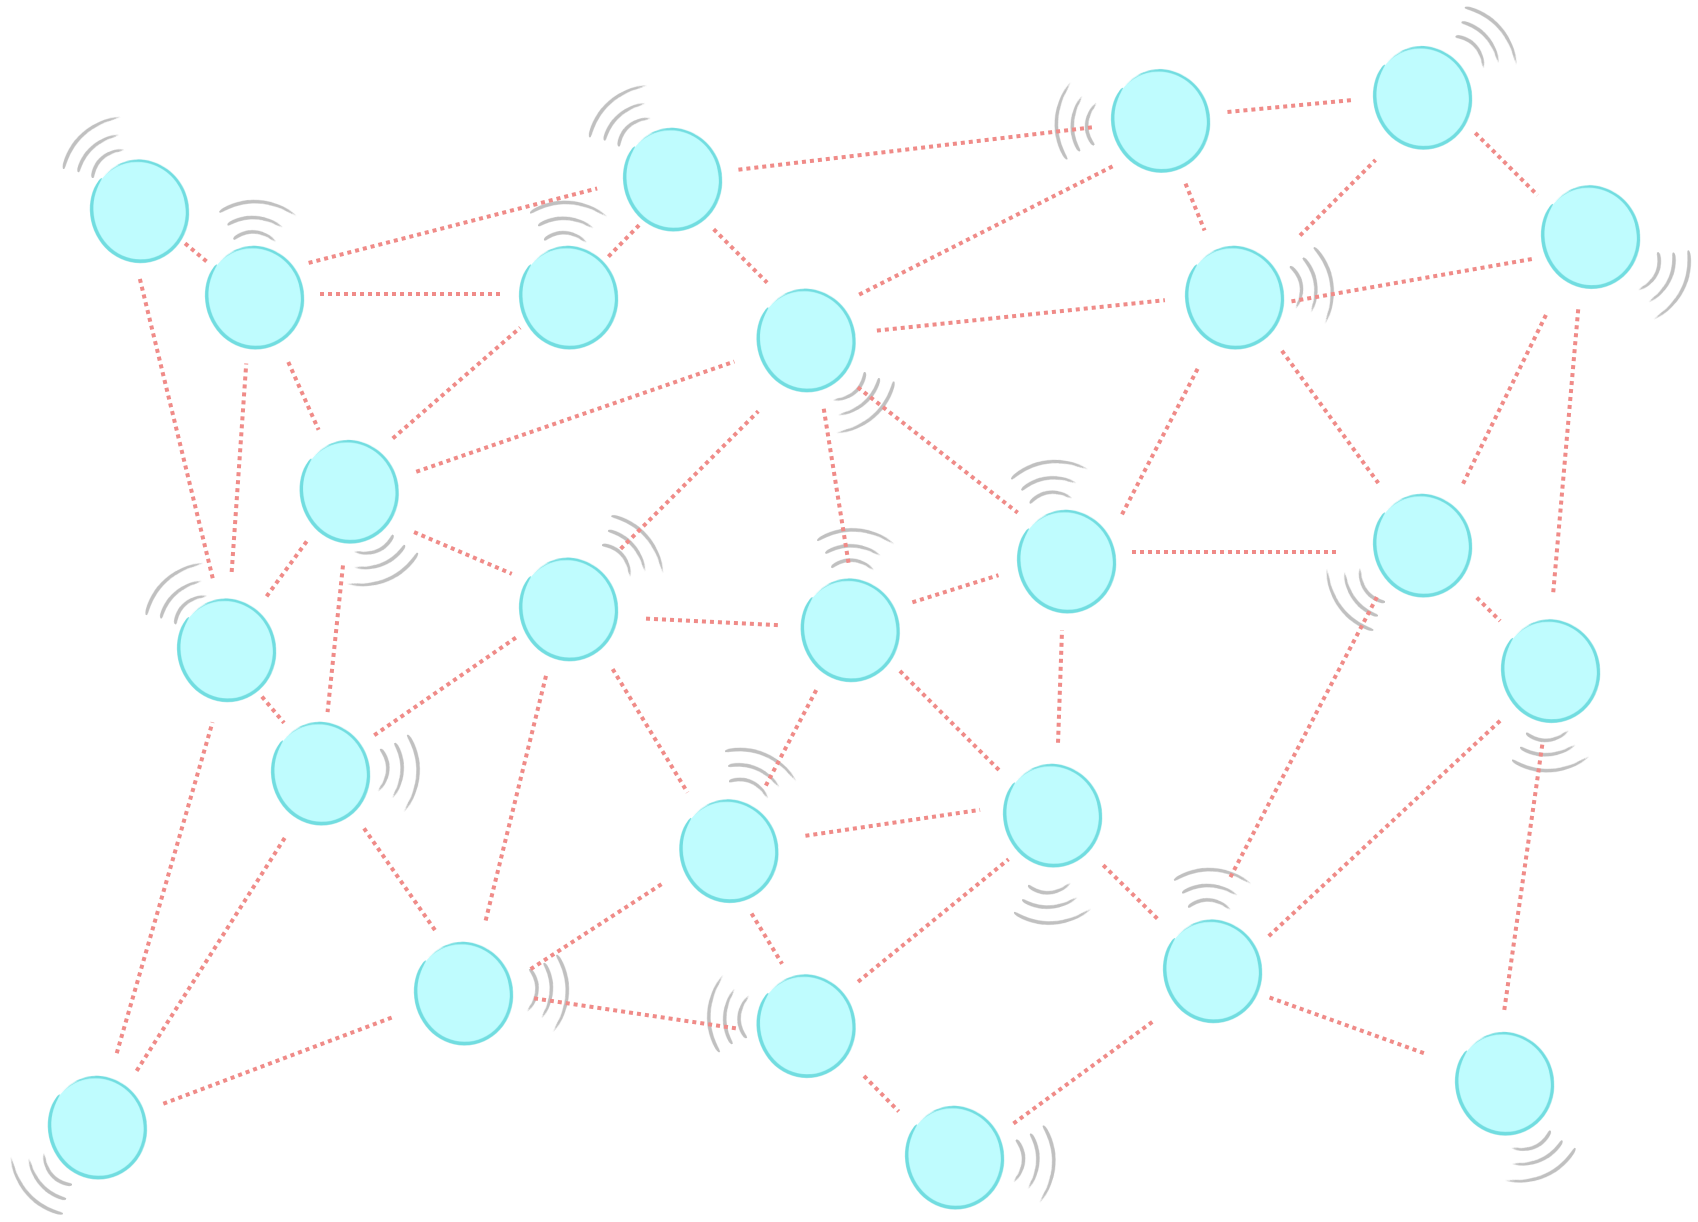
\includegraphics[width=0.8\linewidth]{images/internalenergy} 

}

\caption{The internal energy of a system is the sum of the kinetic and potential energies of the particles in the system.}\label{fig:internalenergy}
\end{figure}

Since internal energy is a state function the change in internal energy in a process is given by the difference in internal energy of the final and initial states (equation \eqref{eq:internal}).

\begin{equation}
\Delta U = U_\textrm{f} - U_\textrm{i}
\label{eq:internal}
\end{equation}

\hypertarget{subsec:equipartition}{%
\subsection{Equipartition theory}\label{subsec:equipartition}}

\emph{Some of the material covered in this video relates to heat capacities which we will study in more detail later in the course.}

Equipartition theory is quite involved, and I am not going to explain any of the actual theory or derivation in this course, instead we are going to just use the results of this theory.

These results from statistical thermodynamic calculation, are verified by emperical observations which is proof of the power of Boltzmann's theories.

Equipartition theory says that for an ideal gas each degree of freedom (section \ref{sec:degreesoffreedom}) contributes \(\frac{RT}{2}\) to the molar internal energy, and so for monatomic gases, such as helium and neon the internal energy , U is \(\frac{3RT}{2}\). However for a diatomic gas with 6 degrees of freedom (3 translational, 2 rotational and 1 vibrational) the internal energy of the ideal gas is predicted to be \(3RT\).

However, we have already seen that the energy spacing between different types of energy level differs, and so only \emph{active} degrees of freedom contribute to the internal energy. Consequently because there are large energy gaps for vibrational energy levels the excited states of these energy levels are rarely occupied and so they do not contribute towards the total internal energy of the system.

\hypertarget{first-law-of-thermodynamics}{%
\section{First Law of Thermodynamics}\label{first-law-of-thermodynamics}}

There are a number of variations on the statements of the first law of thermodynamics, but ultimately they are all saying the same thing. The variations come from different definitions referring to different types of thermodynamic system (Section \ref{sec:typesofsystem}).

The first statement of the first law of thermodynamics is the most fundamental:

\emph{`the internal energy of an isolated system is constant'}

This should be fairly obvious, if my system is isolated there can be no exchange of matter or energy and so the internal energy can't change.

A second version of first law refers to a closed system, one where there can be no exchange of matter, but energy may be exchanged in the form of either heat or work. Mathematically this statement is (\eqref{eq:firstlaw}):

\begin{equation}
\Delta U = q + w
\label{eq:firstlaw}
\end{equation}

where \(q\) is the energy exchanged in the form of heat and \(w\) the energy exchanged in the form of work.

\hypertarget{questions}{%
\section{Questions}\label{questions}}

\begin{enumerate}
\def\labelenumi{\arabic{enumi}.}
\tightlist
\item
  Determine the number of degrees of freedom in each of the following molecules, and consequently predict the molar internal energy at 25 ºC.
\end{enumerate}

\begin{enumerate}
\def\labelenumi{\alph{enumi}.}
\tightlist
\item
  molecular nitrogen, N\textsubscript{2}
\item
  ozone, O\textsubscript{3}
\item
  acetylene HCCH
\end{enumerate}

\begin{enumerate}
\def\labelenumi{\arabic{enumi}.}
\setcounter{enumi}{1}
\item
  Why can't you use equipartition theory to determine the internal energy of ethanol at room temperature?
\item
  If a system looses 250 J of energy from loss of heat, and 600 J of energy is added to the system in the form of work what is the change in internal energy of the system, and the universe?
\item
  How does changing the spacing of energy levels change the distribution of population of energy levels in a system?
\end{enumerate}

\hypertarget{answers}{%
\section{Answers}\label{answers}}

\begin{enumerate}
\def\labelenumi{\arabic{enumi}.}
\item
  \begin{itemize}
  \item
  \end{itemize}
\end{enumerate}

\begin{enumerate}
\def\labelenumi{\alph{enumi}.}
\tightlist
\item
  6.194 kJ mol\textsuperscript{−1}
\item
  7.433 kJ mol\textsuperscript{−1}
\item
  6.194 kJ mol\textsuperscript{−1}
\end{enumerate}

\begin{enumerate}
\def\labelenumi{\arabic{enumi}.}
\setcounter{enumi}{1}
\item
  It's a liquid at room temperature, equipartition theory tells us about ideal gases.
\item
  \(\Delta U_{system}=\) +350 J, \(\Delta U_{universe}=\) 0J
\item
  It shouldn't they will re-space, so if the population of levels is higher when the space is bigger, but you are just distributing the energy differently.
\end{enumerate}

\hypertarget{ch:Part3}{%
\chapter{Week 2 - Part 1}\label{ch:Part3}}

Previously we have been introduced to the concepts of temperature and internal energy, two fundamental concepts in thermodynamics, and we finished by introducing the first law of thermodynamics, and introducing the terms `heat' and `work'. In this part we learn what heat and work are thermodynamically, and extend our idea of state functions to bring the well known concept of Hess' Law to this course.

The unit of energy is joule, this is named after one of the pioneers of thermodynamics.

\emph{The following video has been added for some context to the material, it is not core to the course and the material in it is not examinable.}

\hypertarget{sec:work}{%
\section{Work, w}\label{sec:work}}

In thermodynamics the term `work' describes a mode of transfer of energy between the system and surroundings, this transfer of energy achieves a uniform motion. Work is sometimes considered to be useful energy because this uniform motion may be used to move a piston, lift a weight in a gravitational field or power a phone.

\begin{figure}

{\centering 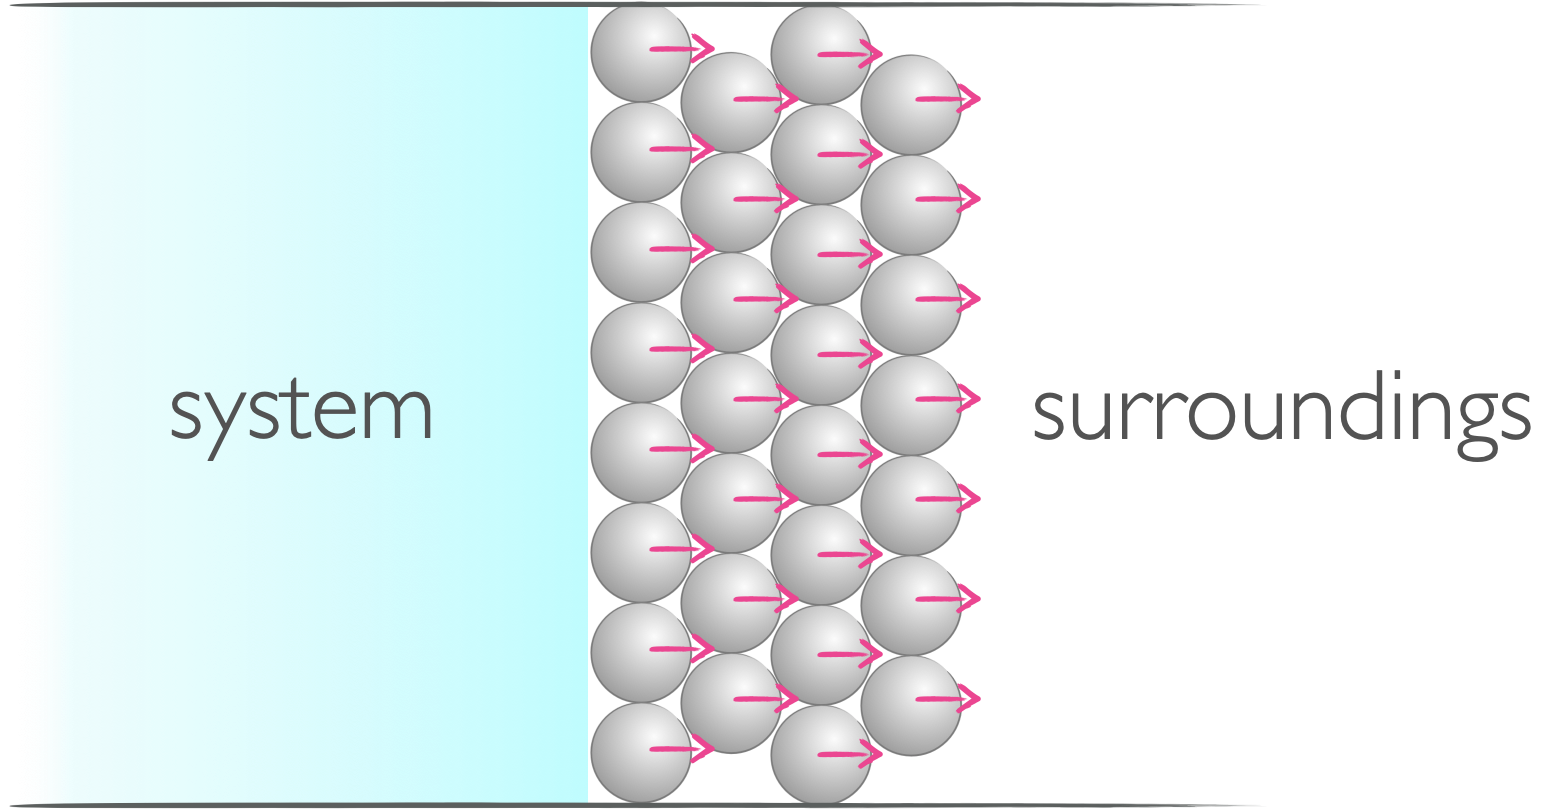
\includegraphics[width=0.5\linewidth]{images/work} 

}

\caption{When energy is transfered in the form of work there is a uniform change in the system or surroundings.}\label{fig:work}
\end{figure}

If we consider the expansion of a gas in a piston against a constant external pressure the gas will expand until the pressure inside and outside of the piston are the same (figure \ref{fig:irrevexpansion}). The work done in this process is given by equation \eqref{eq:irrevexpansion}, and shown as the shaded area in figure \ref{fig:irrevexpansion}.

\begin{figure}

{\centering 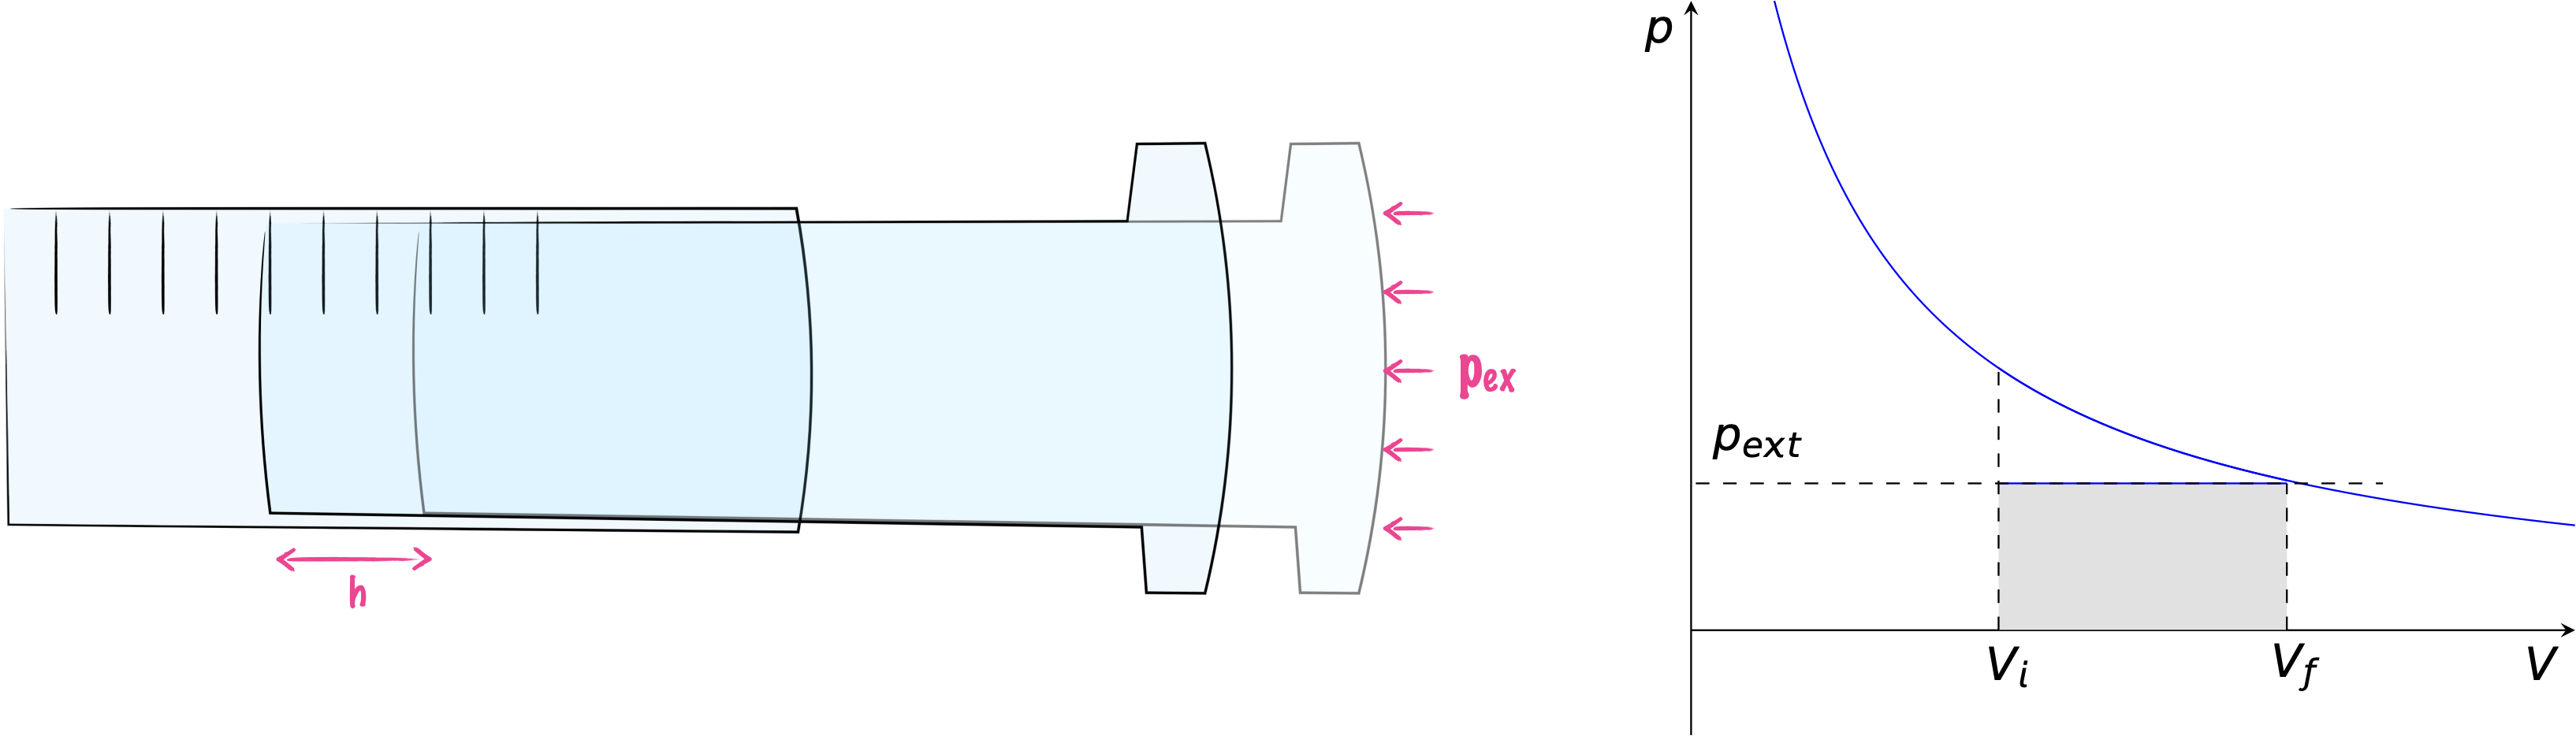
\includegraphics[width=1\linewidth]{images/irrevexpansion} 

}

\caption{If a gas expands against a constant external pressure the expansion will continue until the pressure inside and out of the piston is the same.}\label{fig:irrevexpansion}
\end{figure}

\begin{equation}
w=-p_{\textrm{ex}}\Delta V
\label{eq:irrevexpansion}
\end{equation}

The work done, is negative because if the system does work on the surroundings energy is transferred from the system to the surroundings and the internal energy of the system falls.

You can check the units of this process to help verify this statement, pressure has the units pascal, Pa, which in SI base units is kg m\textsuperscript{−1} s\textsuperscript{−2} and volume of course m\textsuperscript{3}. The units of work are joules, J, which in SI base units is kg m\textsuperscript{2} s\textsuperscript{−2}.

If we instead consider the hypothetical thermodynamically reversible process where the system and surroundings are in equilibrium all through the expansion, this tells us the maximum possible work which can be achieved from a system.

\begin{figure}

{\centering 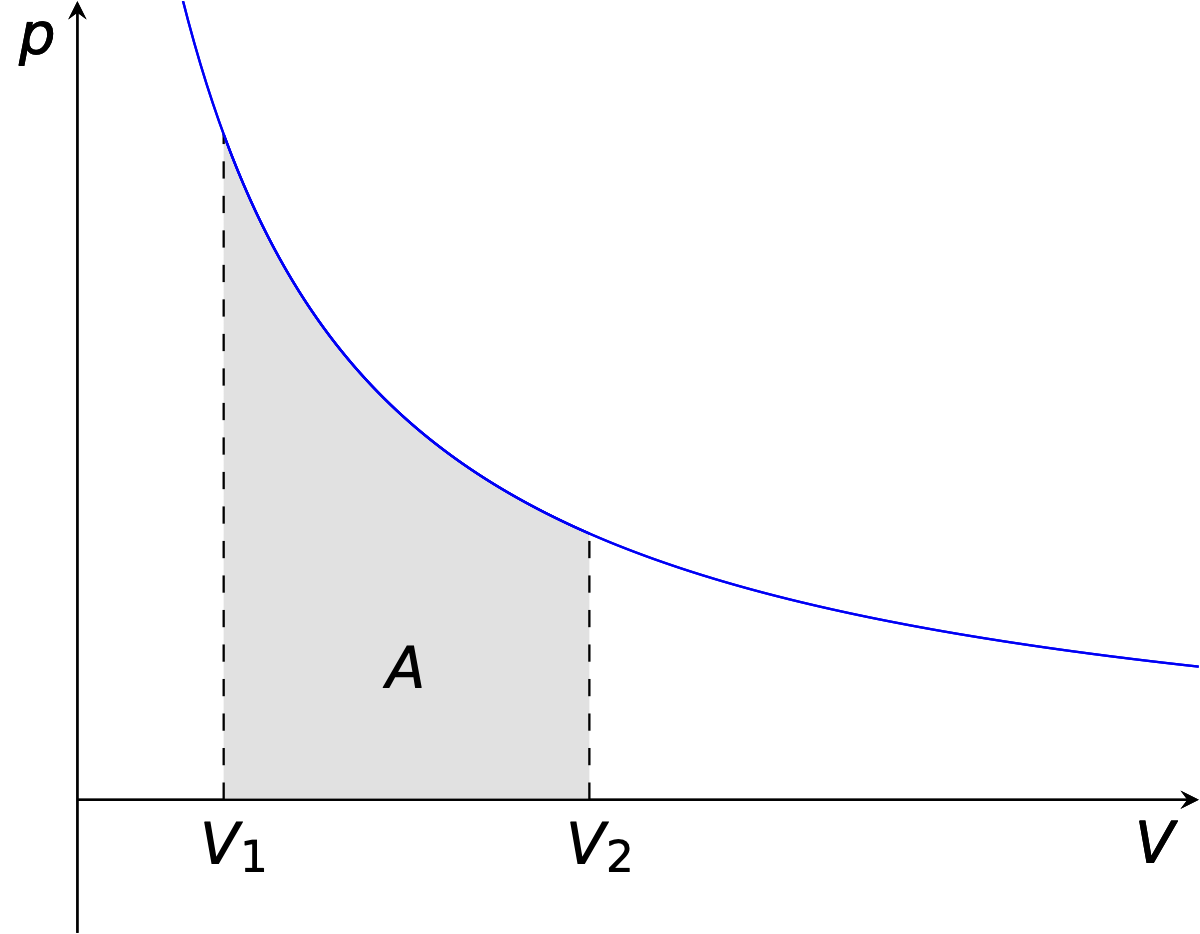
\includegraphics[width=0.5\linewidth]{images/revexpansion} 

}

\caption{If a gas expands and the pressure inside and out are only ever infitessimal difference between the pressure of system and surroundings this is called a reversible expansion and the maximum possible amount of work can be achieved.}\label{fig:revexpansion}
\end{figure}

In the case of a reversible expansion the work done by the system in an expansion is given in equation \eqref{eq:revexpansion}, this expression may be derived from integrating the area under the pV curve in figure \ref{fig:revexpansion}.

\begin{equation}
w=-n\textrm{R}T \ln {\frac{V_\textrm{f}}{V_\textrm{i}}}
\label{eq:revexpansion}
\end{equation}

For the same increase in volume at the temperature of the system increases then the work needed in a reversible expansion also increases.

There are many types of work, but they may all be modeled by expansion work. Other types of work include things like surface expansion, extension of a spring or electrical work.

\hypertarget{sec:heat}{%
\section{Heat, q}\label{sec:heat}}

If you recall the definition of a closed system (section \ref{subsec:closed}), we introduced the concept of energy being able to be exchanged in the form of heat through a diathermic wall, this is just a boundary through which energy in the form of heat may be transferred.

Heat is defined as a mode of transfer of energy that achieves a random motion in the surroundings.

\begin{figure}

{\centering 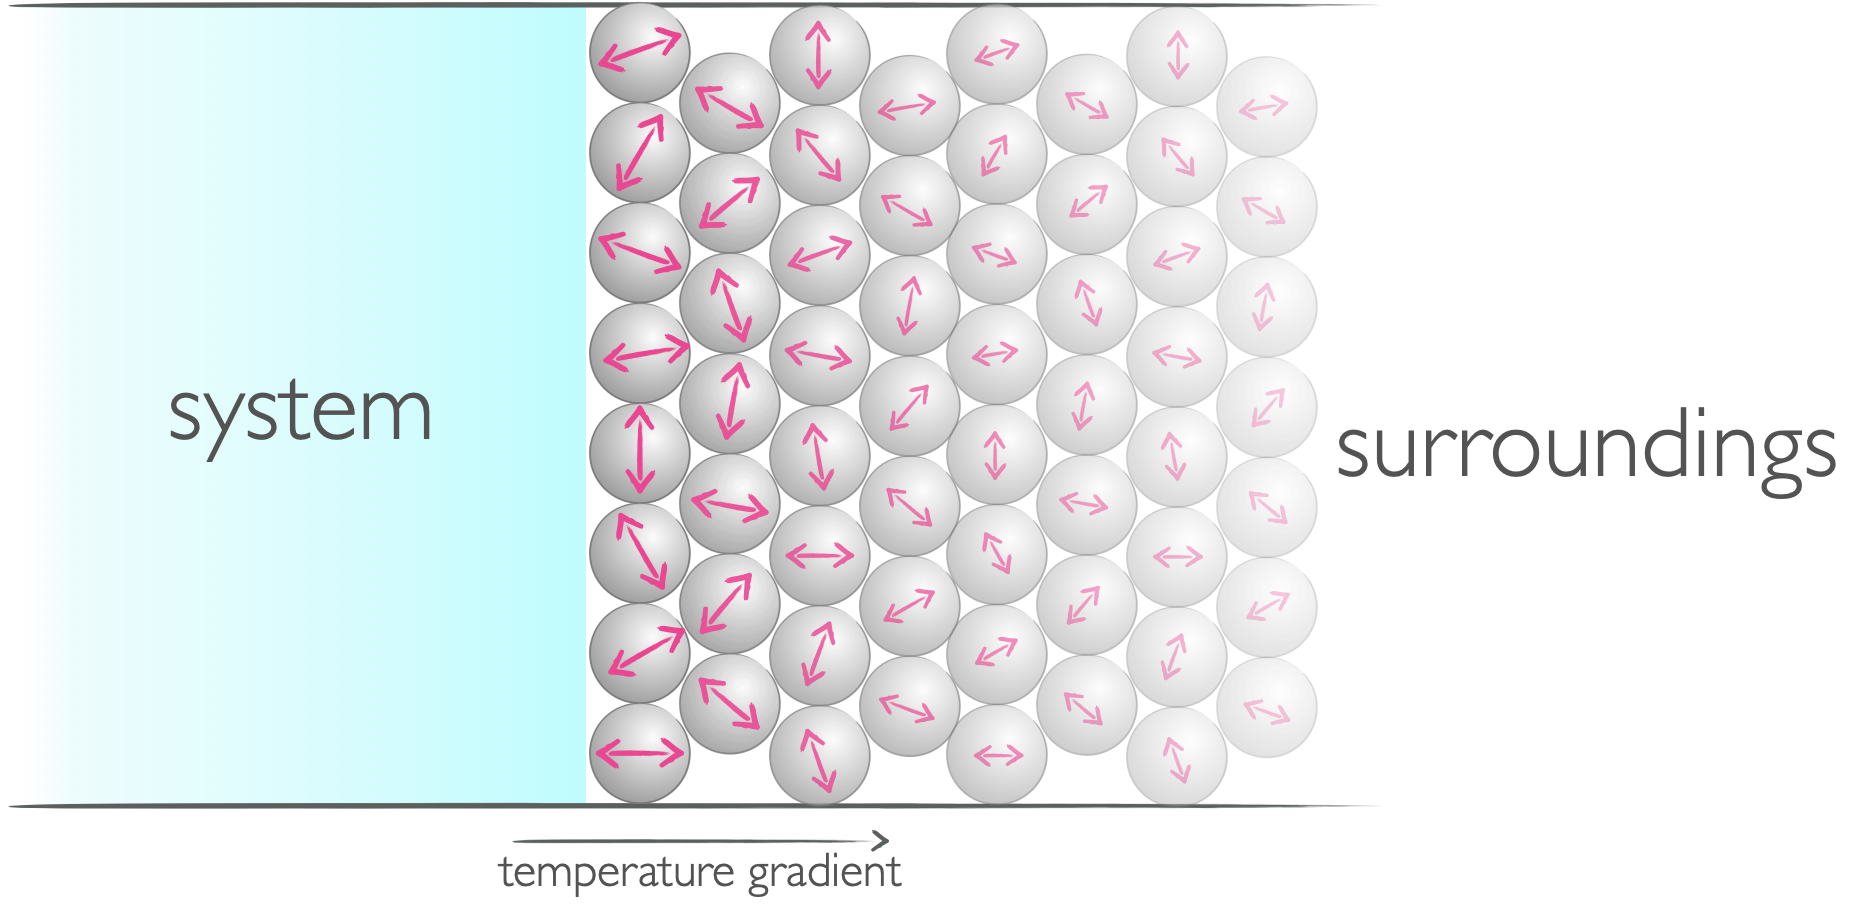
\includegraphics[width=0.5\linewidth]{images/heat} 

}

\caption{When energy is transfered in the form of heat it induces a random motion in the system or surroundings.}\label{fig:heat}
\end{figure}

\begin{itemize}
\item
  When a reaction is exothermic energy in the form of heat is transferred from the system to the surroundings and the internal energy of the system falls (q = -ve).
\item
  When a reaction is endothermic energy in the form of heat is transferred from the surroundings to the system and the internal energy of the system increases (q = +ve).
\end{itemize}

\hypertarget{isothermal-reversible-expansion}{%
\subsection{Isothermal reversible expansion}\label{isothermal-reversible-expansion}}

If a gas is allowed to expand and no heat is transferred then the work done by the system allows the temperature of the system to fall.

\begin{figure}

{\centering 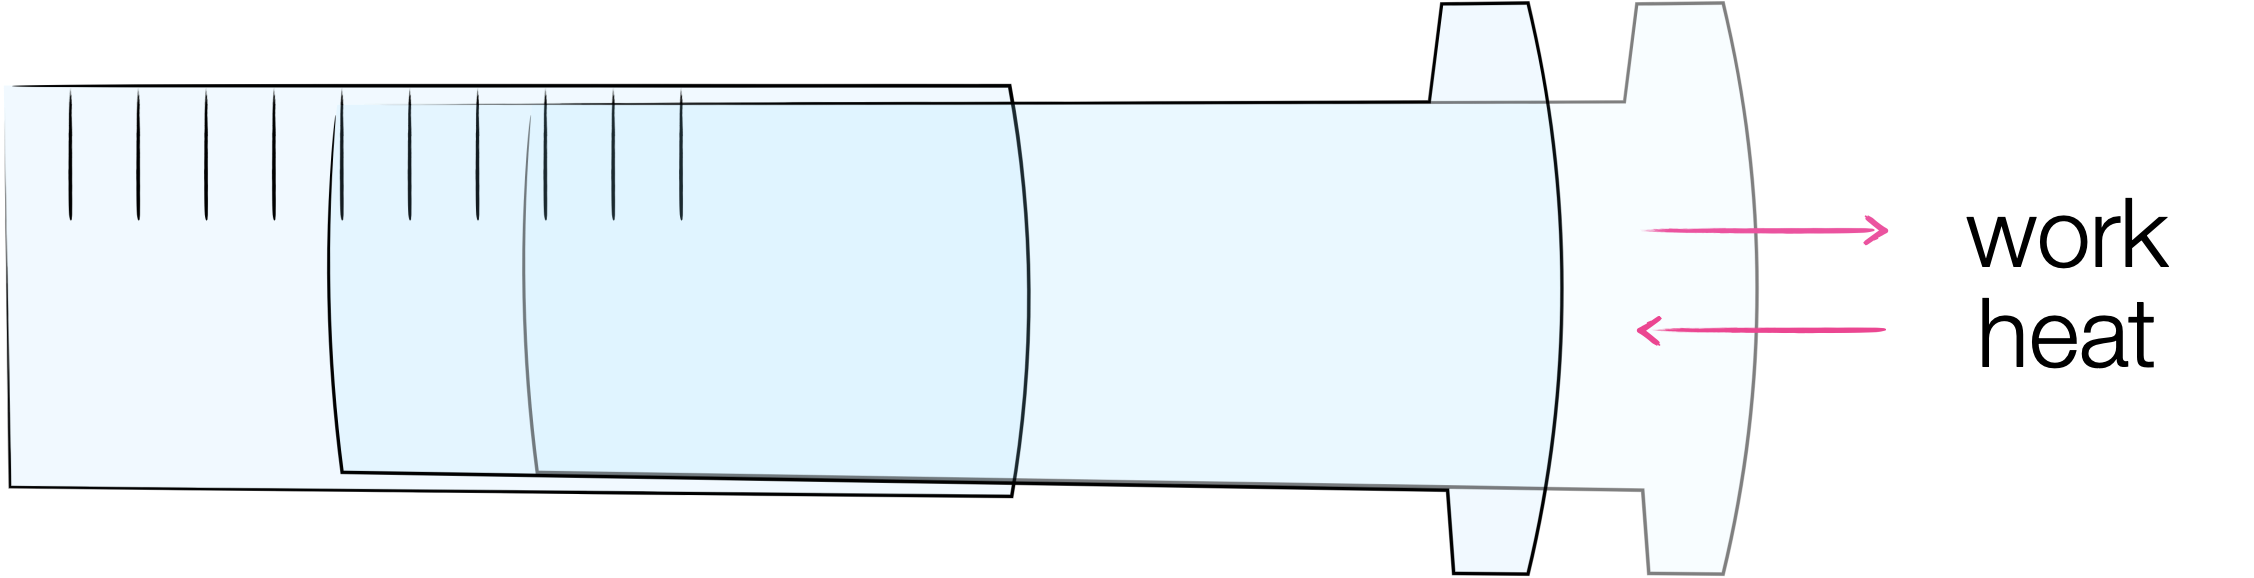
\includegraphics[width=0.5\linewidth]{images/isothermalexpansion} 

}

\caption{In the case of an isothermal reversible expansion the work done by the system and the heat transferred to the system exactly balance.}\label{fig:isothermalexpansion}
\end{figure}

There is a special case where we can consider the expansion of a gas but energy is transferred from the surroundings to the system in the form of heat. In this isothermal reversible expansion the work done by the system is exactly equal and opposite to the heat transferred to the system, and so the net change in internal energy is zero.

Therefore, by applying this to equation \eqref{eq:revexpansion}, we can see for an isothermal reversible expansion:

\begin{equation}
q=n\textrm{R}T \ln {\frac{V_\textrm{f}}{V_\textrm{i}}}
\label{eq:isothermalexpansion}
\end{equation}

This is just an example of the first law of thermodynamics in action.

\hypertarget{enthalpy-h}{%
\section{Enthalpy, H}\label{enthalpy-h}}

The enthalpy of a system is given by:

\begin{equation}
H = U+pV
\label{eq:enthalpy}
\end{equation}

at constant pressure the enthalpy change of a system is given by:

\begin{equation}
\Delta H = \Delta U + p\Delta V
\label{eq:enthalpychange}
\end{equation}

Fundamentally enthalpy is a way of keeping track of internal energy when we are working in systems which are at constant pressure, systems which are allowed to do expansion work against the atmosphere.

If we take both our original definitions of enthalpy and internal energy we can bring enthalpy back to a concept I am sure you are all familiar. That being heat:

\begin{equation*}
\Delta H = \Delta U + p\Delta V
\end{equation*}

and

\begin{equation*}
\Delta U = w + q
\end{equation*}

then

\begin{equation*}
\Delta H = w + q + p \Delta V
\end{equation*}

Therefore:

\begin{equation}
\Delta H_p = q
\label{eq:enthalpyconstp}
\end{equation}

Consequtnly at 25 ºC the molar enthalpy of an ideal gas is about 2.5 kJ mol\textsuperscript{−1}

\hypertarget{hesss-law}{%
\section{Hess's Law}\label{hesss-law}}

Just like internal energy, enthalpy is a state function, and the relationship between the enthalpy of a reaction is just the difference in enthalpy of the final and initial states.

Hess' law (equation \eqref{eq:enthalpystate1})is just application of the nature of enthalpy being a state function:

\begin{equation}
\Delta_r H^{\ominus} = \sum_{products}v \Delta H^{\ominus}_\textrm{X}-\sum_{reactants}v \Delta H^{\ominus}_\textrm{X}
\label{eq:enthalpystate1}
\end{equation}

If the enthalpy of reaction is positive the reaction is endothermic heat is transferred from the surroundings to the system and the temperature of the surroundings falls, if the enthalpy of reaction is negative the reaction is exothermic heat is transferred from the system to the surroundings and the temperature of surroundings increases.

\hypertarget{constant-volume-and-constant-pressure}{%
\subsection{Constant volume and constant pressure}\label{constant-volume-and-constant-pressure}}

This is just to highlight that at constant volume the system cannot expand and therefore no work can be done, consequently \(\Delta U_V = q\).

At constant pressure the work done, \(-p \Delta V\) means that the change in enthalpy (\(\Delta H = \Delta U + p \Delta V\)) is given by \(\Delta H_p=q\).

\hypertarget{questions-1}{%
\section{Questions}\label{questions-1}}

\begin{enumerate}
\def\labelenumi{\arabic{enumi}.}
\item
  When exactly one mole of an ideal gas is `heated' with 1.75 kJ of energy, it expands doing 250 J of work. What is the change in internal energy of the gas?
\item
  Suppose we have two otherwise identical calorimeters, one calorimeter of fixed volume (isochoric) and the other calorimeter of fixed pressure (isobaric). If exactly the same amount of substance was burnt in excess oxygen in each, which would record the highest temperature change in the surroundings?
\end{enumerate}

\begin{itemize}
\tightlist
\item
  it would be the same in each
\item
  the isochoric system
\item
  the isobaric system
\item
  not enough information to determine
\end{itemize}

\begin{enumerate}
\def\labelenumi{\arabic{enumi}.}
\setcounter{enumi}{2}
\item
  For a reaction conducted at constant pressure and at 20.0 ºC the change in the number of moles of gas (\(\Delta n_{gas}\)) is +2. Calculate the difference between \(\Delta H\) \& \(\Delta U\).
\item
  Calculate the standard enthalpy of formation of \(N_2 O_5\) from the following data:
\end{enumerate}

\(2 NO_{(g)} + O_{2(g)} \longrightarrow 2 NO_{2(g)}\) \(\Delta _r H^\ominus = -114.1\) kJ mol\(^{-1}\)

\(4 NO_{2(g)} + O_{2(g)} \longrightarrow 2 N_2 O_{5(g)}\) \(\Delta _r H^\ominus = -110.2\) kJ mol\(^{-1}\)

\(N_{2(g)} + O_{2(g)} \longrightarrow 2 NO_{(g)}\) \(\Delta _r H^\ominus = +180.5\) kJ mol\(^{-1}\)

\begin{enumerate}
\def\labelenumi{\arabic{enumi}.}
\setcounter{enumi}{4}
\item
  Calculate the expansion work done on the system when 9.576 g of solid ammonium chloride, NH\textsubscript{4}Cl, decomposes completely to yield gaseous ammonia, NH\textsubscript{3} and hydrogen chloride, HCl at a temperature of 1,410 K. Treat the expansion as irreversible and the gases formed as perfect.
\item
  What is the maximum amount of work available when 1 mole of a gas doubles in volume at 25 \(^\circ\)C?
\end{enumerate}

\begin{itemize}
\tightlist
\item
  How does this change with increasing temperature?
\item
  If the expansion is isothermal how much heat is added to the system?
\end{itemize}

\hypertarget{answers-1}{%
\section{Answers}\label{answers-1}}

\begin{enumerate}
\def\labelenumi{\arabic{enumi}.}
\item
  \begin{itemize}
  \tightlist
  \item
    1.50 kJ
  \end{itemize}
\item
  not enough infomation to determine, we would need to know if the net change in gas molecules of the system is postive or negative.
\item
  \(\Delta H - \Delta U\) = +4.876 kJ
\item
  \(Δ_fH^\ominus\) = +11.3 kJ mol\textsuperscript{−1} per mole of N\textsubscript{2}O\textsubscript{5}
\item
  w = -4.198 kJ
\item
  w = −1.72 kJ, increases, q= -w = +1.72 kJ.
\end{enumerate}

\hypertarget{ch:Part4}{%
\chapter{Week 2 - Part 2}\label{ch:Part4}}

\hypertarget{heat-capacity-cx}{%
\section{\texorpdfstring{Heat capacity, C\textsubscript{X}}{Heat capacity, CX}}\label{heat-capacity-cx}}

The heat capacity of a material is the amount of energy required to raise the temperature of that material by 1 K, however there are many different versions of heat capacity, covering both extensive an intensive properties.

Perhaps more confusingly when looking at gases we have to consider whether the heat capacity of a material is at constant pressure or constant volume. This is because if we are at consant pressure the gas has to do work in expanding, and so heat capacitites at constant volume are always smaller than those at constant pressure.

Heat capacity varies with temperature, we can usually say values will be constant within about 100 K, but numerous measurements have been used to show that the heat capacity varies with temperature as follows:

\begin{figure}

{\centering 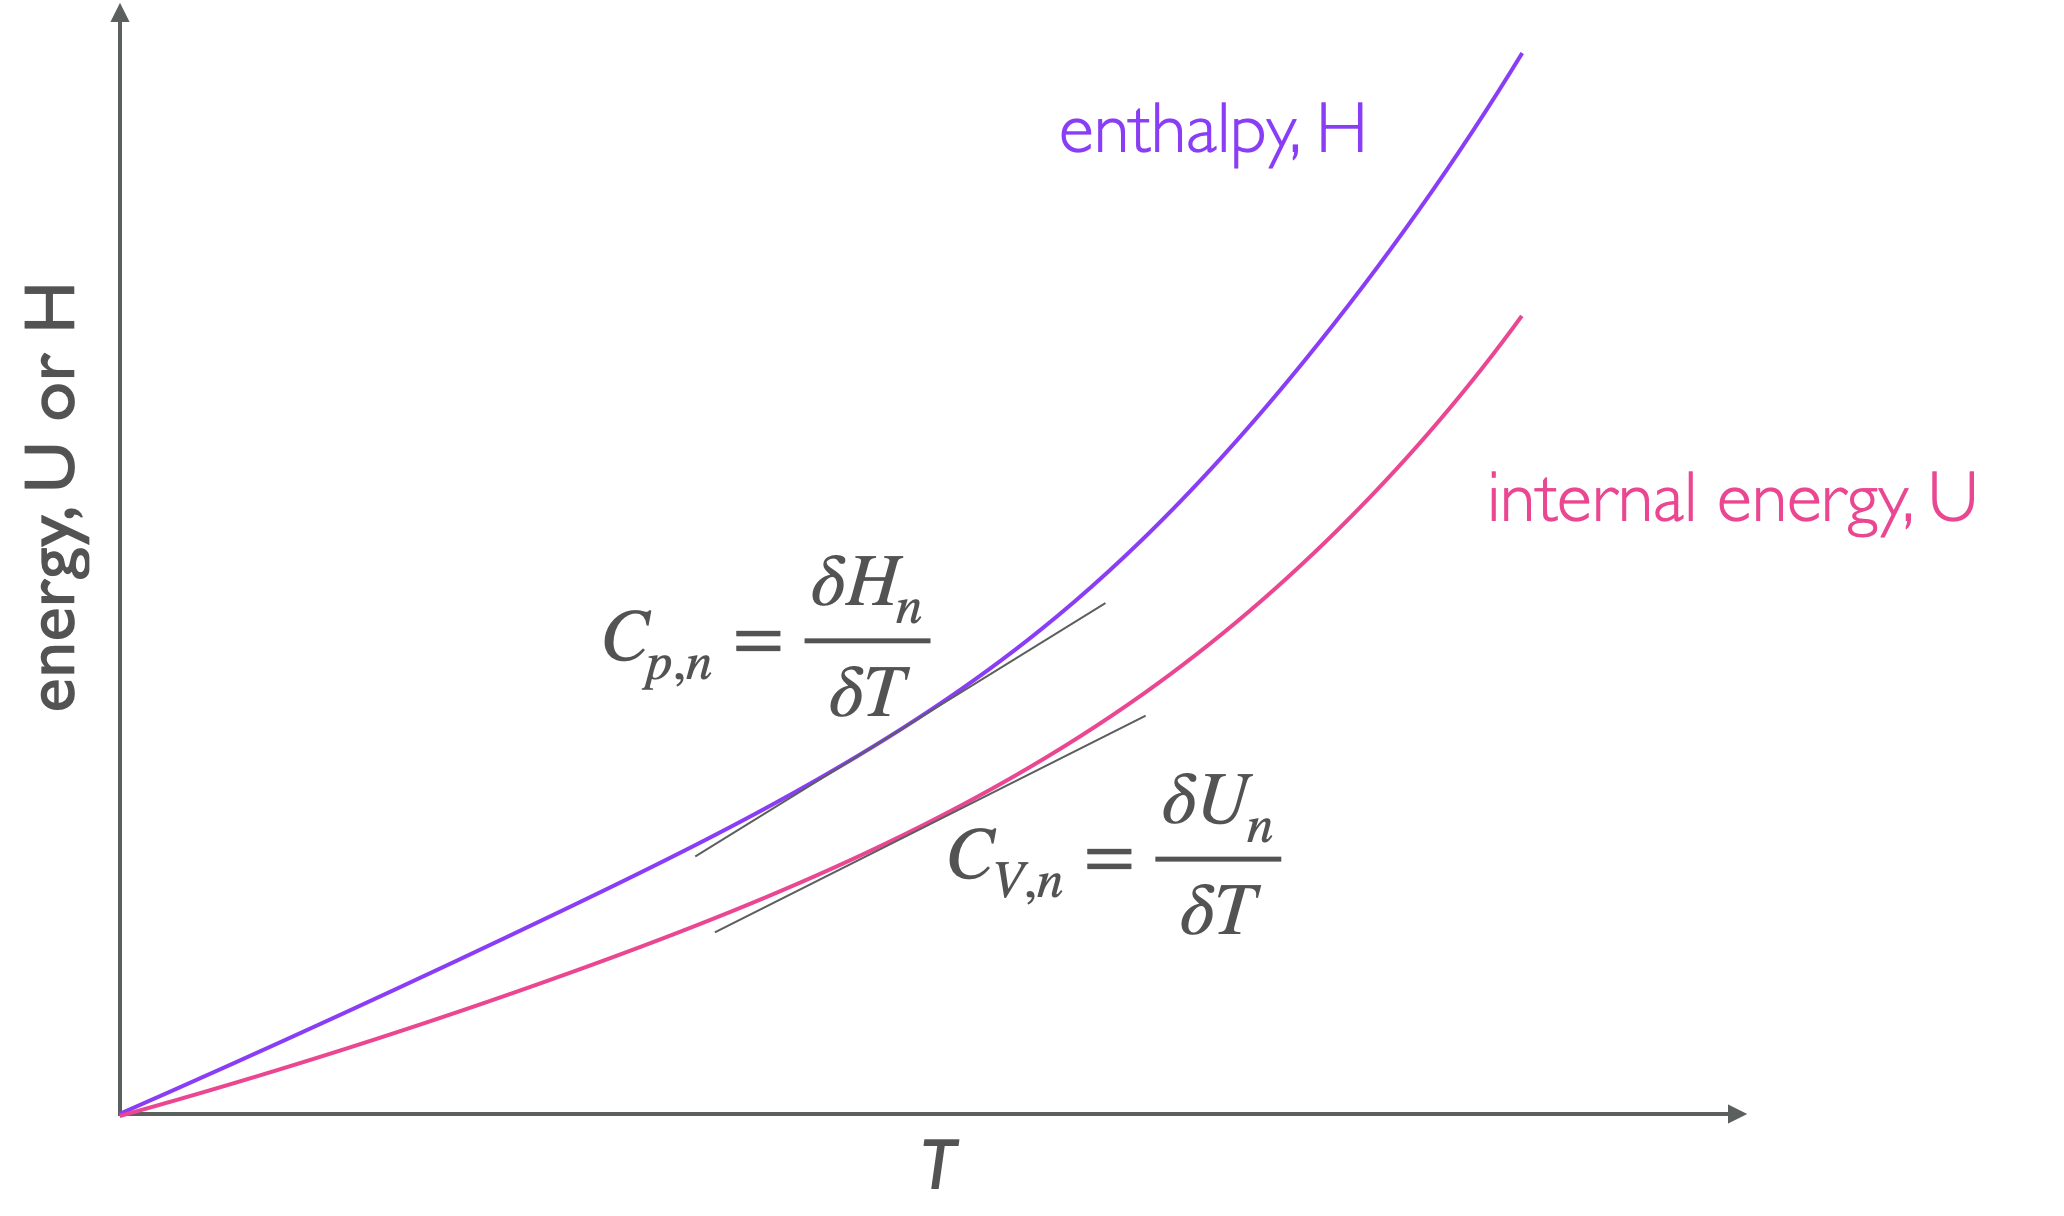
\includegraphics[width=0.7\linewidth]{images/heatcapacitypV} 

}

\caption{The heat capacity of a material is the gradient of the line on an energy verses temperature plot.}\label{fig:heatcapacitypV}
\end{figure}

\begin{equation}
C_{p,n}=\textrm{a}+\textrm{b}T+\frac{\textrm{c}}{T^2}
\label{eq:heatcapacitytemp}
\end{equation}

the constants, a, b and c are measured emperically and are known for a wide range of materials.

Previously in section @ref\{subsec:equipartition\} we have seen how equipartition theory predicts the heat capacity of ideal gases. Like the internal energy only degrees of freedom which are active contribute to heat capacity of a material, and this consideration needs to be made.

\begin{itemize}
\item
  Every translational degree of freedom contributes \(\frac{1}{2}R\) to the heat capacity
\item
  Every rotational degree of freedom contributes \(\frac{1}{2}R\) to the heat capacity
\item
  Every vibrational degree of freedom contributes \(R\) to the heat capacity
\end{itemize}

We can see the heat capacity of molecules changing as the different degrees of freedom are activated.

\begin{figure}

{\centering 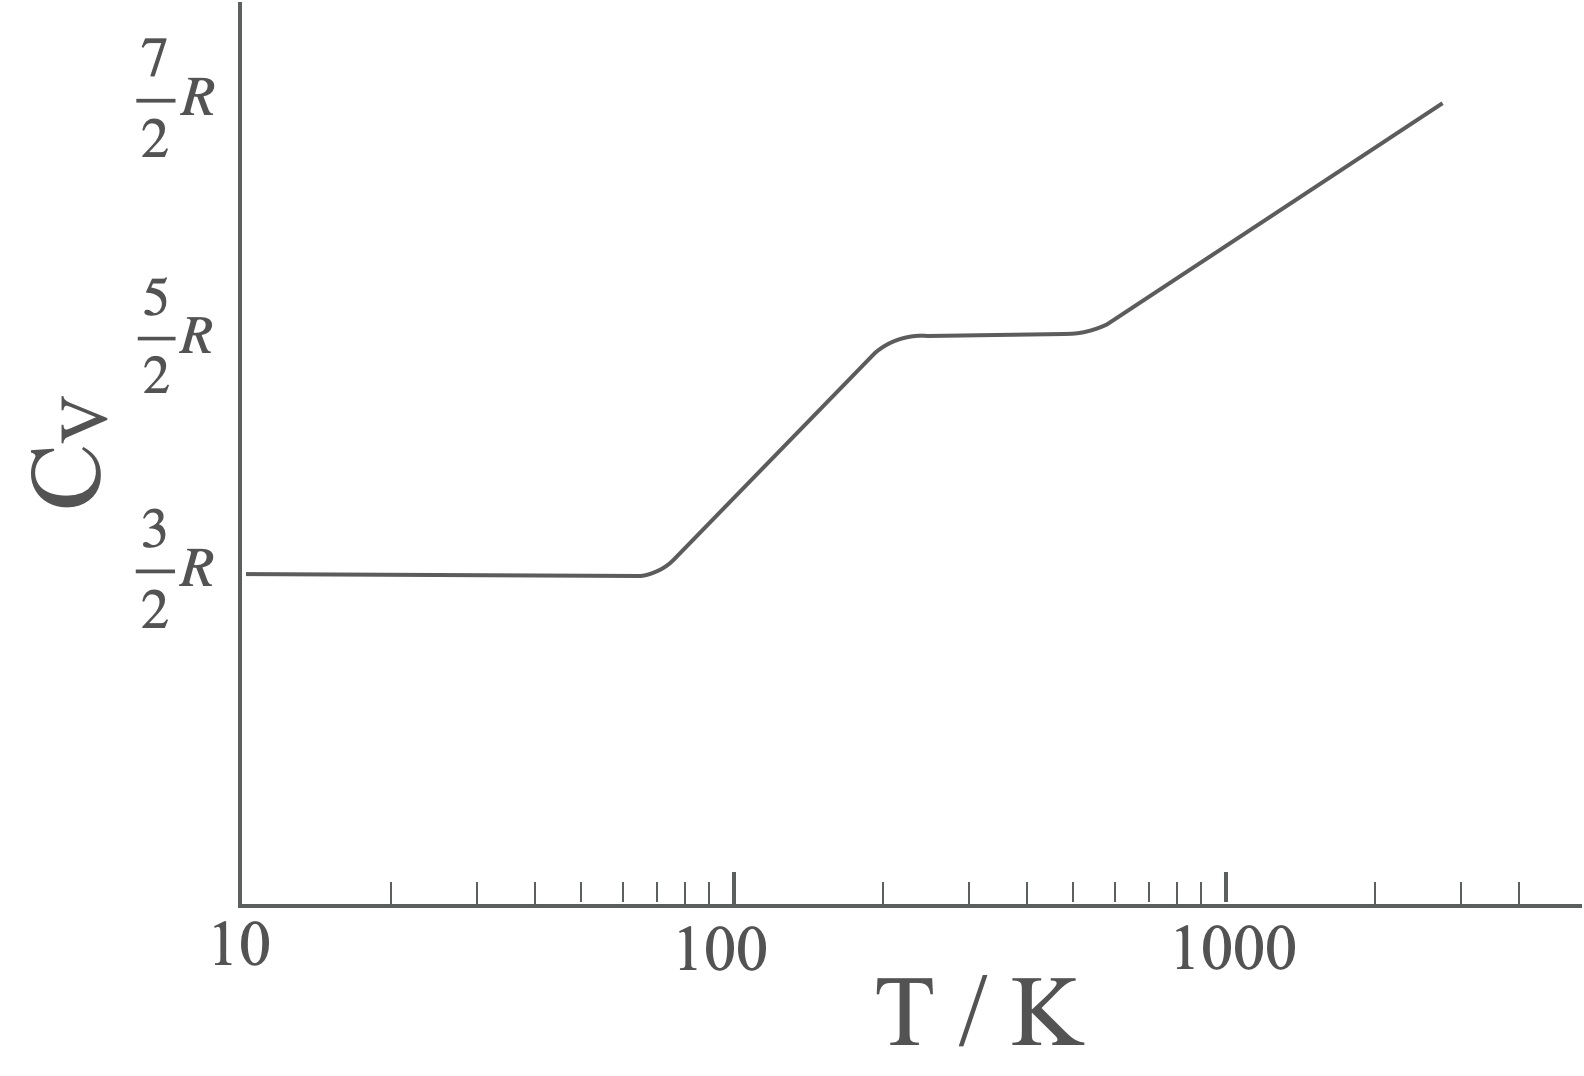
\includegraphics[width=0.7\linewidth]{images/H2heatcapacity} 

}

\caption{The heat capacity of molecular hydrogen varies with temperature, showing clear steps as each type of degree of freedom are activated. At very high temperatures dissociation occurs before the final plateau is observed.}\label{fig:H2heatcapacity}
\end{figure}

\hypertarget{temperature-dependance-of-enthalpy}{%
\section{Temperature dependance of enthalpy}\label{temperature-dependance-of-enthalpy}}

The enthalpy of reaction is dependent upon the temperature of reaction (figure \ref{fig:enthalpytemp}), the relationship between the enthalpies at two tempeartures are given in equation \eqref{eq:kirchoff}. Standard enthalpies of fromation are defined usually at exactly 25 ºC.

\begin{equation}
\Delta_r H^{\ominus} (T')=\Delta_r H^{\ominus} (T) + \Delta_r C_p^{\ominus} (T'-T)
\label{eq:kirchoff}
\end{equation}

\begin{figure}

{\centering 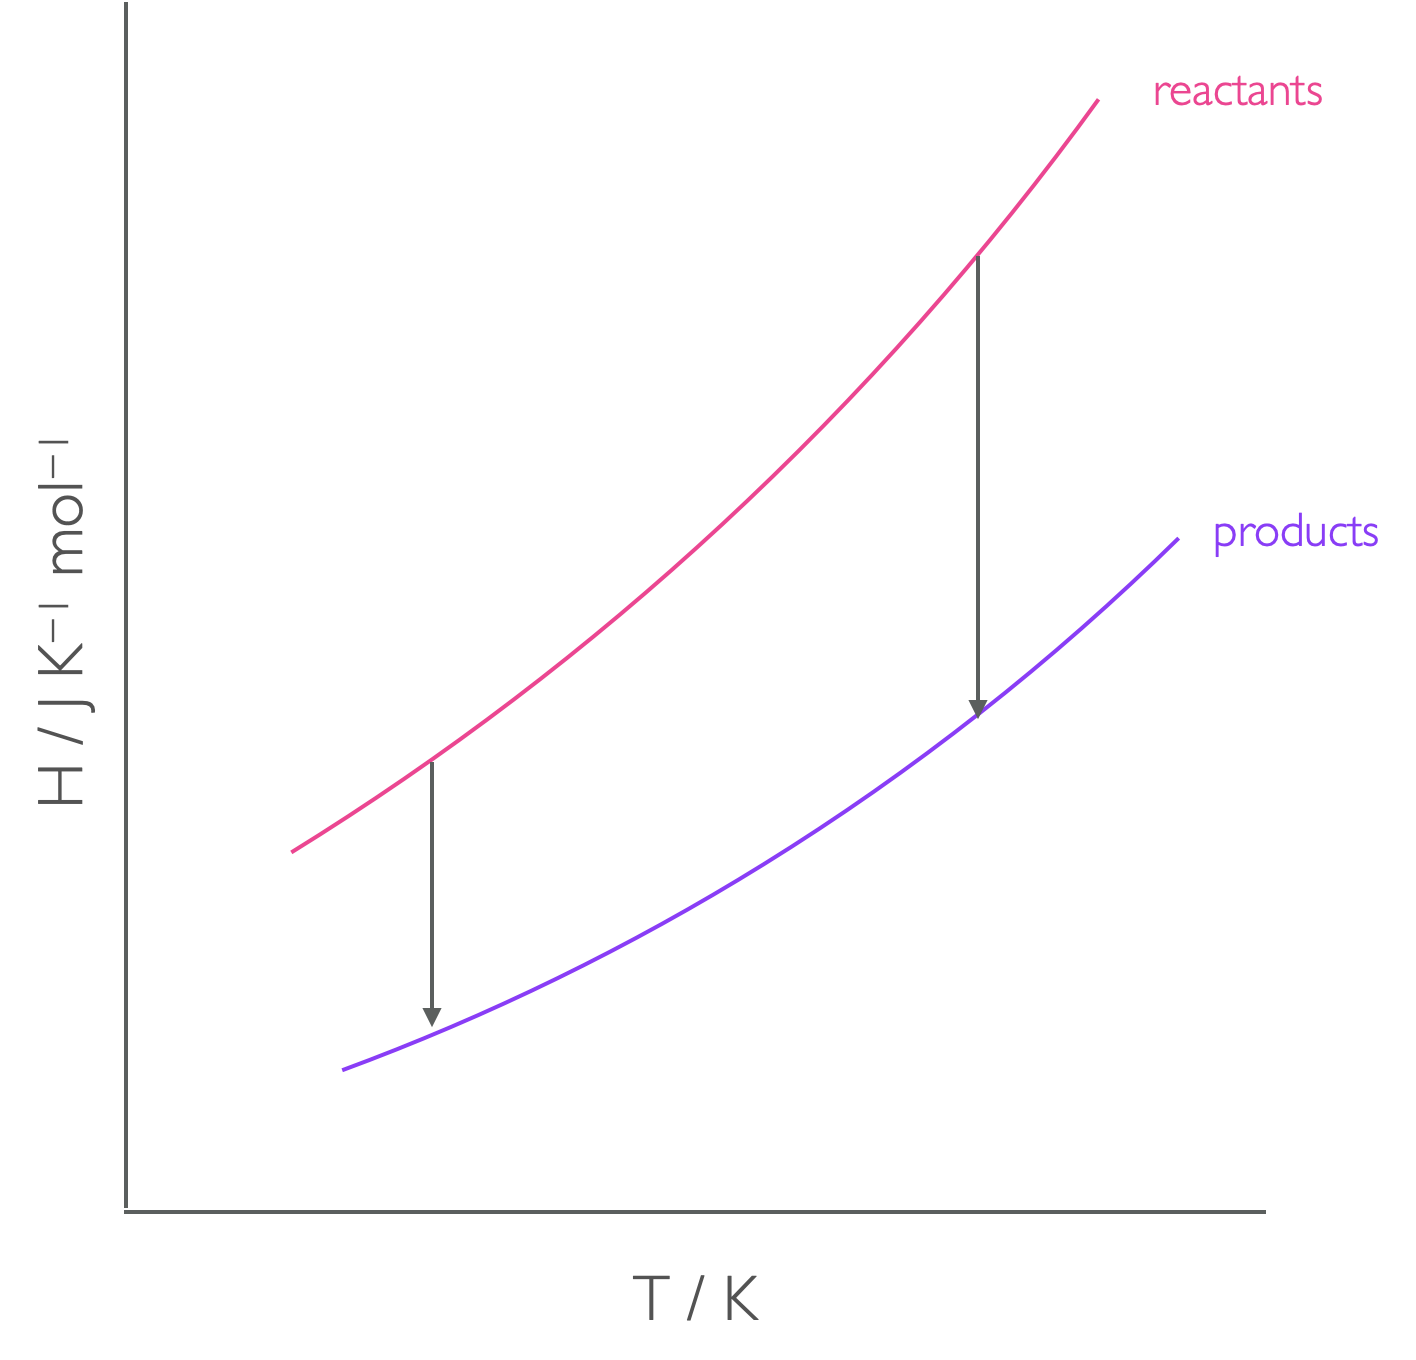
\includegraphics[width=0.7\linewidth]{images/enthalpytemp} 

}

\caption{The enthalpy of reaction is the difference in enthalpy between reactants and products, but this is tempearture dependant.}\label{fig:enthalpytemp}
\end{figure}

The value \(\Delta_r C_p^{\ominus}\) is the difference in heat capacity of the products and reactants at constant pressure. You have already seen this equation in equation \eqref{eq:heatcapacitystate} in section \ref{sec:equations1}.

For moderate changes in temperature we can assume that the heat capacity is a linear function and we can use Kirchoff's law (equation \eqref{eq:kirchoff}), but at larger temperature differences this function should really be integrated to account for the temperature dependance of heat capacity.

\hypertarget{enthalpy-of-phase-changes}{%
\section{Enthalpy of phase changes}\label{enthalpy-of-phase-changes}}

You are no doubt already familiar with the concepts of phase changes, and they are an increadibly important concept in thermodynamics which I will cover more than once during this course.

As energy in the form of heat is added to a system the temperature of that system usually increases, however there are some points where heat is added, but the temperature doesn't rise. However, at these points there is a distinct change in phase. This occurs no matter what two phases are involved.

The enthalpy of the phase change is a measure of the energy required (or released) when the intermolecular bonds between the molecules are broken or changed. Since transitions from the liquid to the gas phase involve complete breaking of the intermolecular bond enthalpies of fusion are always smaller than enthalpies of vapourisation.

\begin{figure}

{\centering 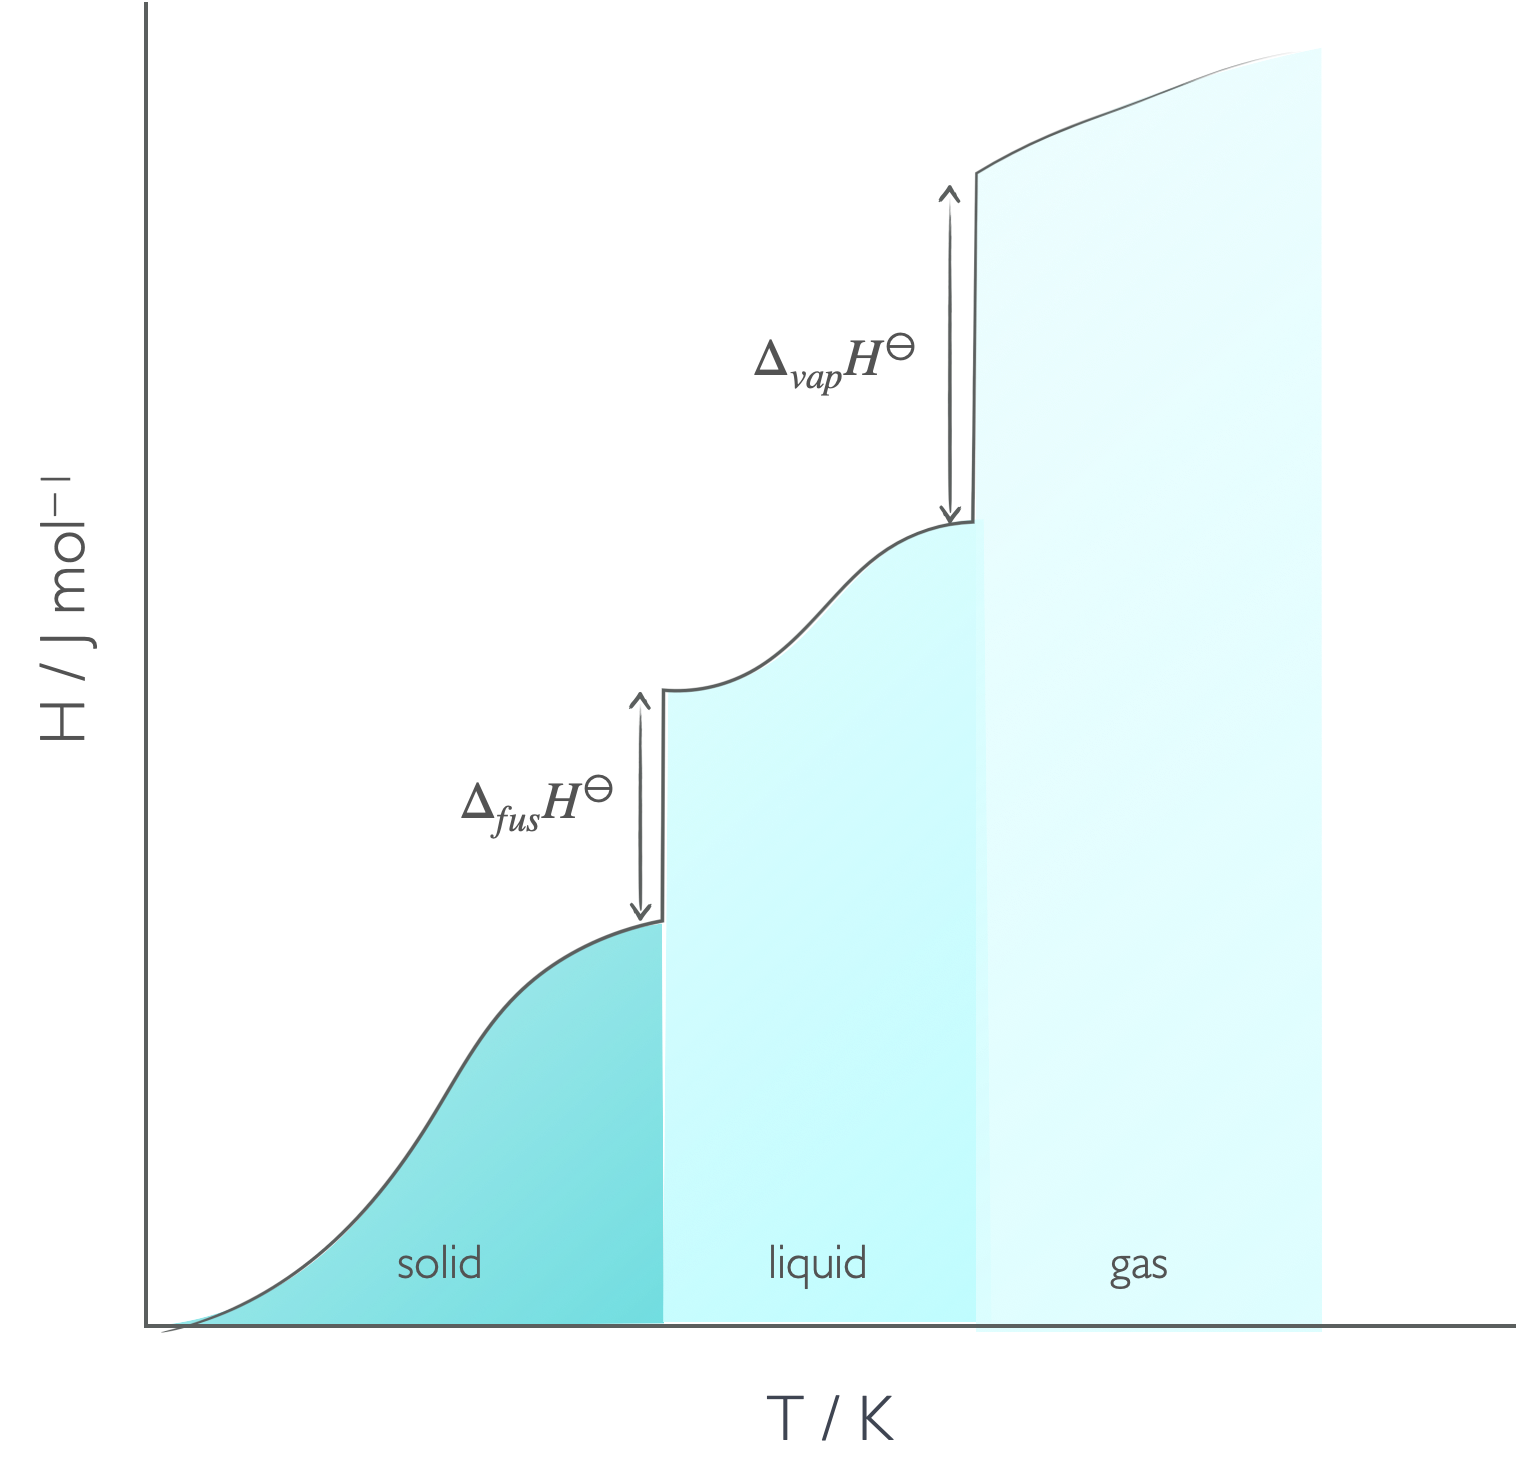
\includegraphics[width=0.7\linewidth]{images/enthalpyphasechange} 

}

\caption{As heat is added to the system usually the temperature increases, but there are points where heat is added but there is no increase in temperature, but instead a phase change.}\label{fig:enthalpyphasechange}
\end{figure}

We will meet phase changes later in the course when we consider both enthalpy and Gibbs' free energy so this is intentially just a very quick introduction.

\hypertarget{questions-2}{%
\section{Questions}\label{questions-2}}

\begin{enumerate}
\def\labelenumi{\arabic{enumi}.}
\item
  The constant pressure specific heat capacity of copper is 0.3850 kJ kg\textsuperscript{--1} K\textsuperscript{--1} at 298 K. Calculate the constant pressure heat capacity of 0.559 mol of copper at this temperature.
\item
  The constant pressure molar heat capacity of methane, CH\textsubscript{4}, is 35.31 J K\textsuperscript{--1} mol\textsuperscript{--1} at temperatures close to 298 K. Calculate the enthalpy change when 4.7 mol of methane is heated from a temperature of 266 K to 302 K.
\item
  What is the enthalpy of formation of water at 100 ºC if \(\Delta H_f = -241.82\) kJ mol\(^{-1}\) at 25 ºC? What assumptions have you made?
\end{enumerate}

c\(_{p,m} H_2 O = 33.58\) J K\(^{-1}\) mol\(^{-1}\)

c\(_{p,m} H_2 = 28.84\) J K\(^{-1}\) mol\(^{-1}\)

c\(_{p,m} O_2 = 29.37\) J K\(^{-1}\) mol\(^{-1}\)

\begin{enumerate}
\def\labelenumi{\arabic{enumi}.}
\setcounter{enumi}{3}
\tightlist
\item
  The complete combustion of ethane (C\textsubscript{2}H\textsubscript{6}) releases 1558.8 kJ mol\textsuperscript{−1} at 25 ºC. Calculate the enthalpy of combustion at 90 ºC.
\end{enumerate}

\begin{longtable}[]{@{}cc@{}}
\toprule
& C\textsubscript{p} / J K\textsuperscript{−1} mol\textsuperscript{−1}\tabularnewline
\midrule
\endhead
C\textsubscript{2}H\textsubscript{6} & 52.6\tabularnewline
O\textsubscript{2} & 29.4\tabularnewline
CO\textsubscript{2} & 37.1\tabularnewline
H\textsubscript{2}O & 75.3\tabularnewline
\bottomrule
\end{longtable}

\begin{enumerate}
\def\labelenumi{\arabic{enumi}.}
\setcounter{enumi}{4}
\tightlist
\item
  Calculate the enthalpy of formation of liquid mercury at 0 ºC. (C\textsubscript{p} = 27.98 J K\textsuperscript{−1} mol\textsuperscript{−1})
\end{enumerate}

\hypertarget{sec:w2p2ans}{%
\section{Answers}\label{sec:w2p2ans}}

\begin{enumerate}
\def\labelenumi{\arabic{enumi}.}
\tightlist
\item
  c = 13.7 J K\textsuperscript{--1}
\item
  ΔH = 6.0 kJ
\item
  \(\Delta _f H _{(\textrm{100 ºC})}=\) -242.57 kJ mol\textsuperscript{−1}
\item
  ΔH\textsubscript{363K} = -1549.4 kJ mol\textsuperscript{−1}
\item
  Δ\textsubscript{f}H\textsubscript{273K} = 0 kJ mol\textsuperscript{−1}
\end{enumerate}

\hypertarget{ch:Part5}{%
\chapter{Week 3 - Part 1}\label{ch:Part5}}

\hypertarget{one-last-thing-before-we-introduce-entropy}{%
\section{One last thing before we introduce entropy}\label{one-last-thing-before-we-introduce-entropy}}

\emph{The following video has been added for some context to the material, it is not core to the course and the material in it is not examinable.}

Thermodynamics was developed to understand steam engines better, to help improve their design.

It was found that no matter how well designed the boiler or pistons the efficiency of a steam engine was controlled by something engineers have no control over - them temperature of the surroundings.

\begin{equation}
\epsilon = 1-\frac{T_{\textrm{sink}}}{T_{\textrm{source}}}
\label{eq:efficiency}
\end{equation}

It was these experiments on efficiency by William Thompson (later Lord Kelvin) which lead to the concept of thermodynamic temperature we have already met in section \ref{sec:zeroth}.

This equation for efficiency (equation \eqref{eq:efficiency}) says that a thermodynamic system (or steam engine) can only ever be 100\% efficient if either the temperature of the `sink' (or the surroundings as we have come to call them) is absolute zero, or else the temperature of the source (or system) is infinite. Clearly neither of these cases can ever be true and so no system will ever be, can ever be, 100\% efficient.

The reason you can never have 100\% efficiency is entropy\ldots{} but what is entropy?

\hypertarget{thermodynamic-spontaneity}{%
\section{Thermodynamic spontaneity}\label{thermodynamic-spontaneity}}

In thermodynamics when a process is spontaneous it will occur without work needing to be done to bring about any change.

This phrase can be turned around to say that work can be done to make a non-spontaneous process to occur.

\begin{figure}

{\centering 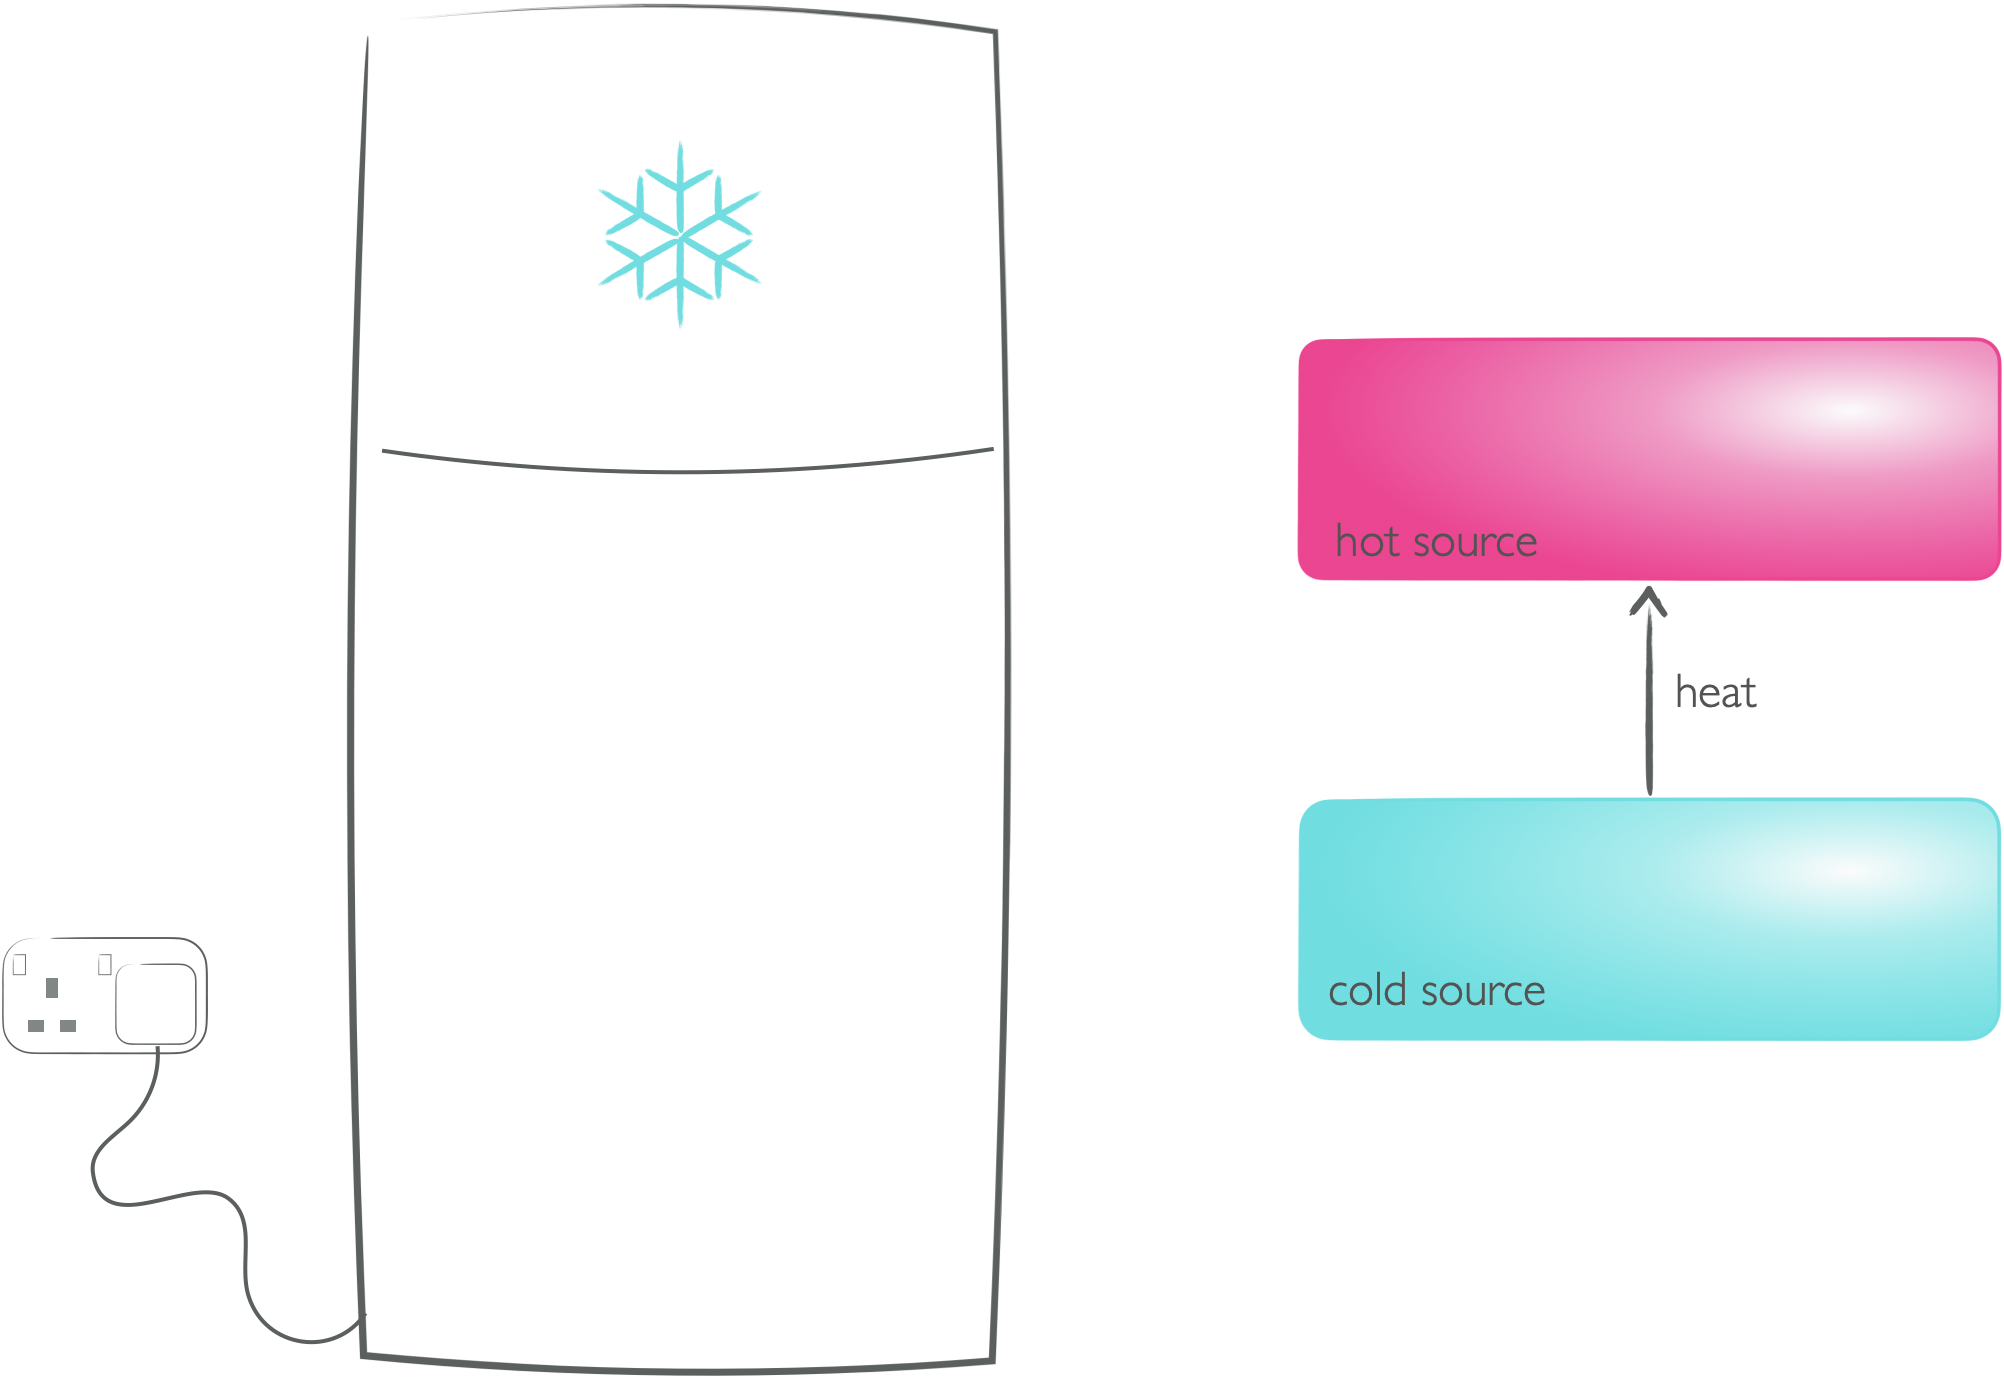
\includegraphics[width=0.5\linewidth]{images/fridge} 

}

\caption{Fridges and freezers show that non-sponteneous processes can occur if work is done to make them happen - heat does not spontaneously from from cold bodies to hot bodies, but doing work (with the pump in the fridge) allows this thermodynamically non-spontenous process to occur.}\label{fig:fridge}
\end{figure}

It is important to not confuse spontaneous processes with kinetics, a process may be spontaneous but occur very slowly. Spontaneity is just about the thermodynamics.

If a balloon contains a mixture of hydrogen gas and oxygen gas it will happily just float there not reacting at room temperature - it is only when a spark is added to the system that the gases react to form water. Without a spark the kinetics are very, very slow, but the reaction is still spontaneous.

\emph{There will be more about this process later in the course, as some people confuse the reaction of gases to form a liquid as being non-spontaneous.}

\hypertarget{sec:2ndlaw}{%
\section{Second Law of Thermodyanamics}\label{sec:2ndlaw}}

Just like the first law there are various statements of the first law of thermodynamics, because various people were working on the same problem at the same time.

The most famous of these statements is:

`the entropy of an isolated system tends to increase'

and another common statement which considers systems which are not isolated:

`the entropy of a universe increases during any spontaneous change'

Clausius linked the change in entropy of a system to the `heat' added to that system reversibly, where temperature is again a factor:

\begin{equation}
\Delta S=\frac{q_{\textrm{rev}}}{T}
\label{eq:clausius}
\end{equation}

This equation says that the entropy increase for a given amount of heat is greater at lower temperatures. This is the minimum amount of entropy change (if the process isn't reversible then the entropy change is higher).

This is often stated as the clausius inequality (where the heat isn't considered to be exchanged reversibly):

\begin{equation}
\Delta S \geq \frac {q}{T}
\label{eq:clausiusineq}
\end{equation}

One thing entropy is \textbf{not} is dis*****! This is not an acceptable understanding of entropy - please try and forget the `d-word' when thinking about entropy.

\hypertarget{the-statistical-nature-of-entropy}{%
\section{The statistical nature of entropy}\label{the-statistical-nature-of-entropy}}

If we look at two bulbs, one containing gas and the other vacuumm and open the tap between the two containers we are not surprised when the gas distributes between the two bulbs.

\begin{figure}

{\centering 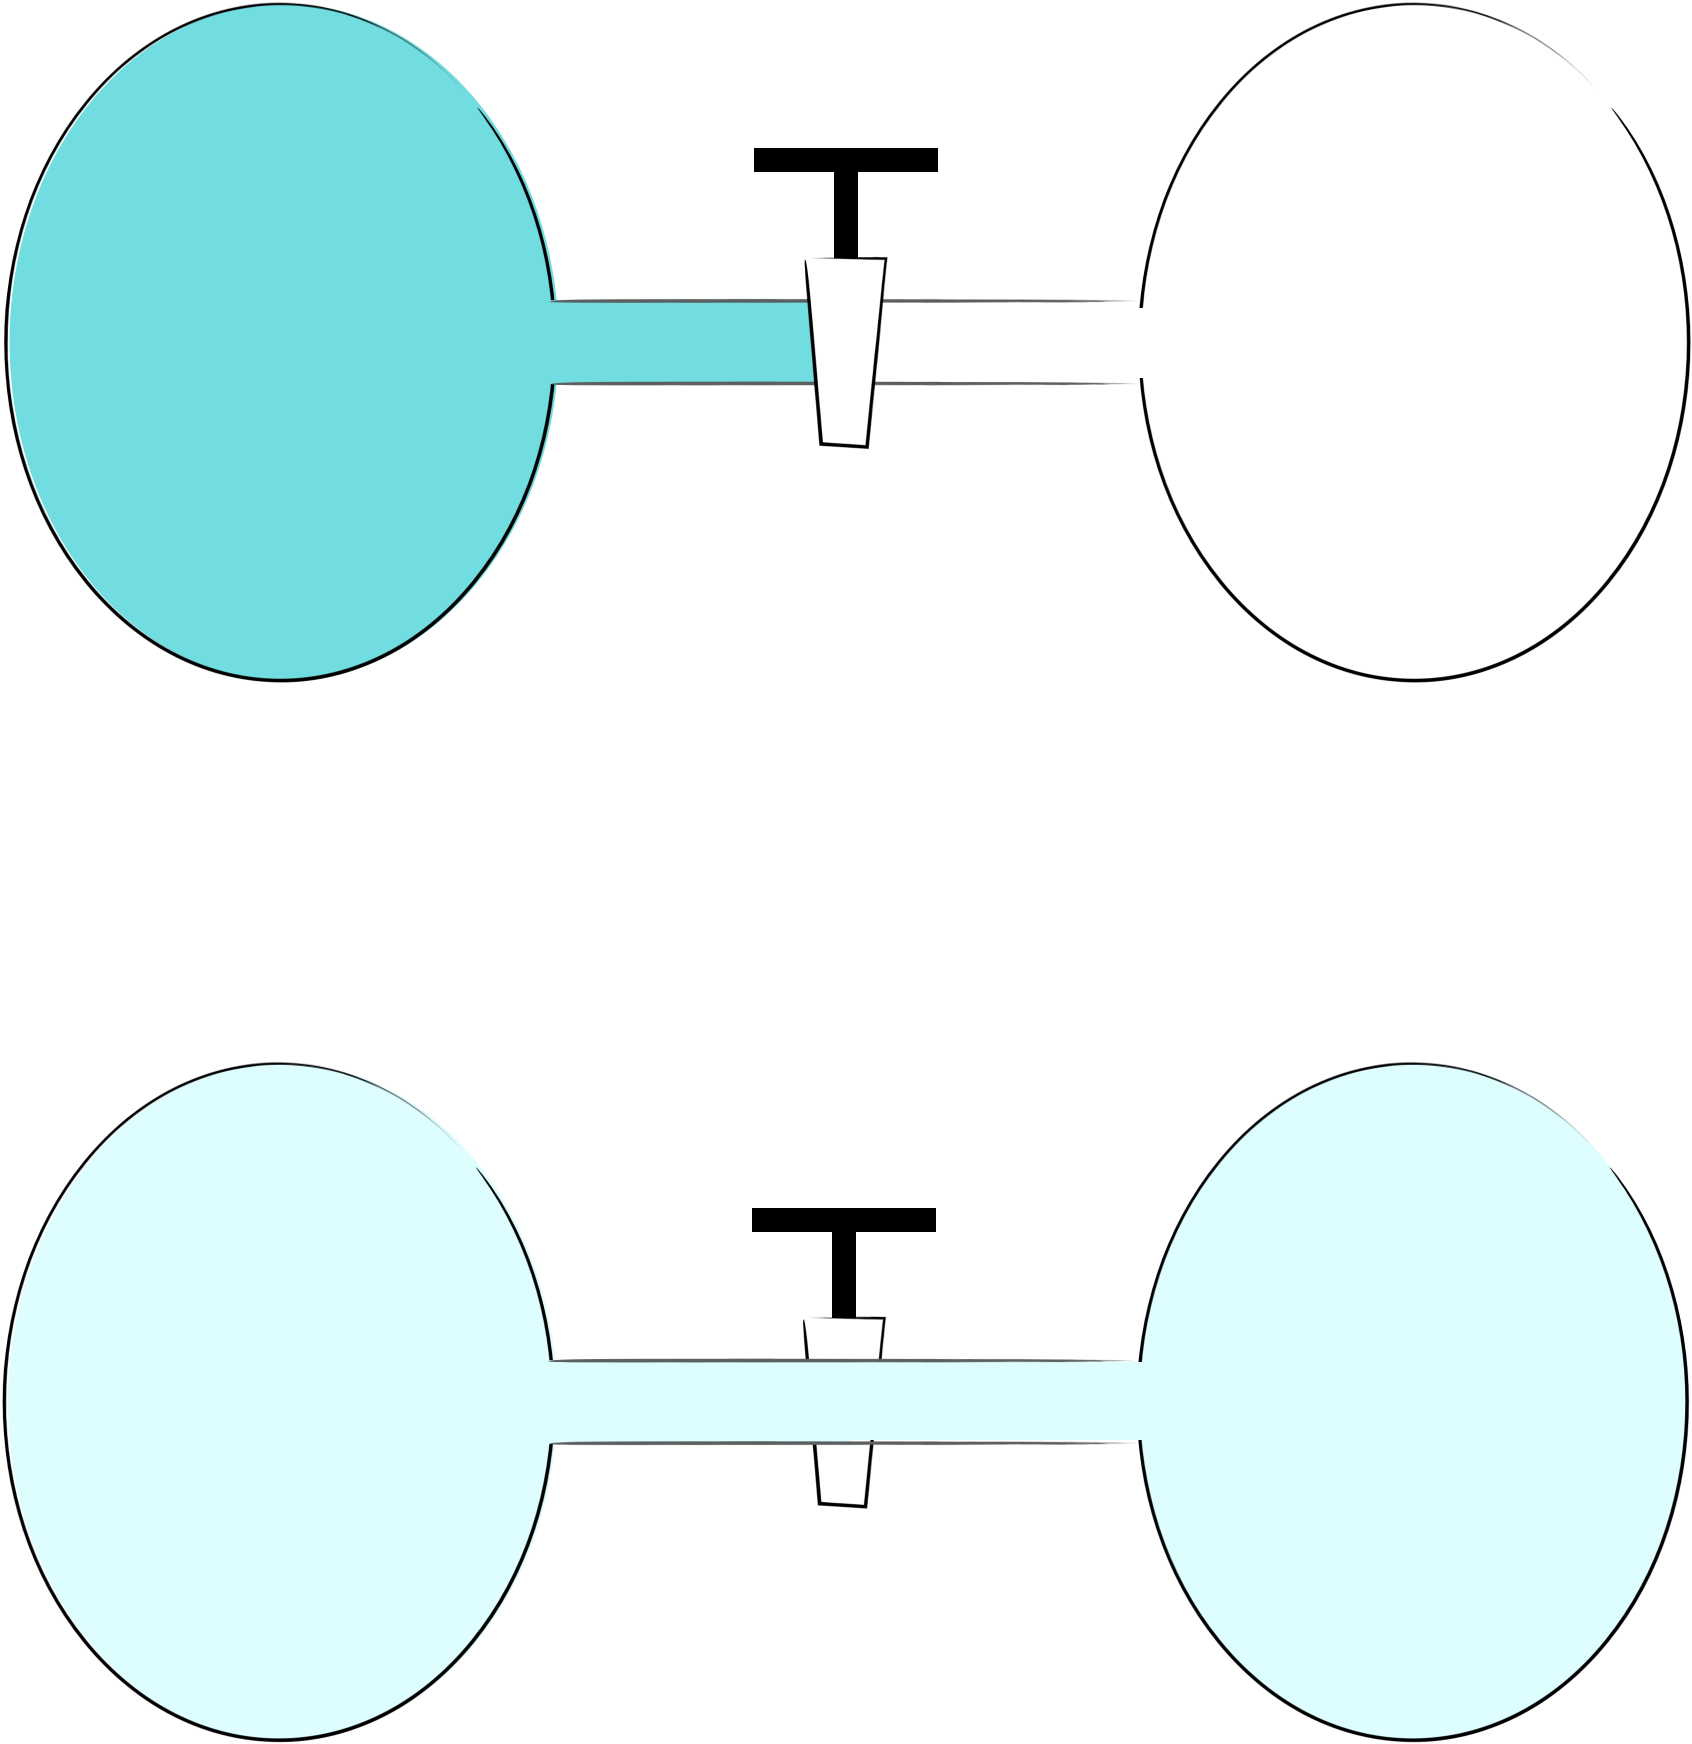
\includegraphics[width=0.5\linewidth]{images/gasdistribution} 

}

\caption{If we have two bulbs, one with gas the other with vacuum and open the tap it is unsurprising that the gas distributes evenly between the two bulbs.}\label{fig:gasdistribution}
\end{figure}

\hypertarget{macrostates}{%
\subsection{Macrostates}\label{macrostates}}

So what is happening on a molecular level? Simplifying the system to just 4 particles in the two bulbs, there are 5 possible ways of arranging this system (figure \ref{fig:macro}).

\begin{figure}

{\centering 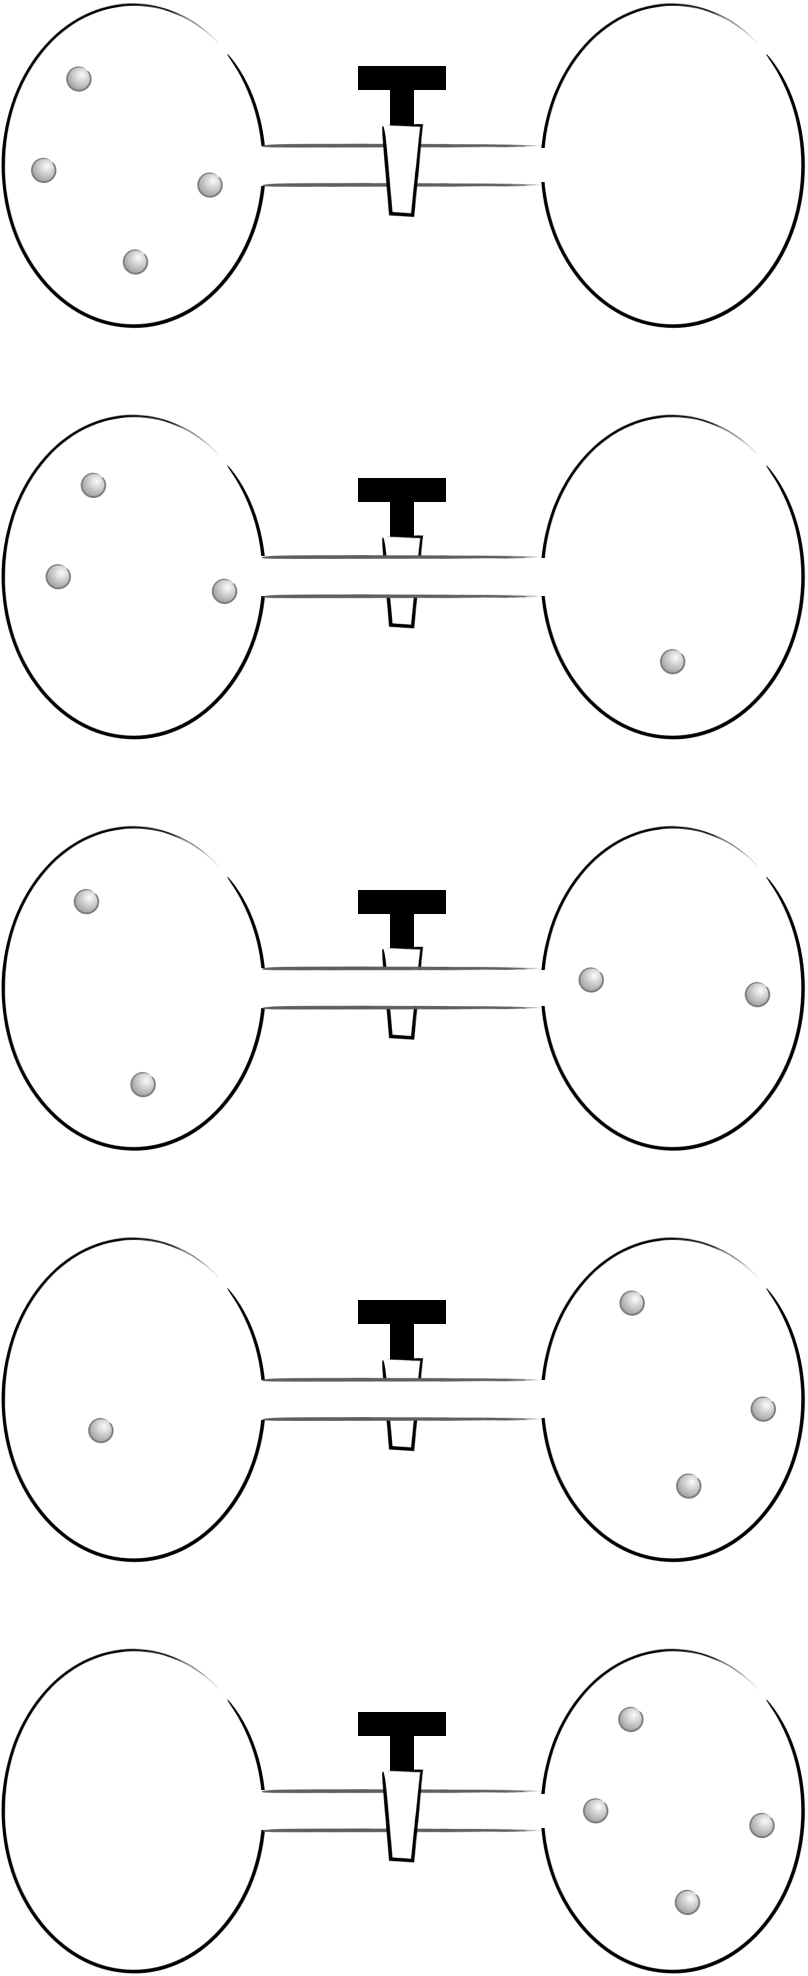
\includegraphics[width=0.5\linewidth]{images/macro} 

}

\caption{There are five possible ways of aranging four particles between two bulbs.}\label{fig:macro}
\end{figure}

Each of these possible arrangements are called the macrostates of the system, however the probability of achieving each of these macrostates is not the same.

\hypertarget{microstates}{%
\subsection{Microstates}\label{microstates}}

The probability of any one of these states occuring depends upon the number of microstates making up each macrostate. If we consider this system and imagine we can individually name each atom:

\begin{itemize}
\tightlist
\item
  all `atoms' in the LH container there is only one possible arrangement
\item
  all `atoms' in the RH container there is only one possible arrangement
\item
  3 `atoms' in the LH container and 1 in the RH there are four possible arrangements
\item
  3 `atoms' in the RH container and 1 in the LH there are four possible arrangements
\item
  2 `atoms' in the LH container and 2 in the RH container there are six possible arrangements
\end{itemize}

The total number of permutations is 2\textsuperscript{4} = 16.

The total number of permutations of any system is given by:

\begin{equation}
\textrm{permutation}=\textrm{possible outcomes}^\textrm{number of particles}
\label{eq:permutations}
\end{equation}

and the multiplicity of microstates is given by:

\begin{equation}
\Omega = \frac{N!}{n_A!n_B!}
\label{eq:multiplicity}
\end{equation}

The probability of any given state occuring is the number of microstates making up a macrostate divided by the total number of permutations of the system.

\begin{figure}

{\centering 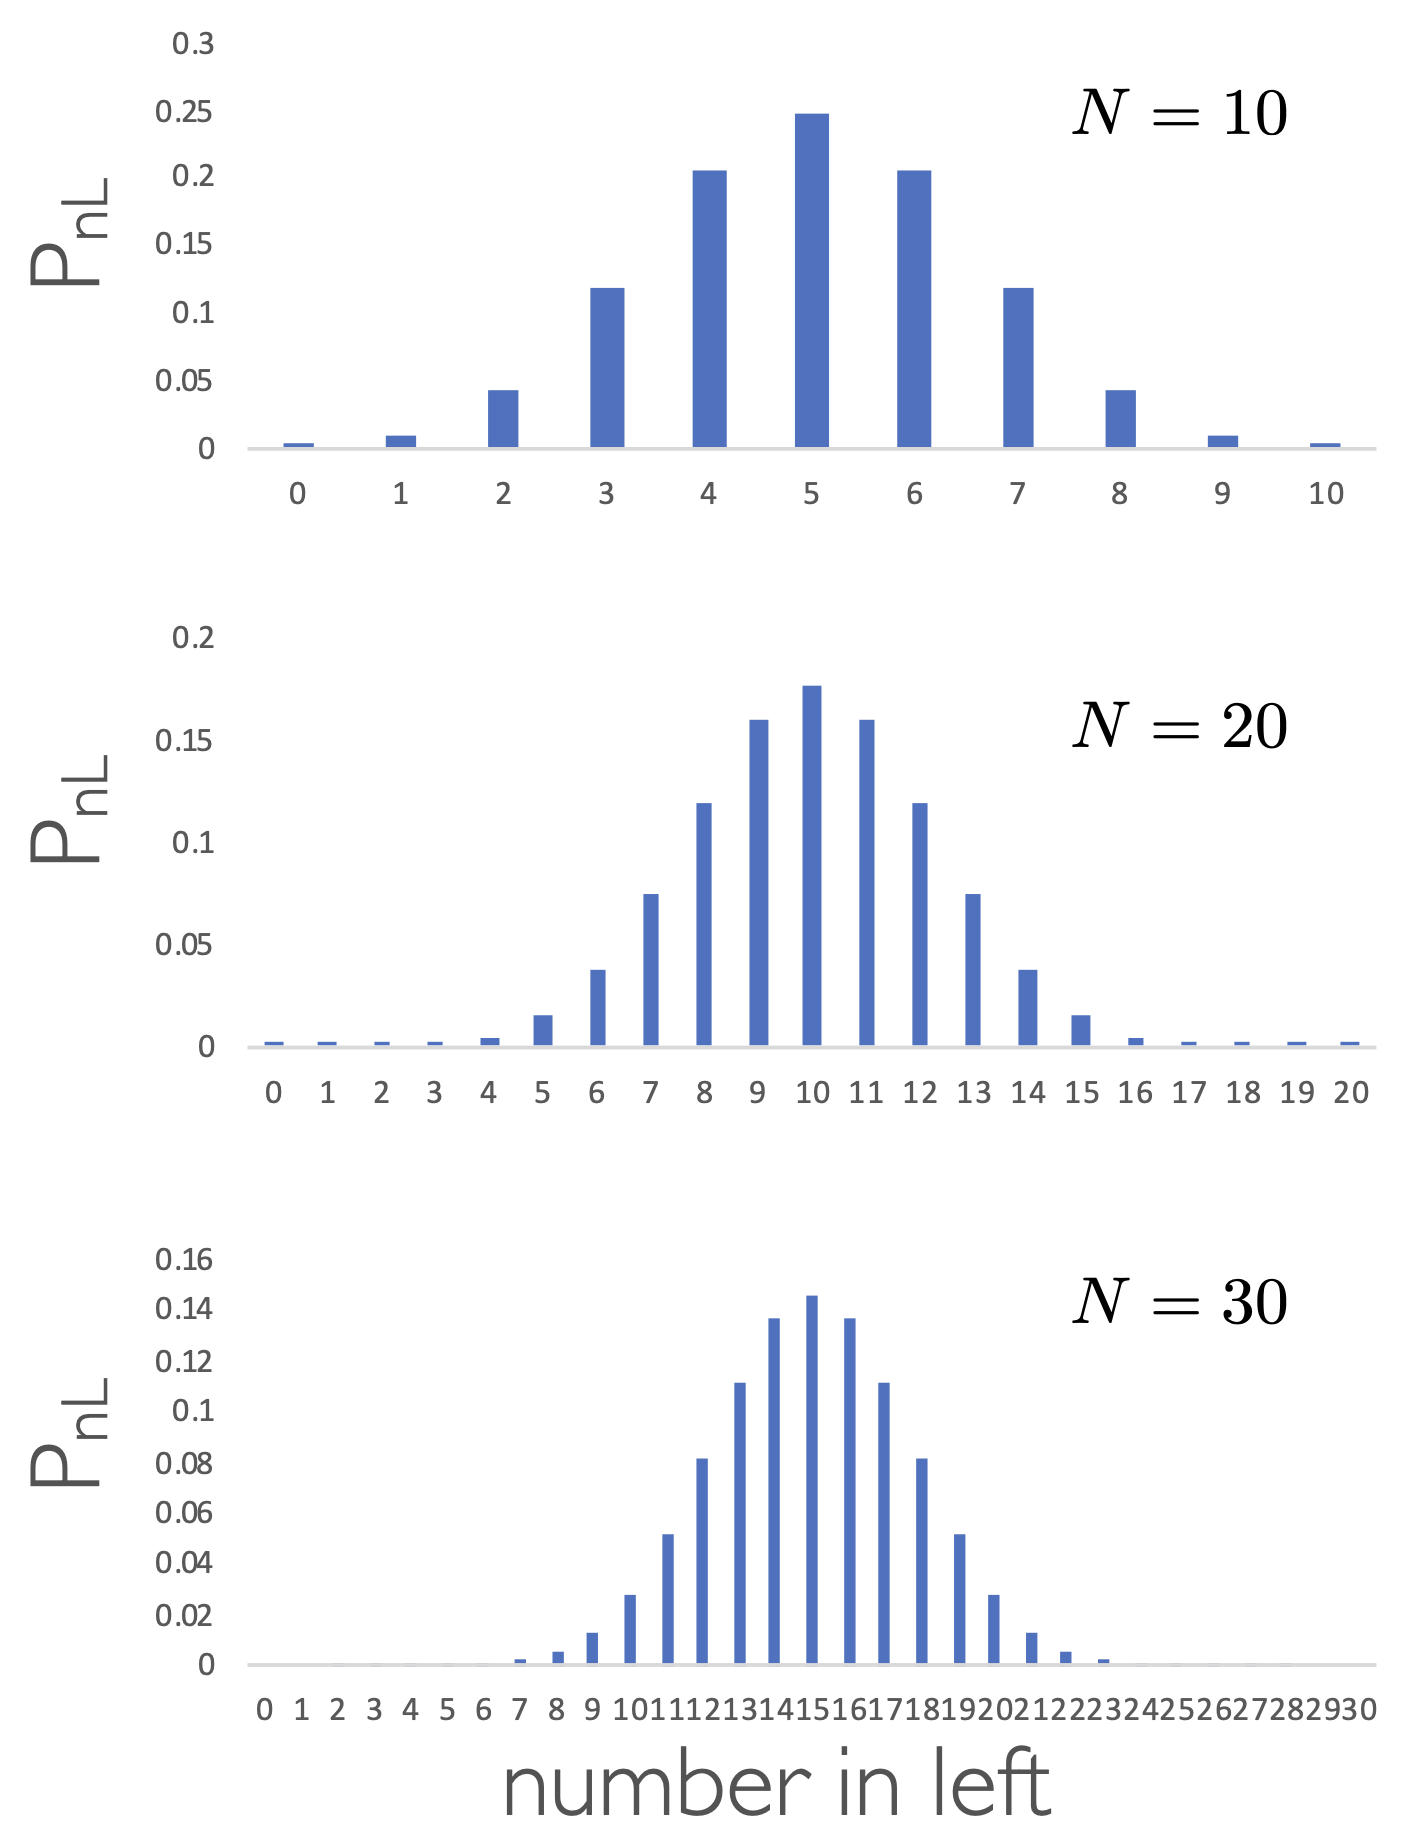
\includegraphics[width=0.5\linewidth]{images/probabilityleft} 

}

\caption{The probability of the number of particles in the left hand container for systems containing 10 (top), 20 (middle) and 30 (bottom) particles.}\label{fig:probabilityleft}
\end{figure}

\hypertarget{statistical-entropy}{%
\subsection{Statistical entropy}\label{statistical-entropy}}

Logic says that entropy is an extensive property, if we have twice as much stuff we have twice the entropy. However system permutations are not additive.

Boltzman related the permutations of a system to the absolute entropy of the system (equation \eqref{eq:boltzmann}.

\begin{equation}
S=\textrm{k}_B \ln \Omega
\label{eq:boltzmann}
\end{equation}

Boltzmann was actually concerned with the distribution of energy in a system. If you recall the total internal energy (our macrostate) is the sum of the particles each having different energies (our microstates), we said that the probability of existing in a given energy level (or microstate) fell exponentially.

Therefore as the temperature falls the probability of being in any given microstate increases and the entropy of the system decreases.

\begin{figure}

{\centering 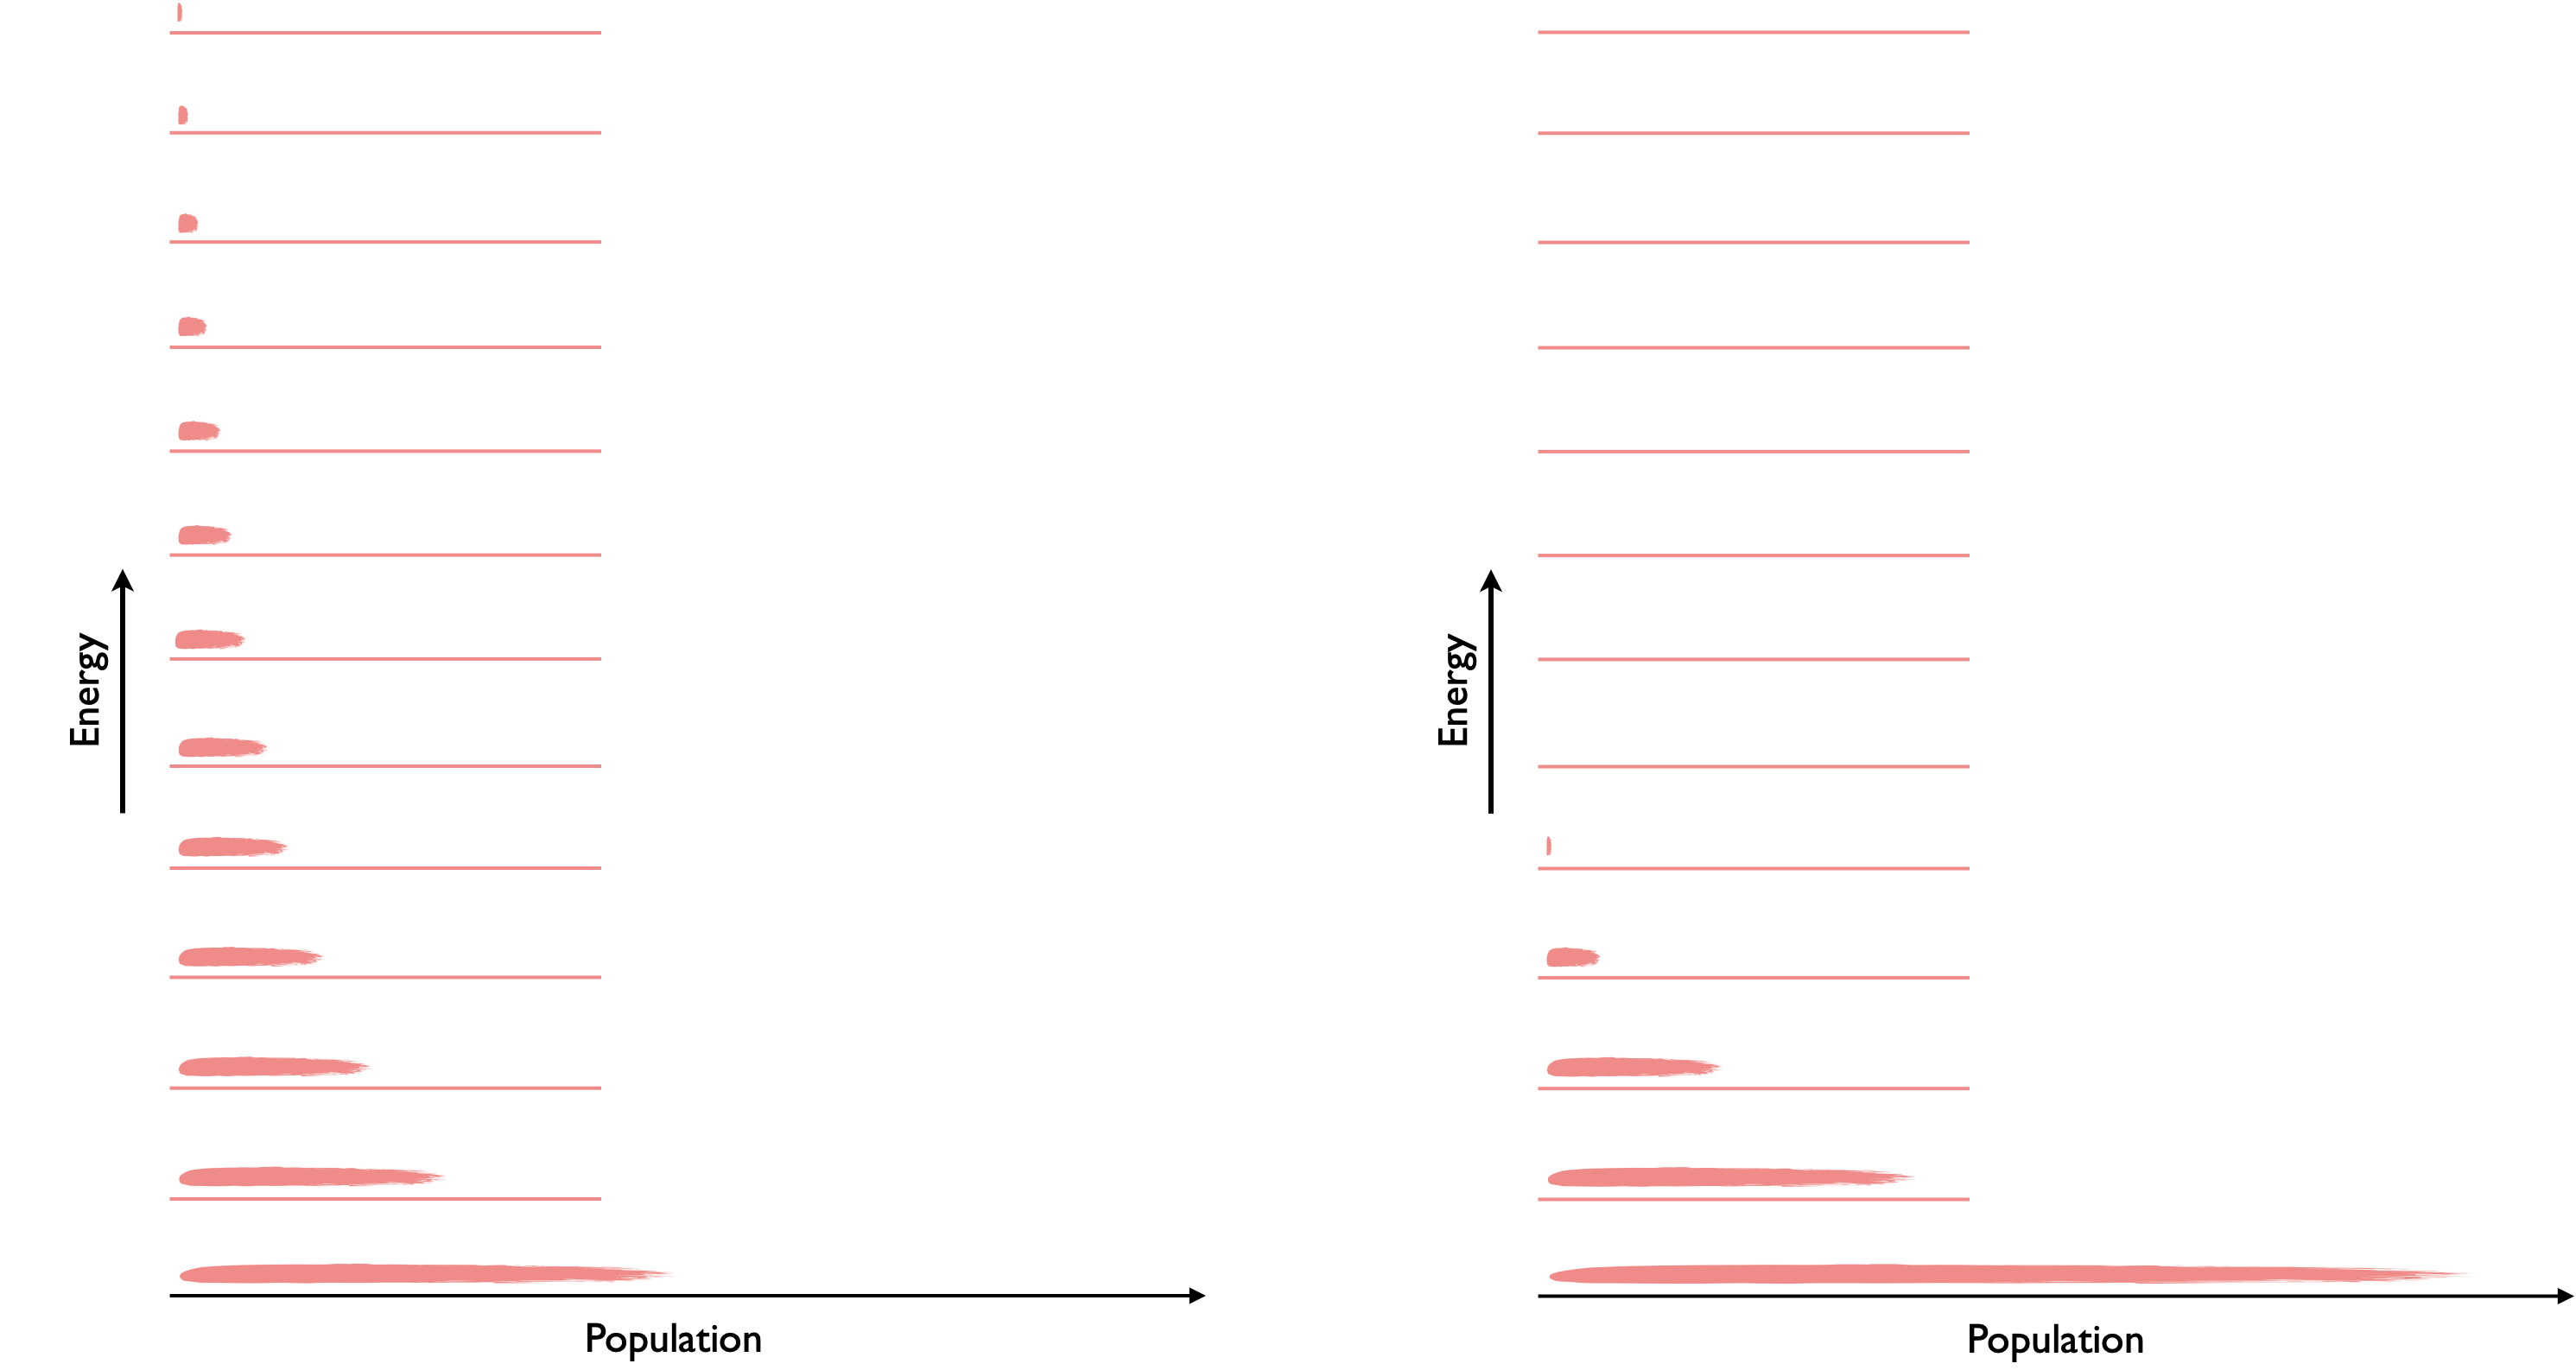
\includegraphics[width=0.8\linewidth]{images/tempentropy} 

}

\caption{As the temperature of the system falls the probability of being in a particular level increases and so the temperature falls.}\label{fig:tempentropy}
\end{figure}

\hypertarget{sec:w3p1question}{%
\section{Questions}\label{sec:w3p1question}}

\begin{enumerate}
\def\labelenumi{\arabic{enumi}.}
\item
  What is the change in entropy of a system is 50.0 kJ of energy is reversibly added in the form of heat to 100 g of water at exactly 10 ºC?
\item
  Consider a system with two bulbs and 20 particles. What is the probability that all 20 atoms will be found in a single bulb?
\item
  When 1 mol of trichloromethane is heated from 5°C to 20°C at constant pressure, the
  change of entropy is + 6.00 J K\textsuperscript{−1} mol\textsuperscript{−1} . When the solvent is heated further from 20 °C to 35°C, the change in entropy will also be + 6.00 J K\textsuperscript{−1} mol\textsuperscript{−1}. State whether this is true and justify your reasoning. You may assume C\textsubscript{p} is constant over this range.
\end{enumerate}

\hypertarget{sec:w3p1ans}{%
\section{Answers}\label{sec:w3p1ans}}

\begin{enumerate}
\def\labelenumi{\arabic{enumi}.}
\item
  ΔS = +177 J K\textsuperscript{−1}
\item
  \(\frac{2}{2^{20}}\)
\item
  No.~Entropy changes for the same input of heat are greater at lower tempeartures.
\end{enumerate}

\hypertarget{ch:Part6}{%
\chapter{Week 3 - Part 2}\label{ch:Part6}}

\hypertarget{how-temperature-affects-entropy}{%
\section{How temperature affects entropy}\label{how-temperature-affects-entropy}}

The absolute entropy of a substance is the area underneath the plot of \(\frac{C_p}{T}\) against \(T\) between absolute zero and the temperature of interest. As shown in figure \ref{fig:entropytemp} the entropy difference going between the two temperatures is teh area underneath the curve between the initial and final temperatures.

\begin{figure}

{\centering 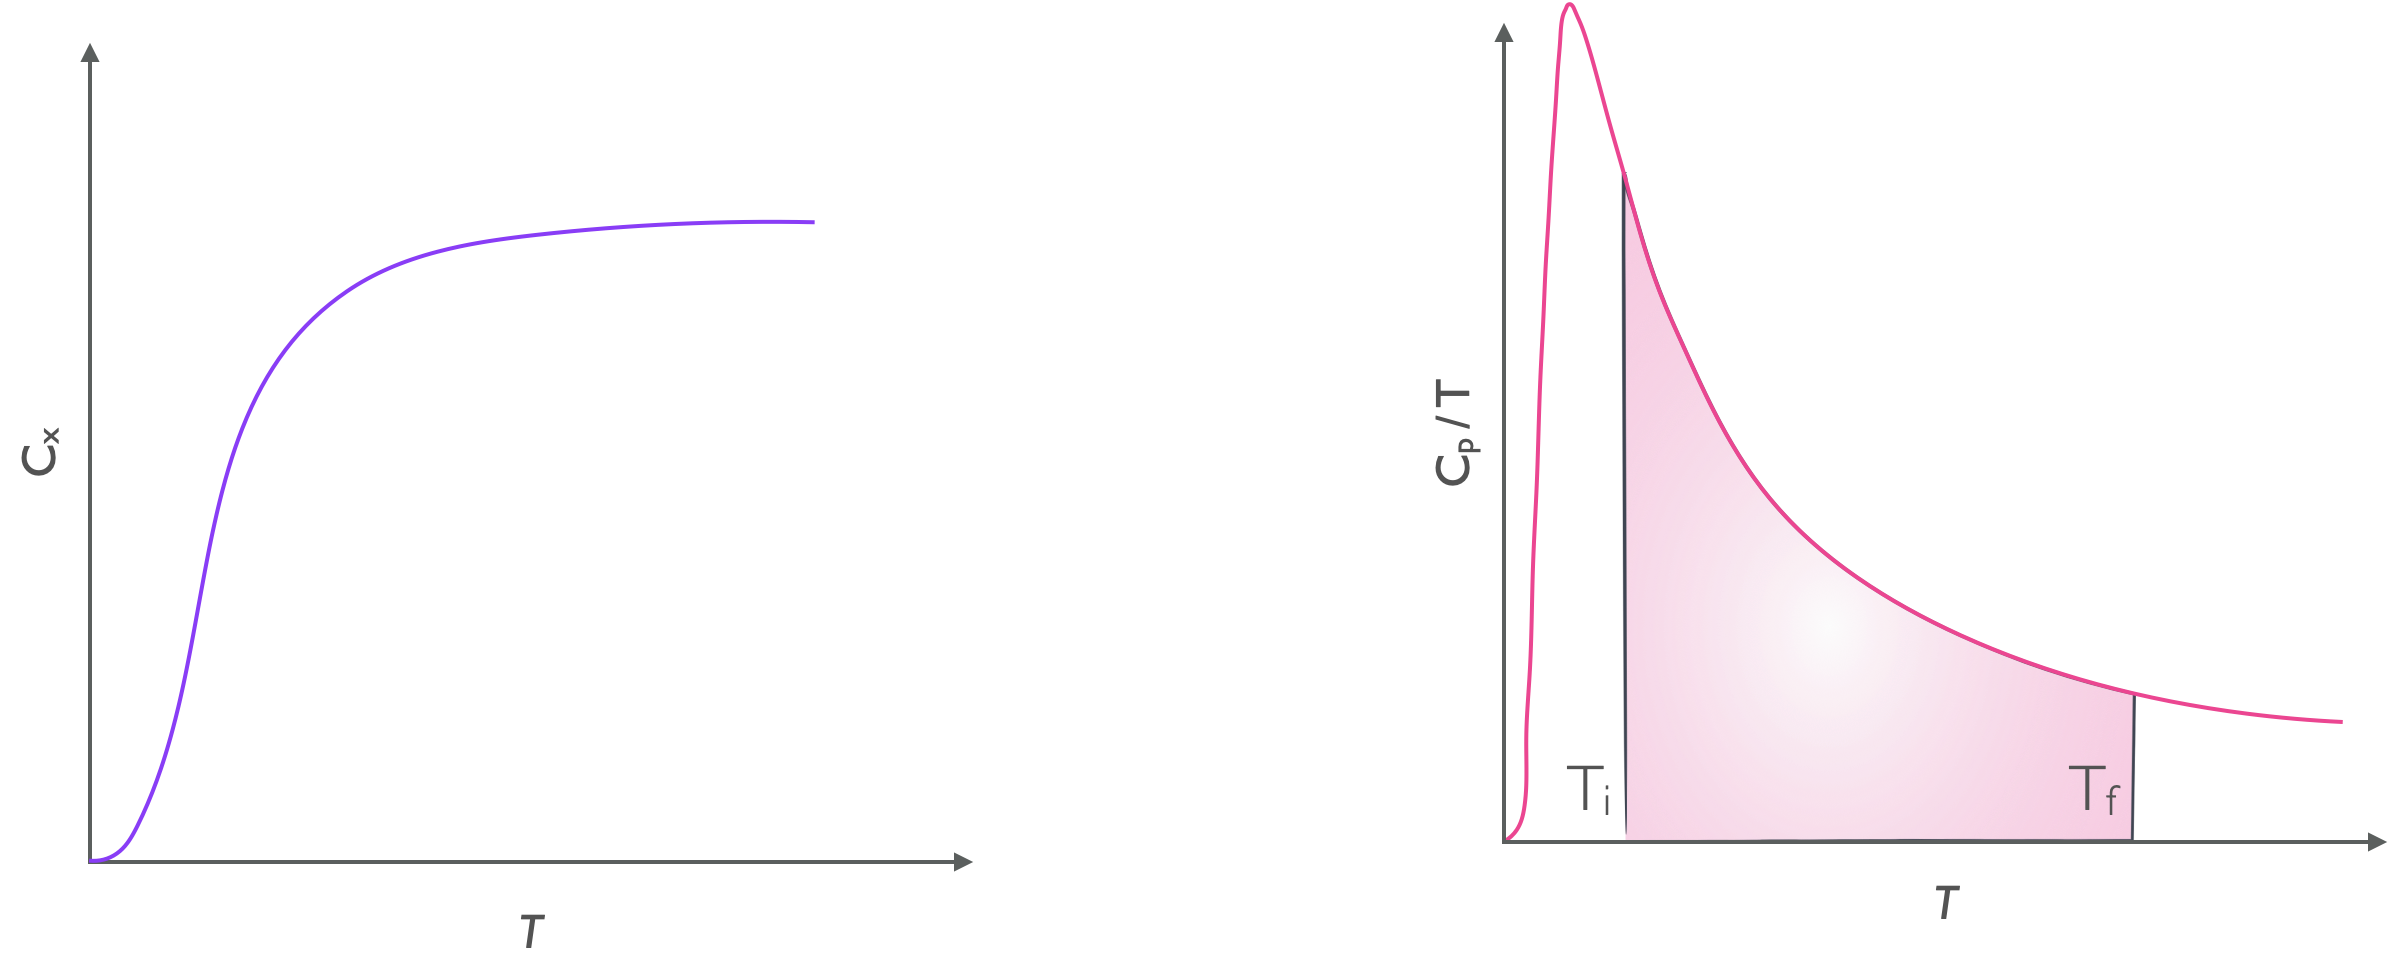
\includegraphics[width=0.8\linewidth]{images/entropytemp} 

}

\caption{The entropy change of a substance is the area of the left hand plot between teh initial and final temperature.}\label{fig:entropytemp}
\end{figure}

From equation \eqref{eq:clausius} the entropy change of heating or cooling a substance is given by:

\begin{equation}
\Delta S=C_x \ln \frac{T_f}{T_i}
\label{eq:entropytemp}
\end{equation}

and the bigger the value of heat capacity (\(C_x\)) the bigger the change in entropy for the same change in temperature.

\begin{figure}

{\centering 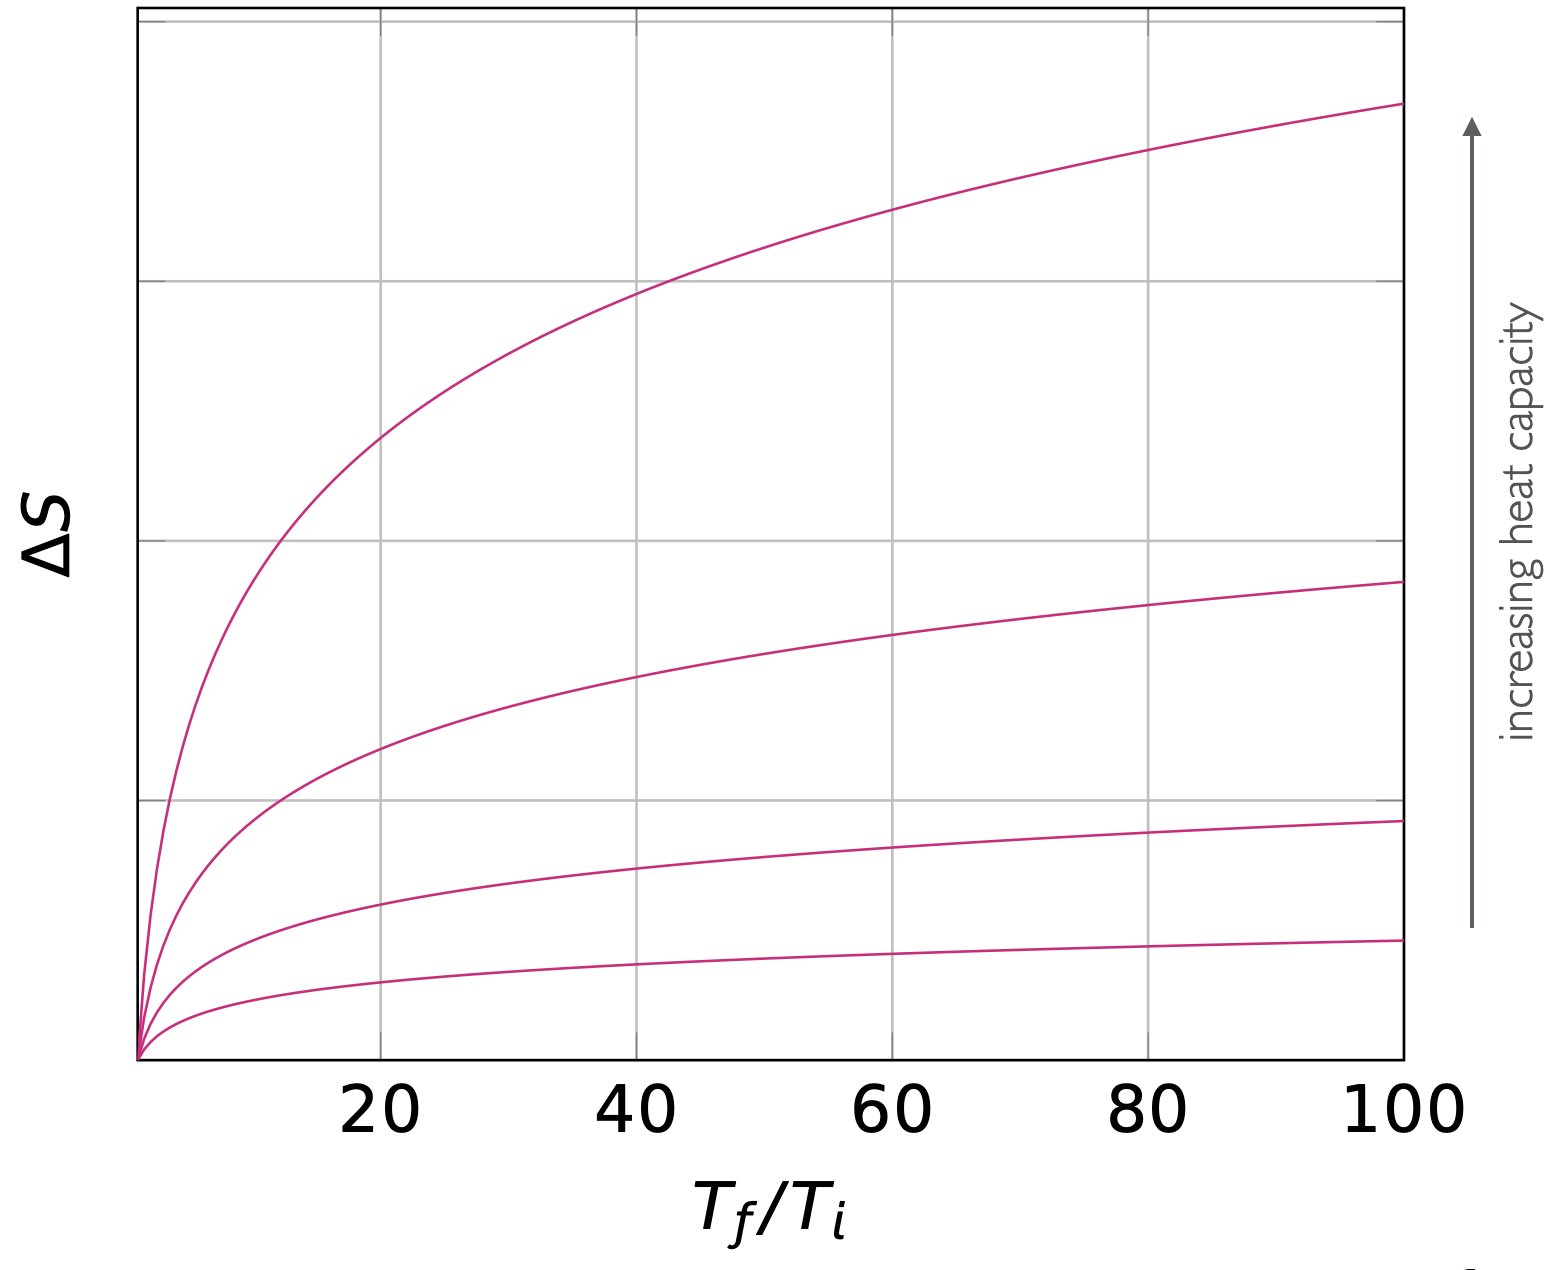
\includegraphics[width=0.8\linewidth]{images/entropyheatcapacity} 

}

\caption{The entropy change going between two temperatures is larger for substances with larger heat capacities.}\label{fig:entropyheatcapacity}
\end{figure}

For any chemical process we can now work out the entropy change for the reaction at a new temperature, assuming the heat capacity is constant over the temperature range considered.

\begin{equation}
\Delta S_{T_f} = \Delta S_{T_i} + C_x \ln \frac{T_f}{T_i}
\label{eq:entropyrxntemp}
\end{equation}

\hypertarget{the-entropy-of-phase-changes}{%
\section{The entropy of phase changes}\label{the-entropy-of-phase-changes}}

If we look at how the heat capacity divided by temperature changes as a function of temperature we see clear breaks in function where the phase changes are (figure \ref{fig:Cpphase}).

\begin{figure}

{\centering 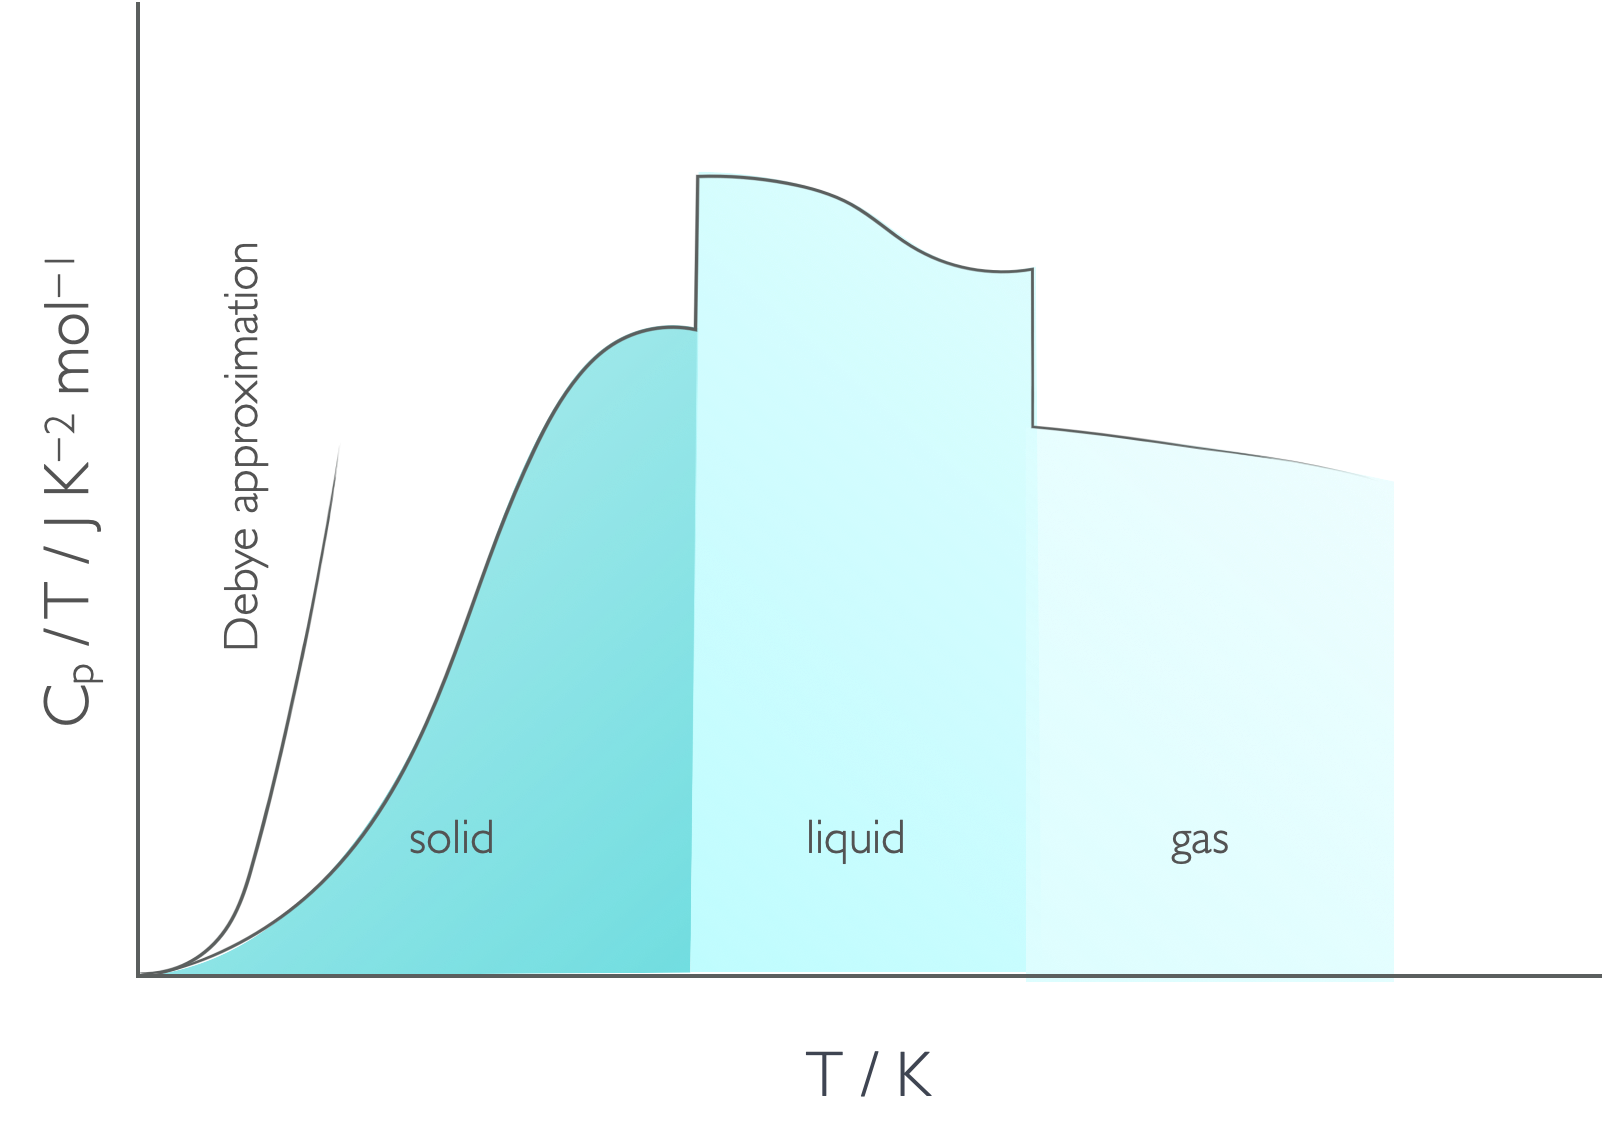
\includegraphics[width=0.8\linewidth]{images/Cpphase} 

}

\caption{The phase changes are obvious on a plot of Cp/T against T showing the latent heat of the phase change clearly. Recall that the absolute entropy of a substanced is the area under this plot.}\label{fig:Cpphase}
\end{figure}

The absolute molar entropy of a substance is sum of the entropy for heating and the entropy of the phase change.

\begin{figure}

{\centering 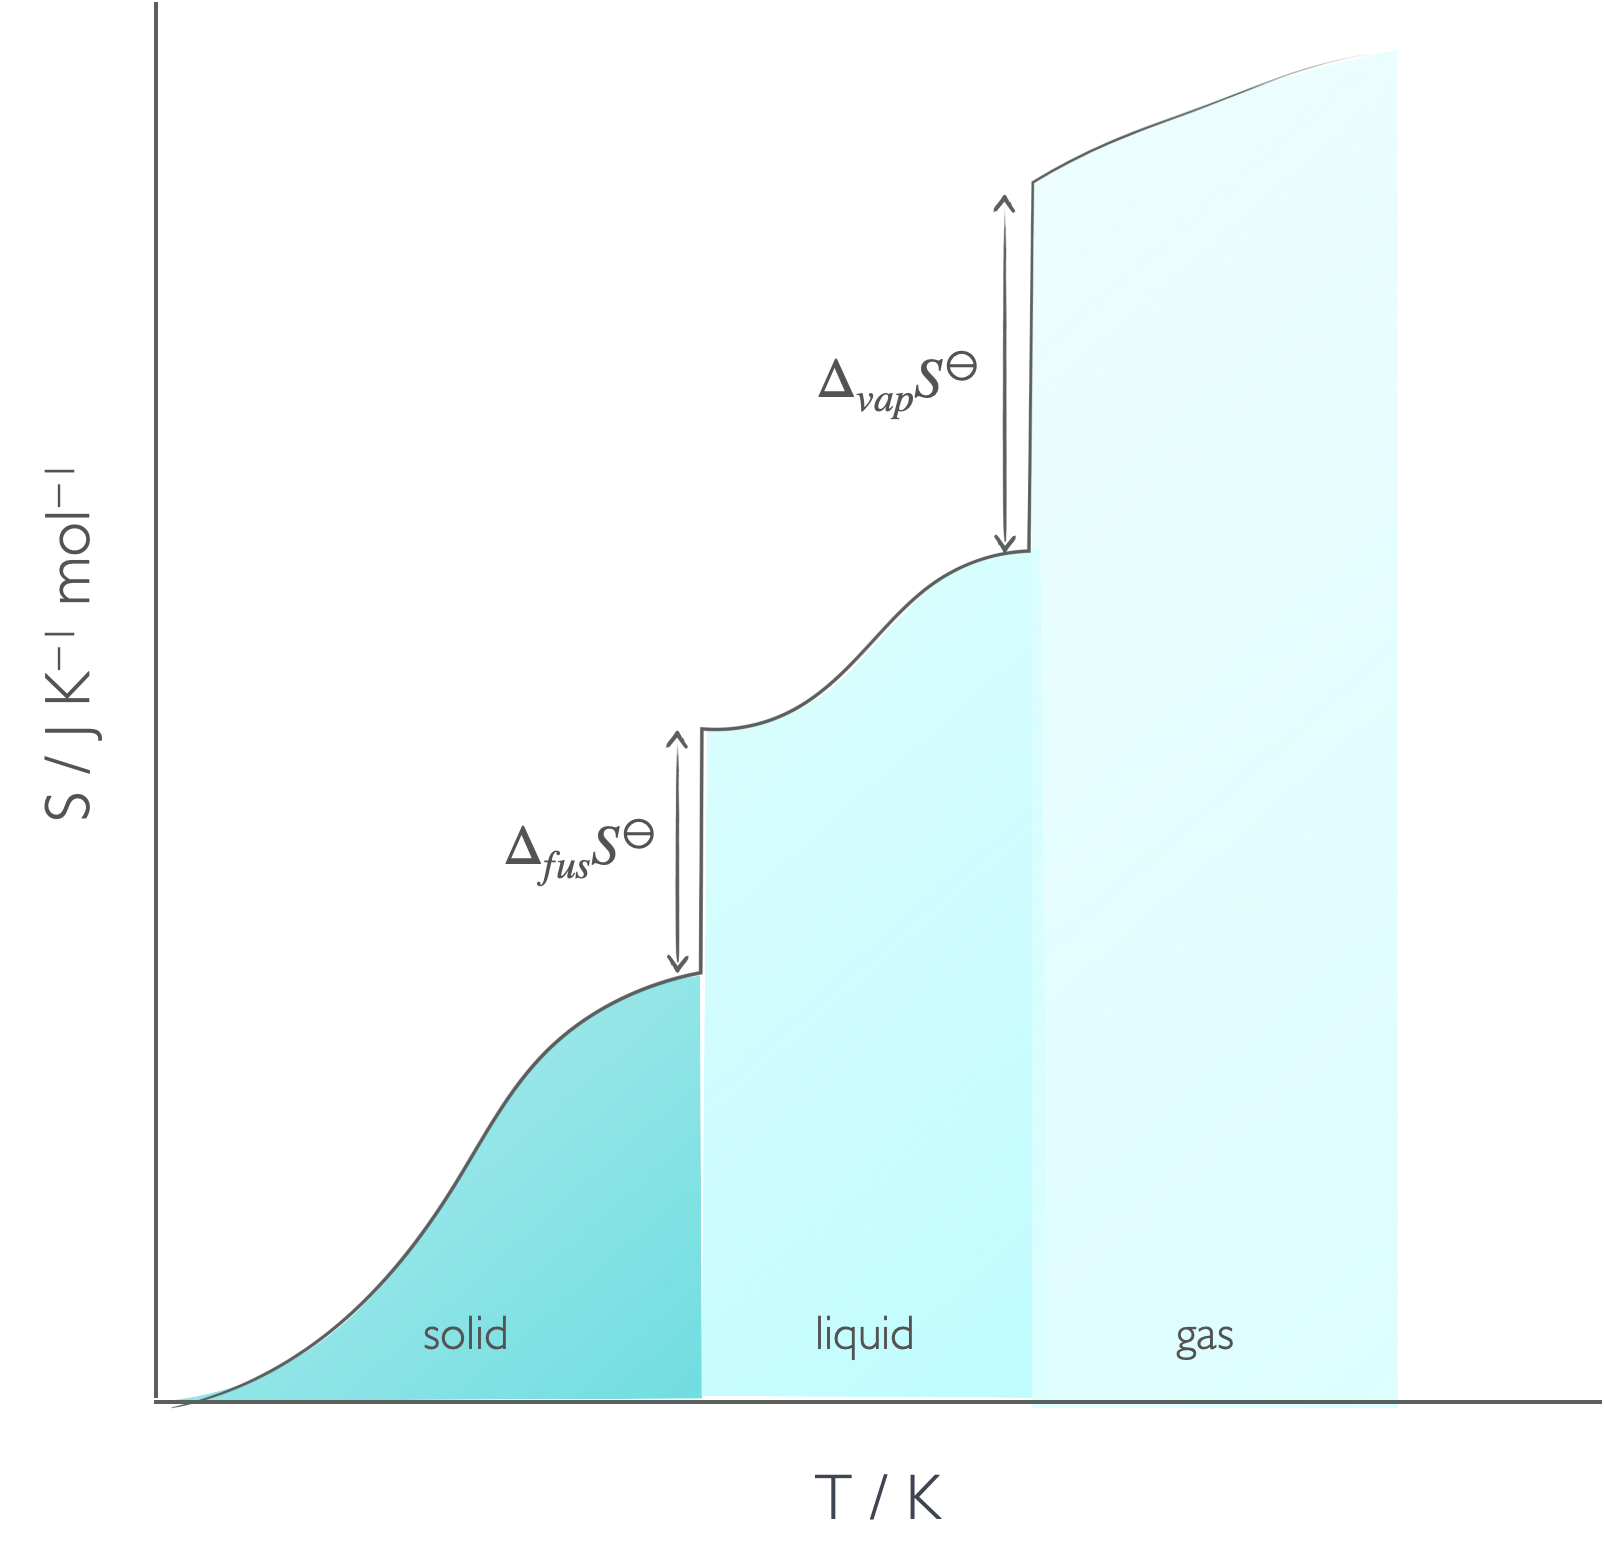
\includegraphics[width=0.8\linewidth]{images/entropyphase} 

}

\caption{The absolute entropy of a material has to consider the entropy of heating between absolute zero and the melting temperature, the entropy of fusion, the entropy between the melting temperature and boiling temperature, the entropy of vapourisation and then the entropy between the boiling temperature and final temperature.}\label{fig:entropyphase}
\end{figure}

\begin{equation}
S_m(T) = S_m(0)+ \int_0^{T_f}\frac{C_p(s)}{T}\textrm{d}T+ \frac{\Delta _{fus} H}{T_f}+ \int_{T_f}^{T_b}\frac{C_p(l)}{T}\textrm{d}T+ \frac{\Delta _{vap} H}{T_f}+ \int_{T_f}^T\frac{C_p(g)}{T}\textrm{d}T
\label{eq:entropyphase}
\end{equation}

From equation \eqref{eq:clausius} we can relate the enthalpy of phase change and entropy of phase change at constant pressure because phase changes are reversible processes.

\begin{equation}
\Delta_{vap} S=\frac{\Delta_{vap} H }{T_b}
\label{eq:entropyvap}
\end{equation}

\begin{equation}
\Delta_{fus} S=\frac{\Delta_{fus} H }{T_m}
\label{eq:entropyfus}
\end{equation}

\hypertarget{troutons-rule}{%
\subsection{Trouton's Rule}\label{troutons-rule}}

Trouton's rule is an empirical relationship which found that \(\frac{\Delta_{vap} H }{T_b}\) is around 85 J K\textsuperscript{−1} mol\textsuperscript{−1} for liquids that have no hydrogen bonding. For substances with hydrogen bonding \(\Delta_{vap} H\) is considerably higher because more heat is required to break all of the intermolecular bonds.

Equally some species have a lower than predicted entropy of vapourisation. These species may still have intermolecular bonding in the gas phase, such as formic acid which forms a molecular dimer at temperatures just above the boiling temperature (you can then see a `phase change' as this dimer dissociates at even higher temperatures). Otherwise it may be that the species is particularly `small' and has a low moment of rotational inertia, leading to large spacings in molecular energy levels and therefore relatively low entropy in the population of these levels.

\begin{longtable}[]{@{}cccc@{}}
\caption{\label{tab:trouton} Thermodynamic data for the vaporisation of a range of chemical species.}\tabularnewline
\toprule
\begin{minipage}[b]{0.22\columnwidth}\centering
\strut
\end{minipage} & \begin{minipage}[b]{0.22\columnwidth}\centering
\(\Delta_{vap} S^\ominus\) / J K\textsuperscript{−1} mol\textsuperscript{−1}\strut
\end{minipage} & \begin{minipage}[b]{0.22\columnwidth}\centering
\(\Delta_{vap} H^\ominus\) / kJ mol\textsuperscript{−1}\strut
\end{minipage} & \begin{minipage}[b]{0.22\columnwidth}\centering
\(T_b\) / K\strut
\end{minipage}\tabularnewline
\midrule
\endfirsthead
\toprule
\begin{minipage}[b]{0.22\columnwidth}\centering
\strut
\end{minipage} & \begin{minipage}[b]{0.22\columnwidth}\centering
\(\Delta_{vap} S^\ominus\) / J K\textsuperscript{−1} mol\textsuperscript{−1}\strut
\end{minipage} & \begin{minipage}[b]{0.22\columnwidth}\centering
\(\Delta_{vap} H^\ominus\) / kJ mol\textsuperscript{−1}\strut
\end{minipage} & \begin{minipage}[b]{0.22\columnwidth}\centering
\(T_b\) / K\strut
\end{minipage}\tabularnewline
\midrule
\endhead
\begin{minipage}[t]{0.22\columnwidth}\centering
benzene\strut
\end{minipage} & \begin{minipage}[t]{0.22\columnwidth}\centering
87.2\strut
\end{minipage} & \begin{minipage}[t]{0.22\columnwidth}\centering
30.8\strut
\end{minipage} & \begin{minipage}[t]{0.22\columnwidth}\centering
353.2\strut
\end{minipage}\tabularnewline
\begin{minipage}[t]{0.22\columnwidth}\centering
bromine\strut
\end{minipage} & \begin{minipage}[t]{0.22\columnwidth}\centering
88.6\strut
\end{minipage} & \begin{minipage}[t]{0.22\columnwidth}\centering
29.45\strut
\end{minipage} & \begin{minipage}[t]{0.22\columnwidth}\centering
332.4\strut
\end{minipage}\tabularnewline
\begin{minipage}[t]{0.22\columnwidth}\centering
tetrachloromethane\strut
\end{minipage} & \begin{minipage}[t]{0.22\columnwidth}\centering
85.9\strut
\end{minipage} & \begin{minipage}[t]{0.22\columnwidth}\centering
30.00\strut
\end{minipage} & \begin{minipage}[t]{0.22\columnwidth}\centering
349.9\strut
\end{minipage}\tabularnewline
\begin{minipage}[t]{0.22\columnwidth}\centering
hydrogen sulphide\strut
\end{minipage} & \begin{minipage}[t]{0.22\columnwidth}\centering
87.9\strut
\end{minipage} & \begin{minipage}[t]{0.22\columnwidth}\centering
18.67\strut
\end{minipage} & \begin{minipage}[t]{0.22\columnwidth}\centering
212.8\strut
\end{minipage}\tabularnewline
\begin{minipage}[t]{0.22\columnwidth}\centering
mercury\strut
\end{minipage} & \begin{minipage}[t]{0.22\columnwidth}\centering
94.2\strut
\end{minipage} & \begin{minipage}[t]{0.22\columnwidth}\centering
59.30\strut
\end{minipage} & \begin{minipage}[t]{0.22\columnwidth}\centering
692.7\strut
\end{minipage}\tabularnewline
\begin{minipage}[t]{0.22\columnwidth}\centering
ammonia\strut
\end{minipage} & \begin{minipage}[t]{0.22\columnwidth}\centering
97.4\strut
\end{minipage} & \begin{minipage}[t]{0.22\columnwidth}\centering
23.4\strut
\end{minipage} & \begin{minipage}[t]{0.22\columnwidth}\centering
239.7\strut
\end{minipage}\tabularnewline
\begin{minipage}[t]{0.22\columnwidth}\centering
water\strut
\end{minipage} & \begin{minipage}[t]{0.22\columnwidth}\centering
109.1\strut
\end{minipage} & \begin{minipage}[t]{0.22\columnwidth}\centering
40.7\strut
\end{minipage} & \begin{minipage}[t]{0.22\columnwidth}\centering
373.2\strut
\end{minipage}\tabularnewline
\begin{minipage}[t]{0.22\columnwidth}\centering
methane\strut
\end{minipage} & \begin{minipage}[t]{0.22\columnwidth}\centering
73.2\strut
\end{minipage} & \begin{minipage}[t]{0.22\columnwidth}\centering
8.18\strut
\end{minipage} & \begin{minipage}[t]{0.22\columnwidth}\centering
111.7\strut
\end{minipage}\tabularnewline
\begin{minipage}[t]{0.22\columnwidth}\centering
argon\strut
\end{minipage} & \begin{minipage}[t]{0.22\columnwidth}\centering
74.4\strut
\end{minipage} & \begin{minipage}[t]{0.22\columnwidth}\centering
6.5\strut
\end{minipage} & \begin{minipage}[t]{0.22\columnwidth}\centering
87.3\strut
\end{minipage}\tabularnewline
\begin{minipage}[t]{0.22\columnwidth}\centering
formic acid\strut
\end{minipage} & \begin{minipage}[t]{0.22\columnwidth}\centering
61.8\strut
\end{minipage} & \begin{minipage}[t]{0.22\columnwidth}\centering
23.1\strut
\end{minipage} & \begin{minipage}[t]{0.22\columnwidth}\centering
373.9\strut
\end{minipage}\tabularnewline
\bottomrule
\end{longtable}

\hypertarget{residual-entropy}{%
\section{Residual entropy}\label{residual-entropy}}

As we cool our sample you would expect that as the temperature reaches absolute zero you would expect the entropy to fall to zero, however under some circumstances there may still be multiple possible ways of arranging a system. These include:

\begin{itemize}
\tightlist
\item
  isotopes being randomly distributed in a sample
\item
  systems where there is no enthalpy change for different arrangements, such as CO
\item
  degeneracy in ground state
\end{itemize}

\begin{figure}

{\centering 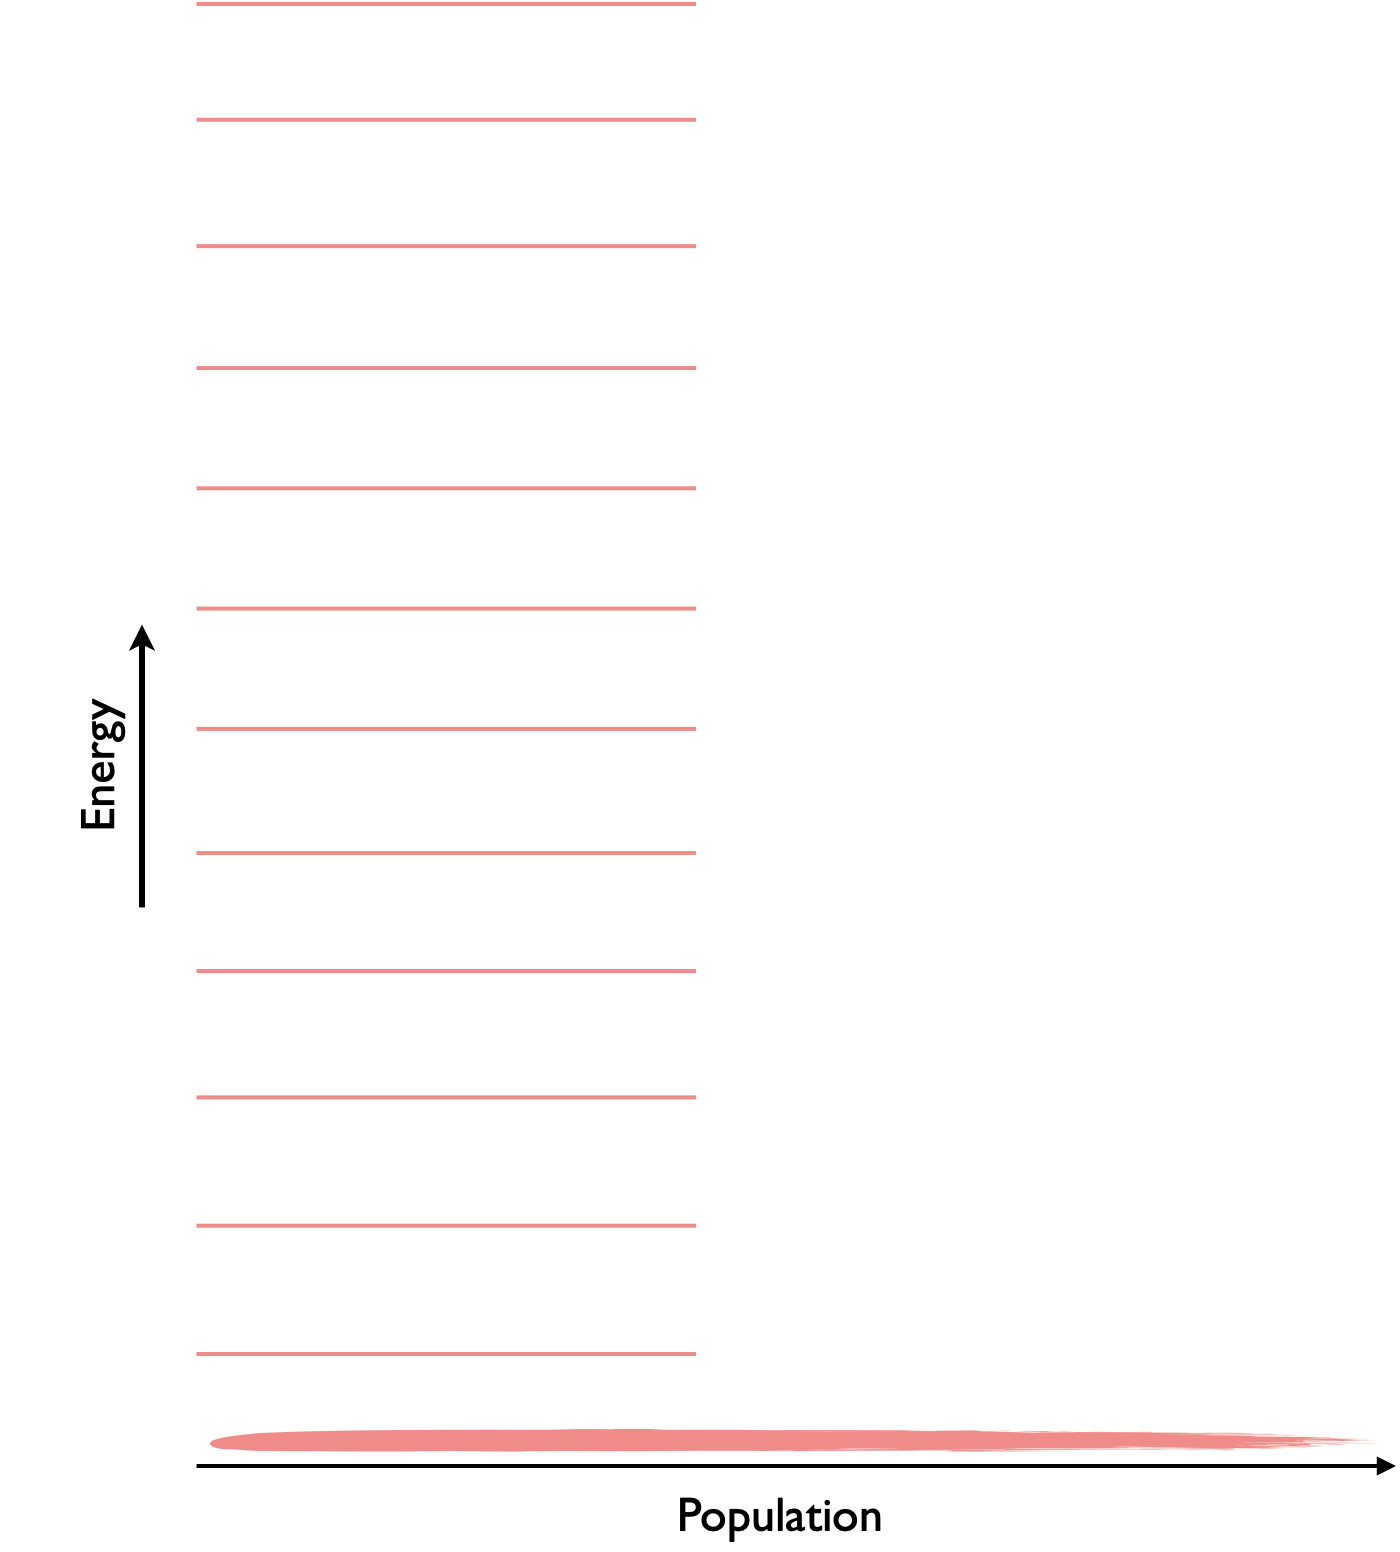
\includegraphics[width=0.8\linewidth]{images/entropyzero} 

}

\caption{If we follow our molecular understanding of entropy from Boltzmann we could theoretically reach a point with zero entropy where all molcules are in the same state.}\label{fig:entropyzero}
\end{figure}

\begin{figure}

{\centering 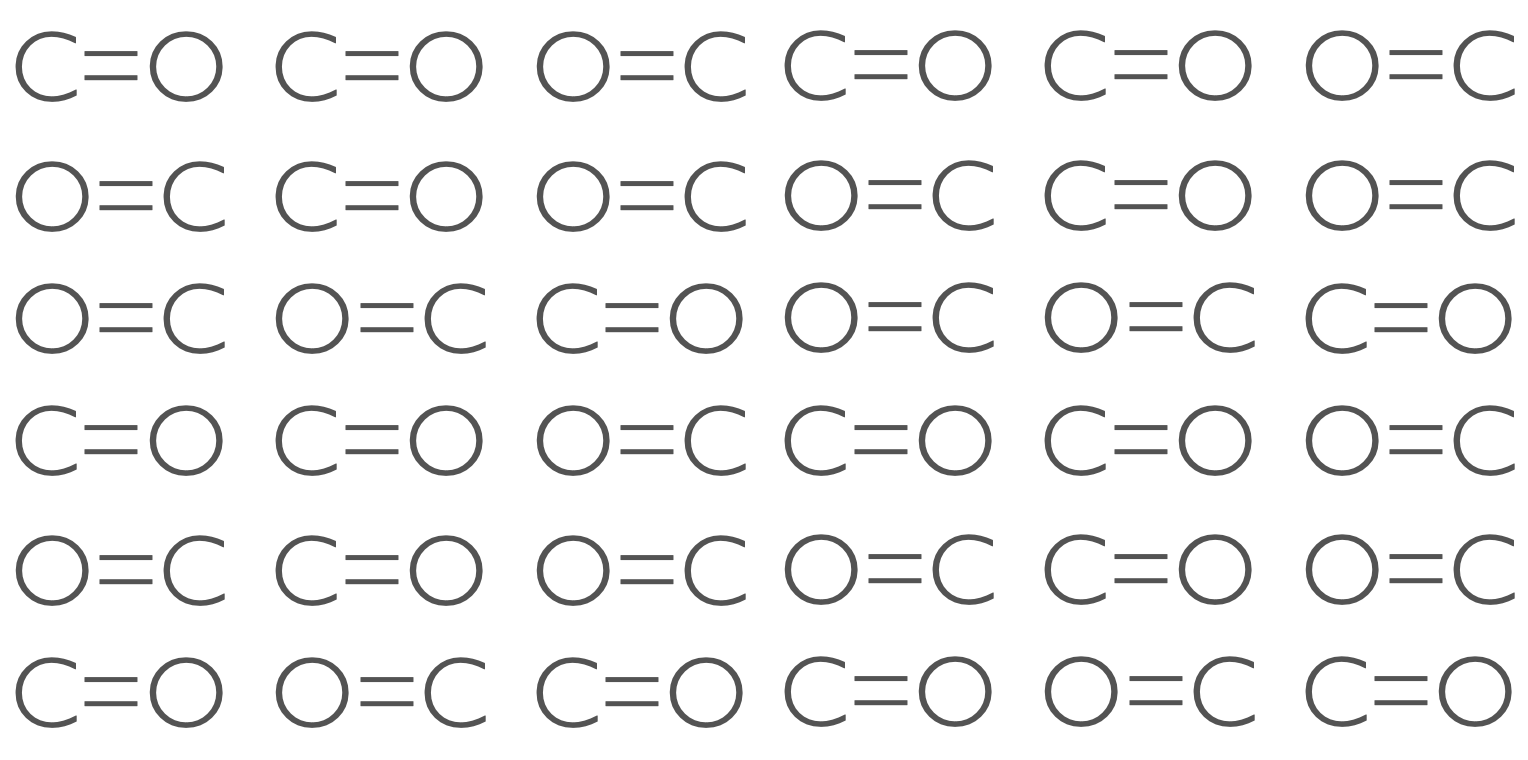
\includegraphics[width=0.8\linewidth]{images/CO} 

}

\caption{CO molecules can exist in one of two states (C=O and O=C) and because ther eis a very even electic charge across the molecule the two states are degenerate in energy and two possible microstates exist for each CO site in the crystal.}\label{fig:CO}
\end{figure}

We can calculate the residual entropy using the statistical definition of entropy (equation \eqref{eq:boltzmann}).

\hypertarget{entropy-changes-for-isothermal-expansion-of-a-gas}{%
\section{Entropy changes for isothermal expansion of a gas}\label{entropy-changes-for-isothermal-expansion-of-a-gas}}

If we think about entropy of the probabiity of a given state being achieved then as the `box' gets bigger the probability of a particle being in any position falls and so the entropy of the system increases.

\begin{figure}

{\centering 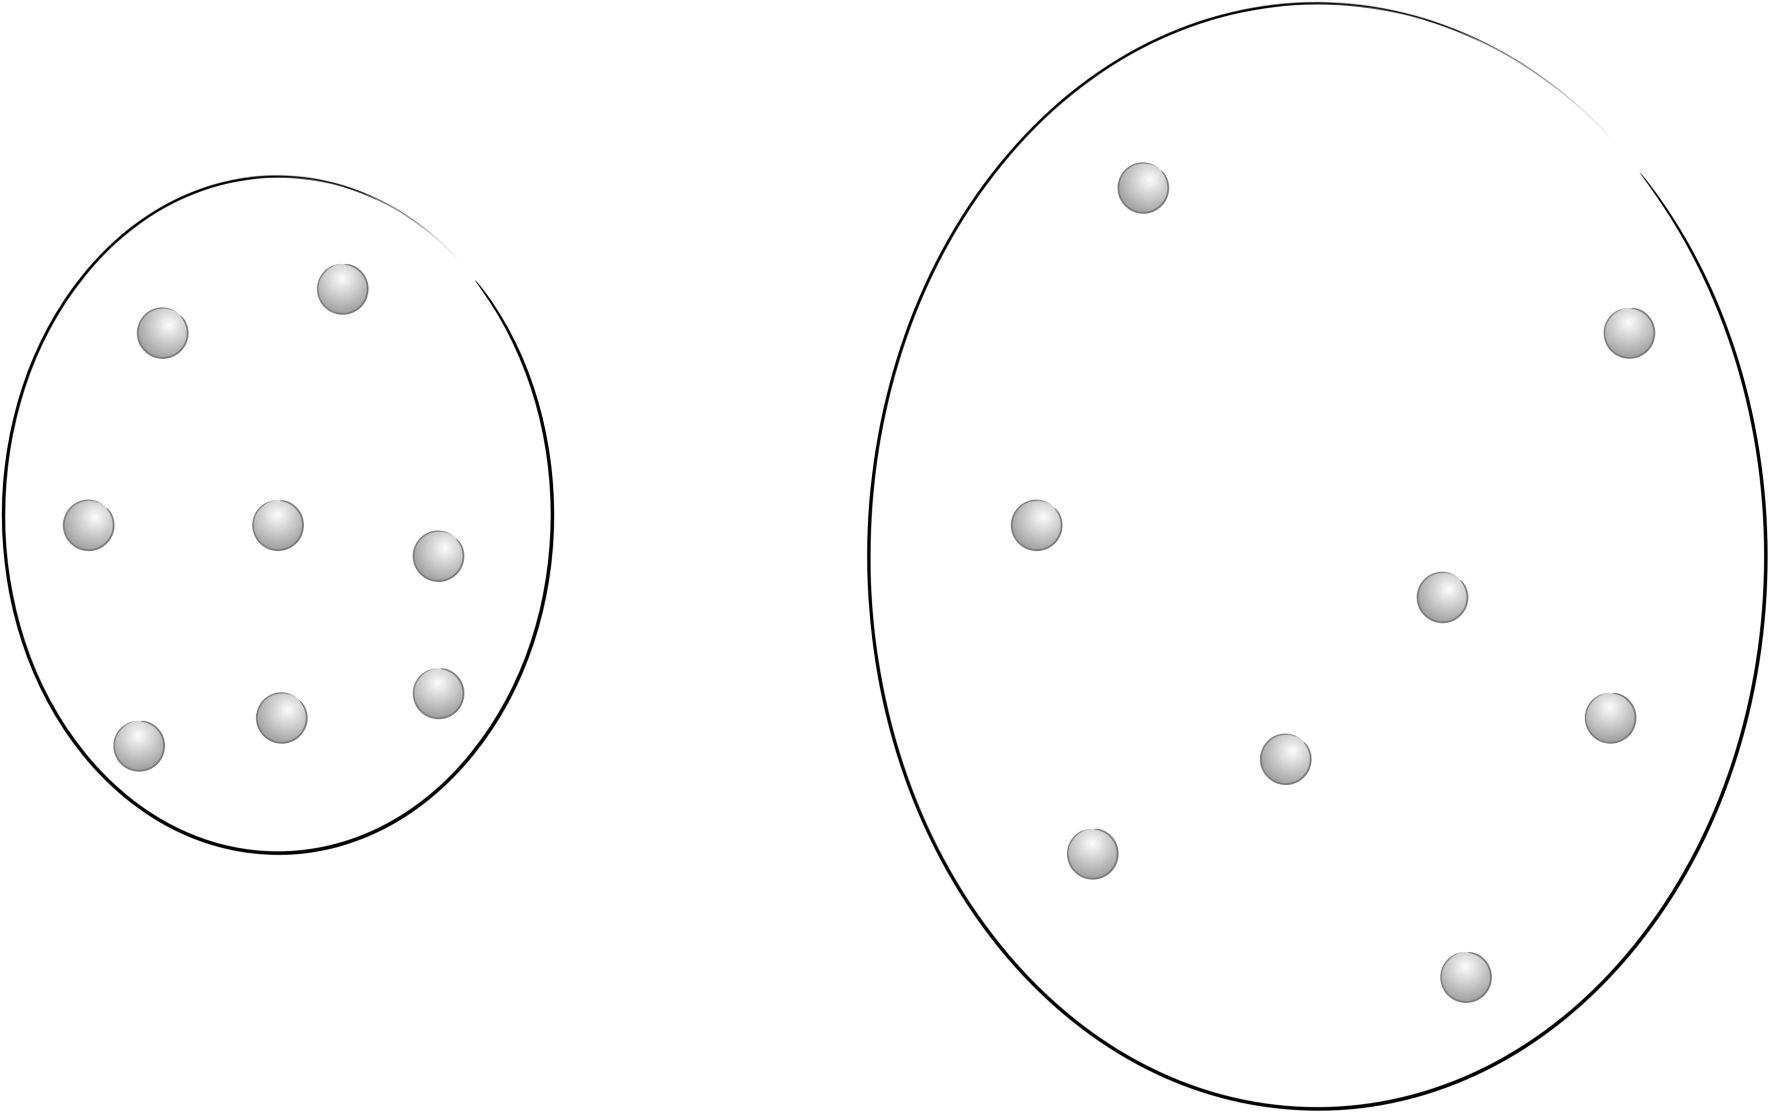
\includegraphics[width=0.8\linewidth]{images/entropyexpansion} 

}

\caption{As the container expands the molecules have more possible positions and so the probability of a particle being in any single postion is reduced and the entropy increases.}\label{fig:entropyexpansion}
\end{figure}

If we actually think about the energy levels in the system, we know that the occupation of these levels follows the Maxwell-Boltzmann distribution (equation \eqref{eq:maxwell}) when the levels are spaced further apart, fewer macrostates are occupied and so the probability of finding a particle in any state is relatively high. As the energy levels get closer together the probability of finding a particle in any given level decreases and so the entropy of the system increases.

\begin{figure}

{\centering 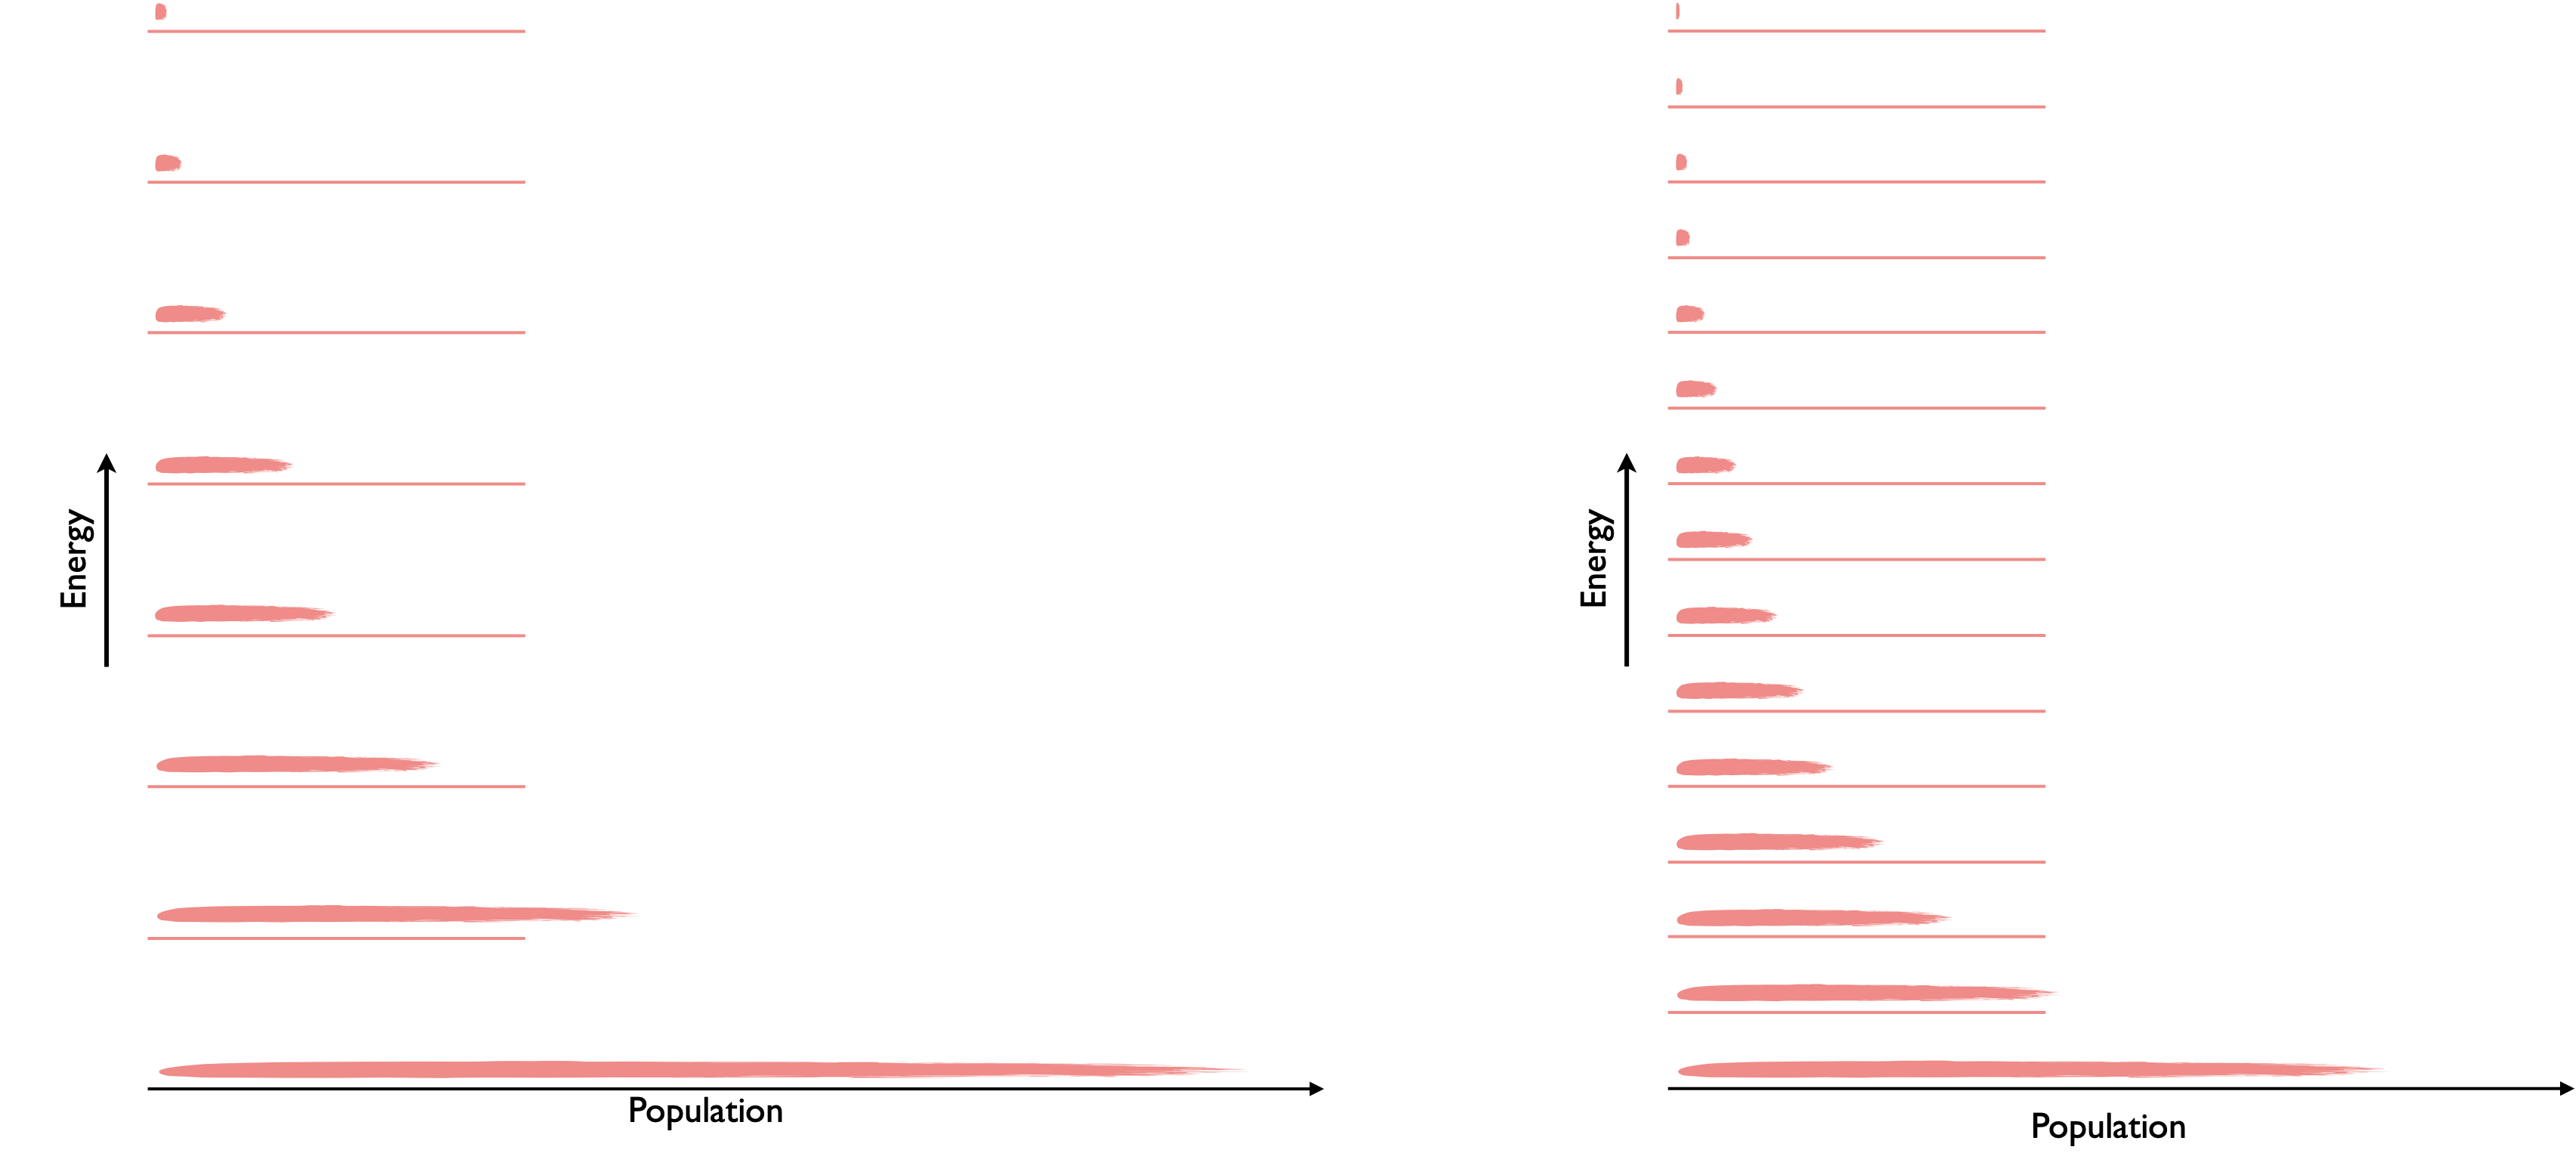
\includegraphics[width=0.8\linewidth]{images/boxlevels} 

}

\caption{According to the particle in a box model energy levels in a small box (left) are spaced further apart than those in a larger box.}\label{fig:boxlevels}
\end{figure}

Now if we consider the entropy change in an isothermal expansion then:

\begin{equation}
\Delta S=nR \ln\frac{V_\textrm{f}}{V_\textrm{i}}
\label{eq:entropyexpansion}
\end{equation}

This equation is derived from our expression of work done in a reversible expansion, and the relationship between heat and work when that expansion is isothermal. Combining this with our definition of entropy (\eqref{eq:clausiusineq}) gives us this expression above.

\hypertarget{sec:w3p2question}{%
\section{Questions}\label{sec:w3p2question}}

\begin{enumerate}
\def\labelenumi{\arabic{enumi}.}
\item
  Calculate the change of entropy change when exactly 1 mol of methanol is heated at constant pressure from 5 °C to 35 °C, the molar heat capacity, C\textsubscript{p}, of methanol is 81.6 J K\textsuperscript{−1} mol\textsuperscript{−1}, assume that the molar heat capacity, C\textsubscript{p} is constant over this temperature range.
\item
  Calculate the entropy change of cooling of liquid mercury from 25 ºC to 0 ºC. (C\textsubscript{p} = 27.98 J K\textsuperscript{−1} mol\textsuperscript{−1})
\item
  Calculate the change in entropy of 5.151 mol of a perfect gas when it is compressed isothermally to 59.8 \% of its initial volume.
\item
  Use the following data to calculate the reaction entropy at 298 K for the thermal decomposition of 2.651 g of ammonium chloride, NH\textsubscript{4}Cl
\end{enumerate}

NH\textsubscript{4}Cl(s) → NH\textsubscript{3}(g) + HCl(g)

\begin{longtable}[]{@{}cc@{}}
\toprule
& Sm° / J K\textsuperscript{−1} mol\textsuperscript{−1}\tabularnewline
\midrule
\endhead
NH\textsubscript{4}Cl(s) & 94.85\tabularnewline
NH3(g) & 192.77\tabularnewline
HCl(g) & 186.90\tabularnewline
\bottomrule
\end{longtable}

\begin{enumerate}
\def\labelenumi{\arabic{enumi}.}
\setcounter{enumi}{4}
\tightlist
\item
  If the specific heat of water is 4.184 J K\textsuperscript{−1} g\textsuperscript{−1} what is the change in entropy when water is heated from 20 ºC and 80 ºC?
\end{enumerate}

\hypertarget{sec:w3p2ans}{%
\section{Answers}\label{sec:w3p2ans}}

\begin{enumerate}
\def\labelenumi{\arabic{enumi}.}
\item
  \(\Delta S=\) 8.36 J K\textsuperscript{−1} mol\textsuperscript{−1}
\item
  \(\Delta S=\) −2.45 J K\textsuperscript{−1} mol\textsuperscript{−1}
\item
  \(\Delta S=\) -22.02 J K\textsuperscript{−1}
\item
  \(\Delta S=\) +14.11 J K\textsuperscript{−1}
\item
  \(\Delta S=\) 14.0 J K\textsuperscript{−1} mol\textsuperscript{−1}
\end{enumerate}

\hypertarget{ch:Part7}{%
\chapter{Week 4 - Part 1}\label{ch:Part7}}

\hypertarget{gibbs-free-energy}{%
\section{Gibbs' free energy}\label{gibbs-free-energy}}

You will recall from section \ref{sec:2ndlaw} that the entropy of a universe has to increase in any spontaneous change. Equation \eqref{eq:clausius}, linked the entropy, \(\Delta S\), to the heat provided to the system reversibly, \$q\_\{\textrm{rev}\}. Consequently, since the heat lost from the surroundings and the heat gained by the system are the same, at constant pressure we can say:

\begin{equation}
\Delta S_{sur}=-\frac {\Delta H}{T}
\label{eq:entropysurrounding}
\end{equation}

J.W. Gibbs' contribution to thermodynamics was recognising that the entropy change of the universe was the sum of the entropy of the system and surroundings, and by using the relationship in equation \eqref{eq:entropysurrounding} the total entropy of the universe can be definied solely in terms of the thermodynamics of the system. Gibbs went on further to define the Gibbs' free energy, \(\Delta G\) as \(\Delta G = - T\Delta S_{\textrm{total}}\).

This gives one of the most important equations in science, the Gibbs' equation:

\begin{equation}
\Delta G^\ominus = \Delta H^\ominus - T \Delta S^\ominus
\label{eq:Gibbs}
\end{equation}

Since enthalpy, entropy and temperature are all state functions so is the Gibbs' free energy, which we have already seen in section \ref{sec:equations1}, equation \eqref{eq:Gibbsstate}.

The free energy of a system is a measure of a system's ability to do (non-expansion) work.

\hypertarget{helmholtz-free-energy}{%
\subsection{Helmholtz free energy}\label{helmholtz-free-energy}}

There is an equivalent function called the Helmholtz free energy (\(A\) and \(\Delta A\) for changes), which is a measure of the free energy at constant volume, whilst I am mentioning it here in chemistry it is more usual to consider the Gibbs' free energy.

\begin{equation}
\Delta G = \Delta H - T \Delta S
\label{eq:Helmholtz}
\end{equation}

\hypertarget{factors-affecting-the-gibbs-free-energy}{%
\subsection{Factors affecting the Gibbs free energy}\label{factors-affecting-the-gibbs-free-energy}}

The Gibbs' equation makes it fairly clear that the Gibbs' energy depends upon temperature.

\begin{longtable}[]{@{}cccc@{}}
\caption{\label{tab:Gibbstemp} The spontaneity of a reaction at different temperatures.}\tabularnewline
\toprule
\(\Delta H\) & \(\Delta S\) & \(\Delta G\) & Spontaneity\tabularnewline
\midrule
\endfirsthead
\toprule
\(\Delta H\) & \(\Delta S\) & \(\Delta G\) & Spontaneity\tabularnewline
\midrule
\endhead
+ endothermic & + & + at low T − at high T & spontaneous at high temperature\tabularnewline
+ endothermic & − & + & needs work to occur\tabularnewline
− exothermic & + & − & always spontaneous\tabularnewline
− exothermic & − & − at low T + at high T & spontaneous at low temperature\tabularnewline
\bottomrule
\end{longtable}

\begin{figure}

{\centering 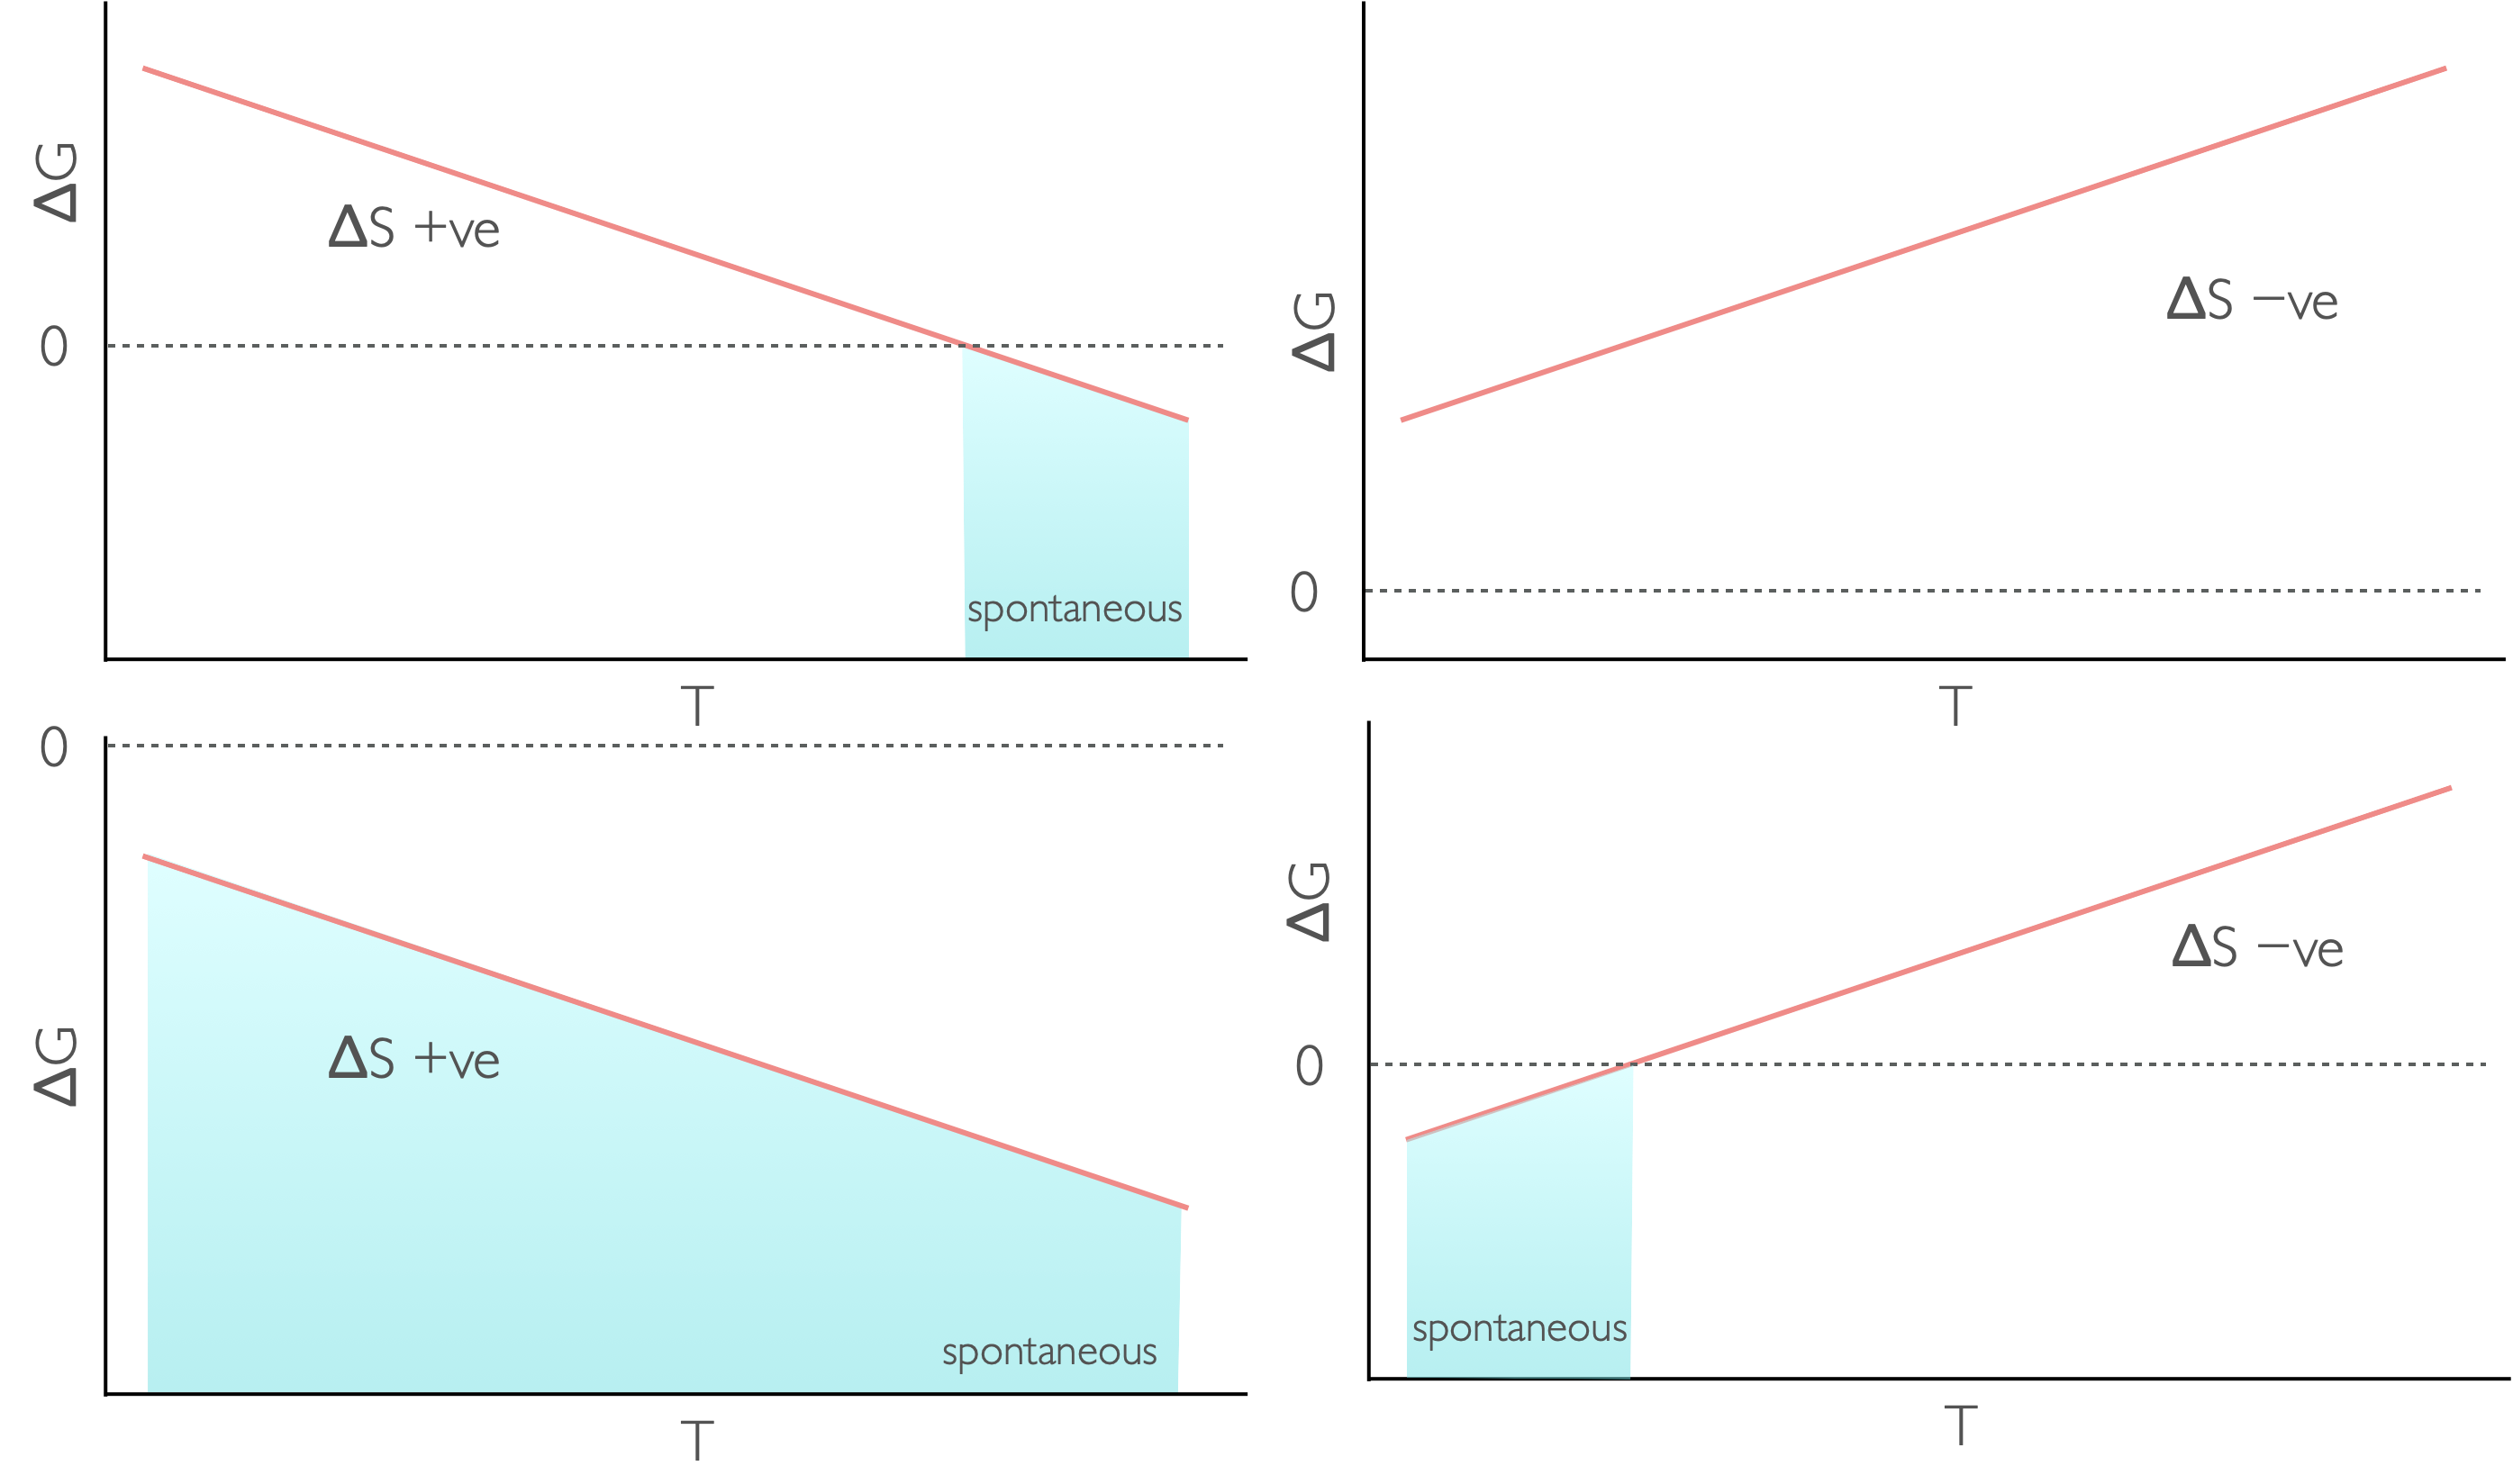
\includegraphics[width=0.8\linewidth]{images/Gibbstemp} 

}

\caption{The temperature dependence of Gibbs free energy for different reaction types: endothermic and increase in entropy (top left), endothermic with a decrease in entropy (top right), exothermic with an increase in entropy (bottom left) and exothermix with a decrease in entropy (bottom right).}\label{fig:Gibbstemp}
\end{figure}

We can derive an expression which shows that the Gibbs' free energy depends only upon the pressure and temperature of a system:

\begin{equation*}
\textrm{d}G= -S\textrm{d}T + V\textrm{d}p
\end{equation*}

This result is already known to you as it is the basis of phase diagrams (section \ref{sec:phasegibbs}).

\hypertarget{dilution}{%
\subsection{Dilution}\label{dilution}}

The entropy change of dilution is given by:

\begin{equation*}
\Delta S = R \ln \frac{c_i}{c_f}
\end{equation*}

This makes sense as it is similar to equation \eqref{eq:entropyexpansion}, for the entropy change of expansion, but high concentrations occur at low volumes and so the terms are switched.

Consequently if the enthalpy of dilution is 0, (which is normally though not always the case), this means the Gibbs energy change of dilution is:

\begin{equation}
\Delta G = RT \ln \frac{c_f}{c_i}
\label{eq:Gibbsdilution}
\end{equation}

\hypertarget{sec:phasegibbs}{%
\section{Phase changes}\label{sec:phasegibbs}}

\begin{figure}

{\centering 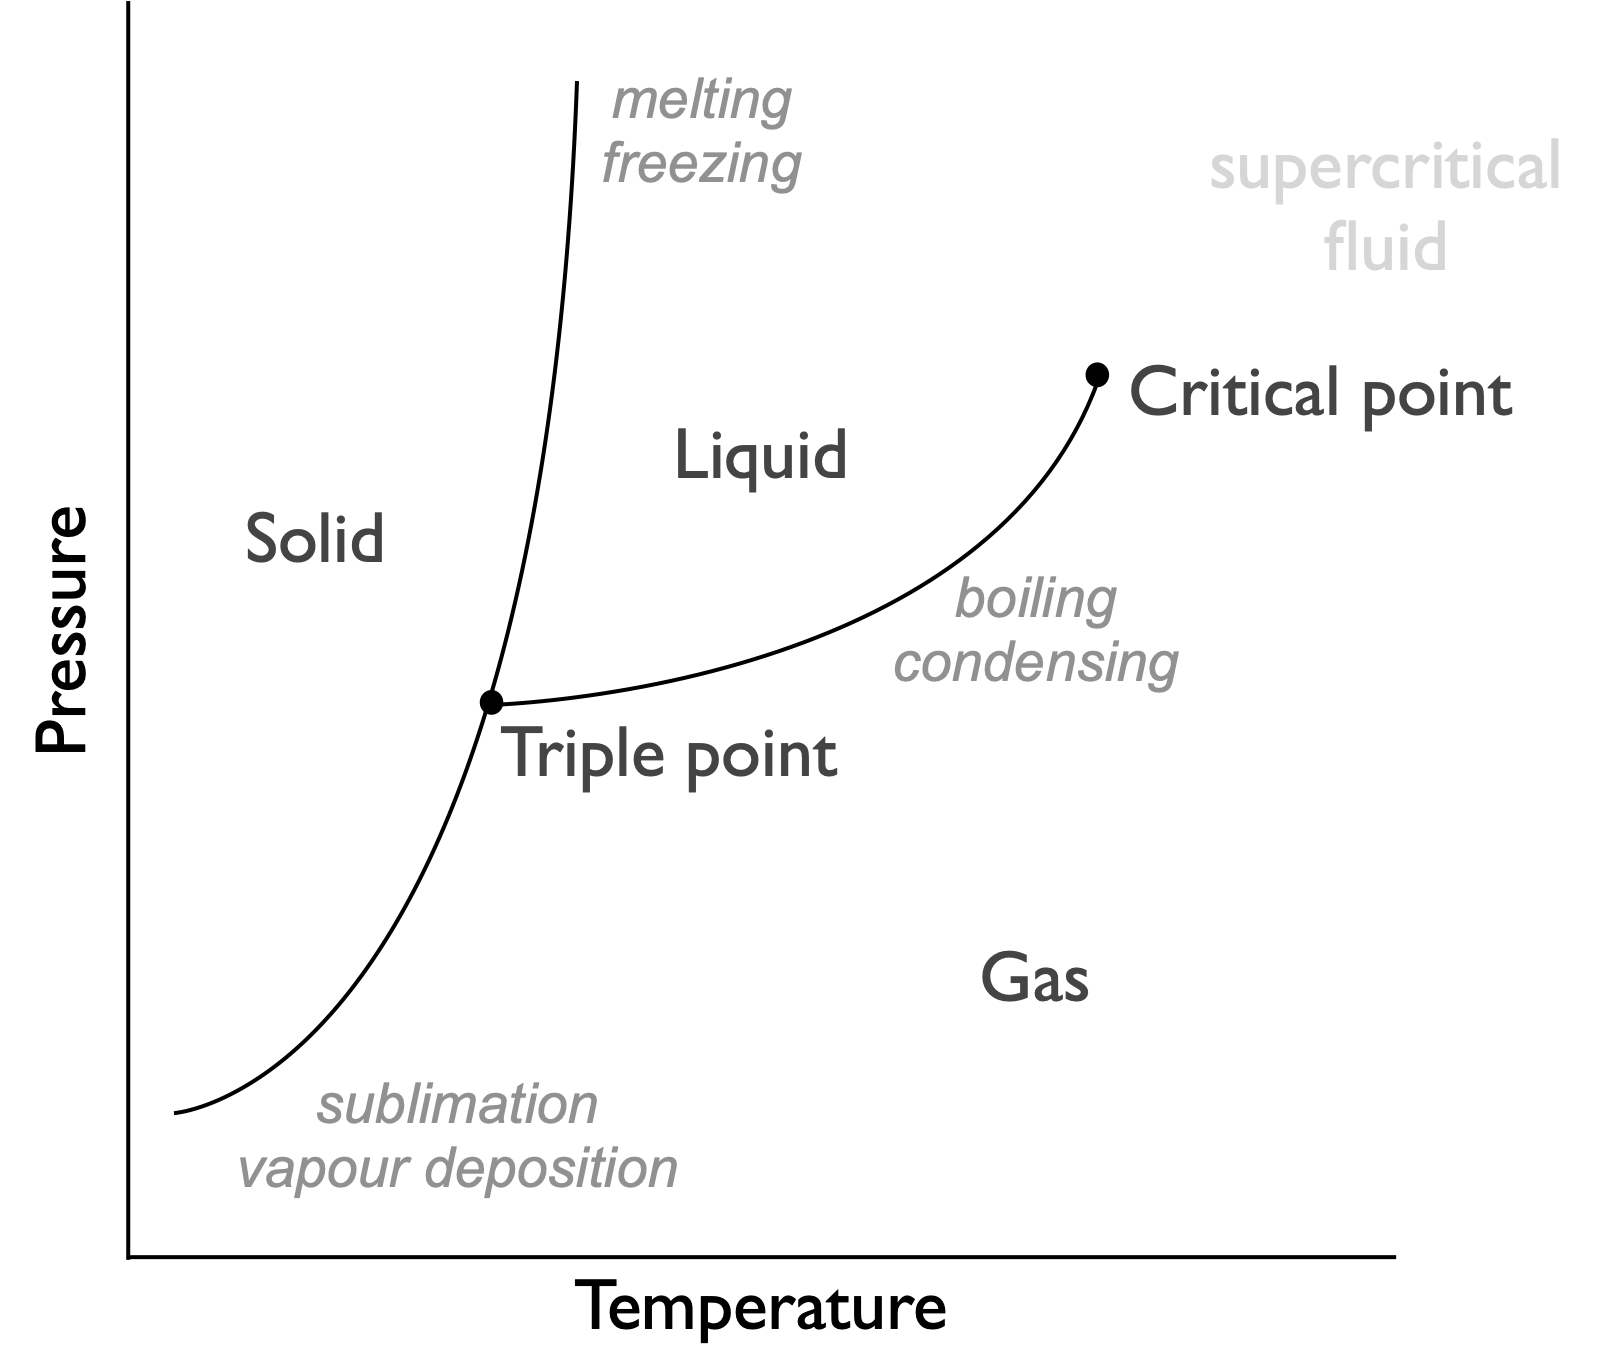
\includegraphics[width=0.8\linewidth]{images/phasediagram} 

}

\caption{Phase diagram for a typical system, indicating phases are functions of pressure and temperature. This is because the favoured phase is definied by the Gibbs free energy of the system}\label{fig:phasediagram}
\end{figure}

A phase diagram is actually a figure showing which phase has the lowest Gibbs' free energy, at phase boundaries the values of Gibbs' free energy for the two phases are identical and they are in equilibrium. The phase diagrams show that there is both a pressure and temperature dependance of the Gibbs' free energy.

\begin{figure}

{\centering 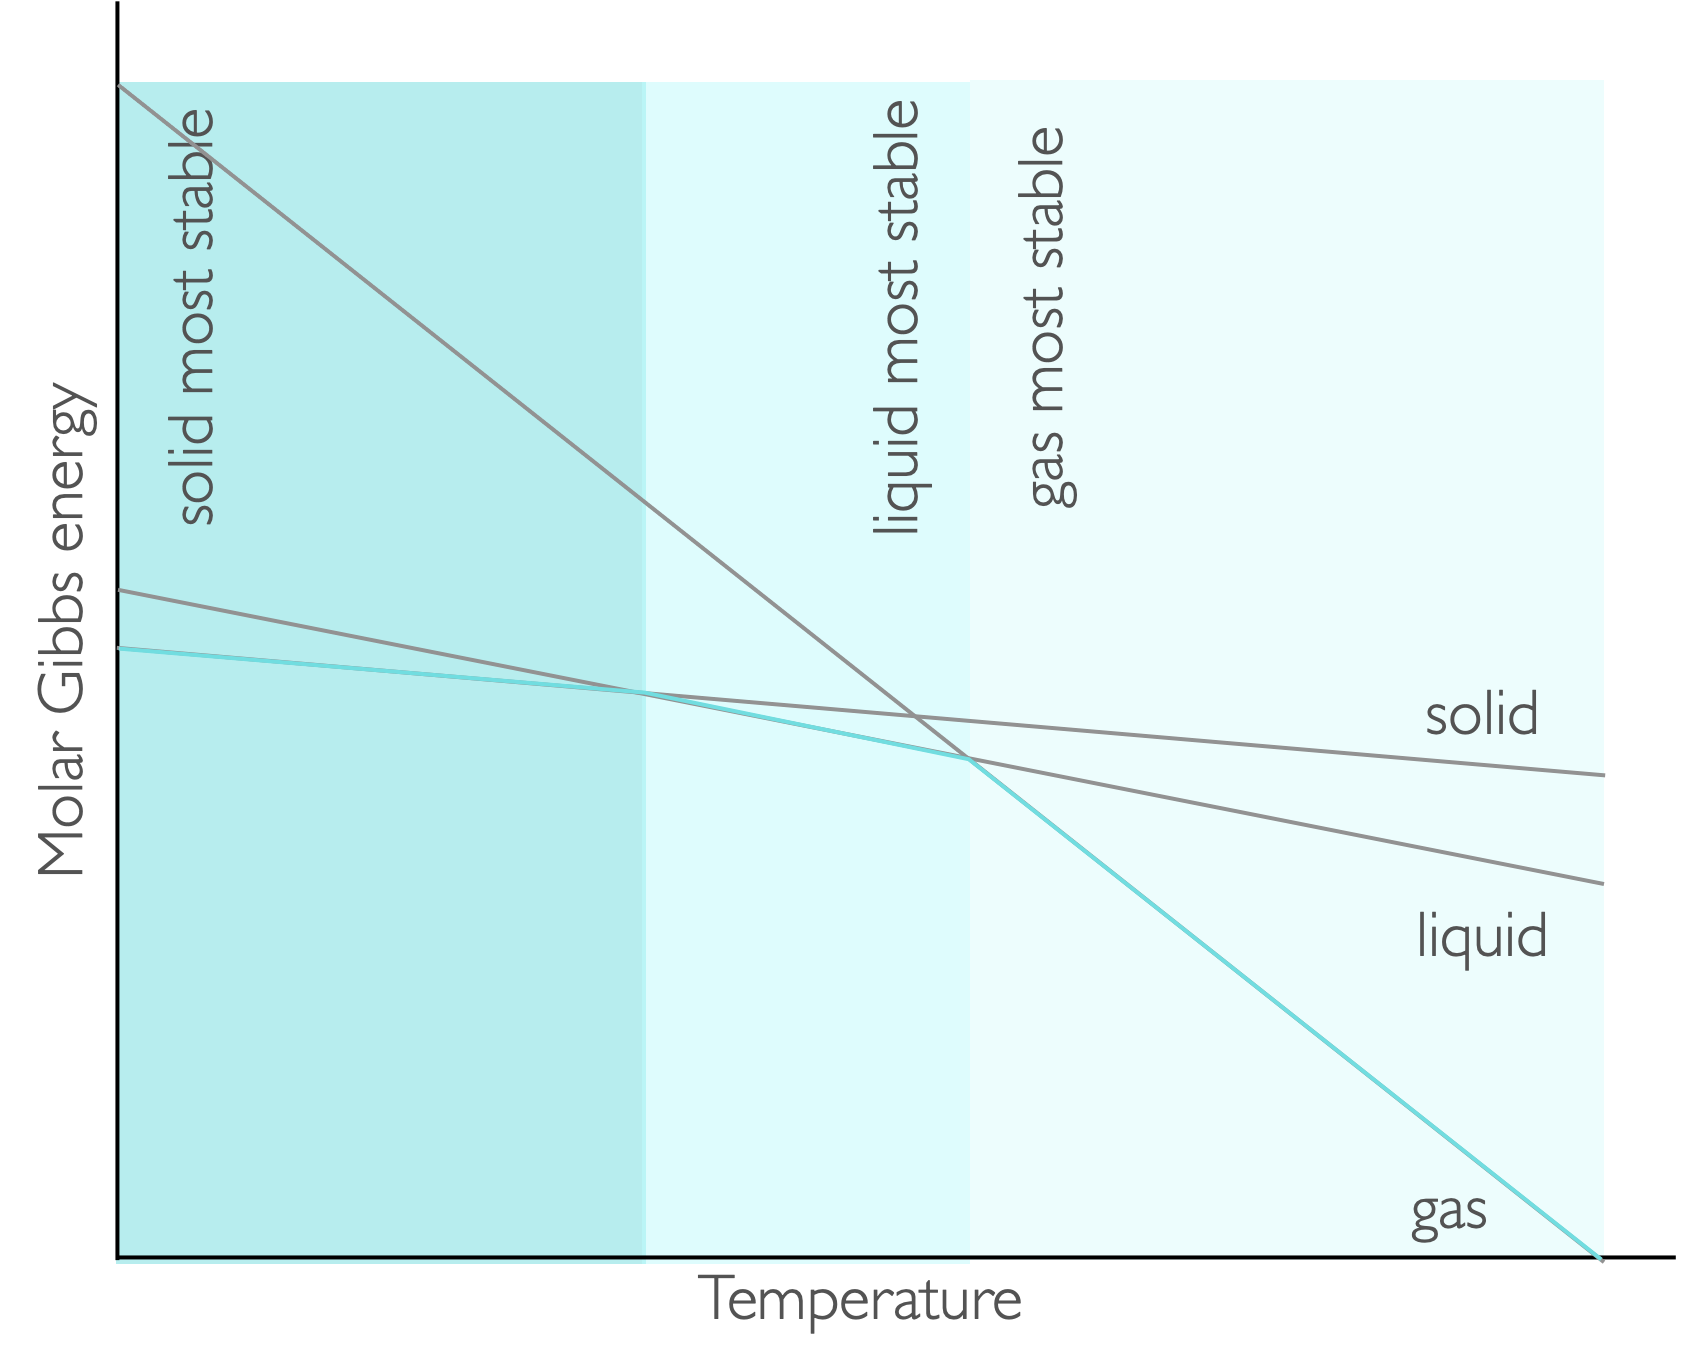
\includegraphics[width=0.8\linewidth]{images/gibbstempstate} 

}

\caption{The gradient of each line on a plot of Gibbs free energy against temperature is −S, consequently at low temperatures teh solid has the lowest value of molar Gibbs energy at low temperature and that phase is favoured, as the temperature is increased teh liquid and then the gas are favoured}\label{fig:gibbstempstate}
\end{figure}

\begin{figure}

{\centering 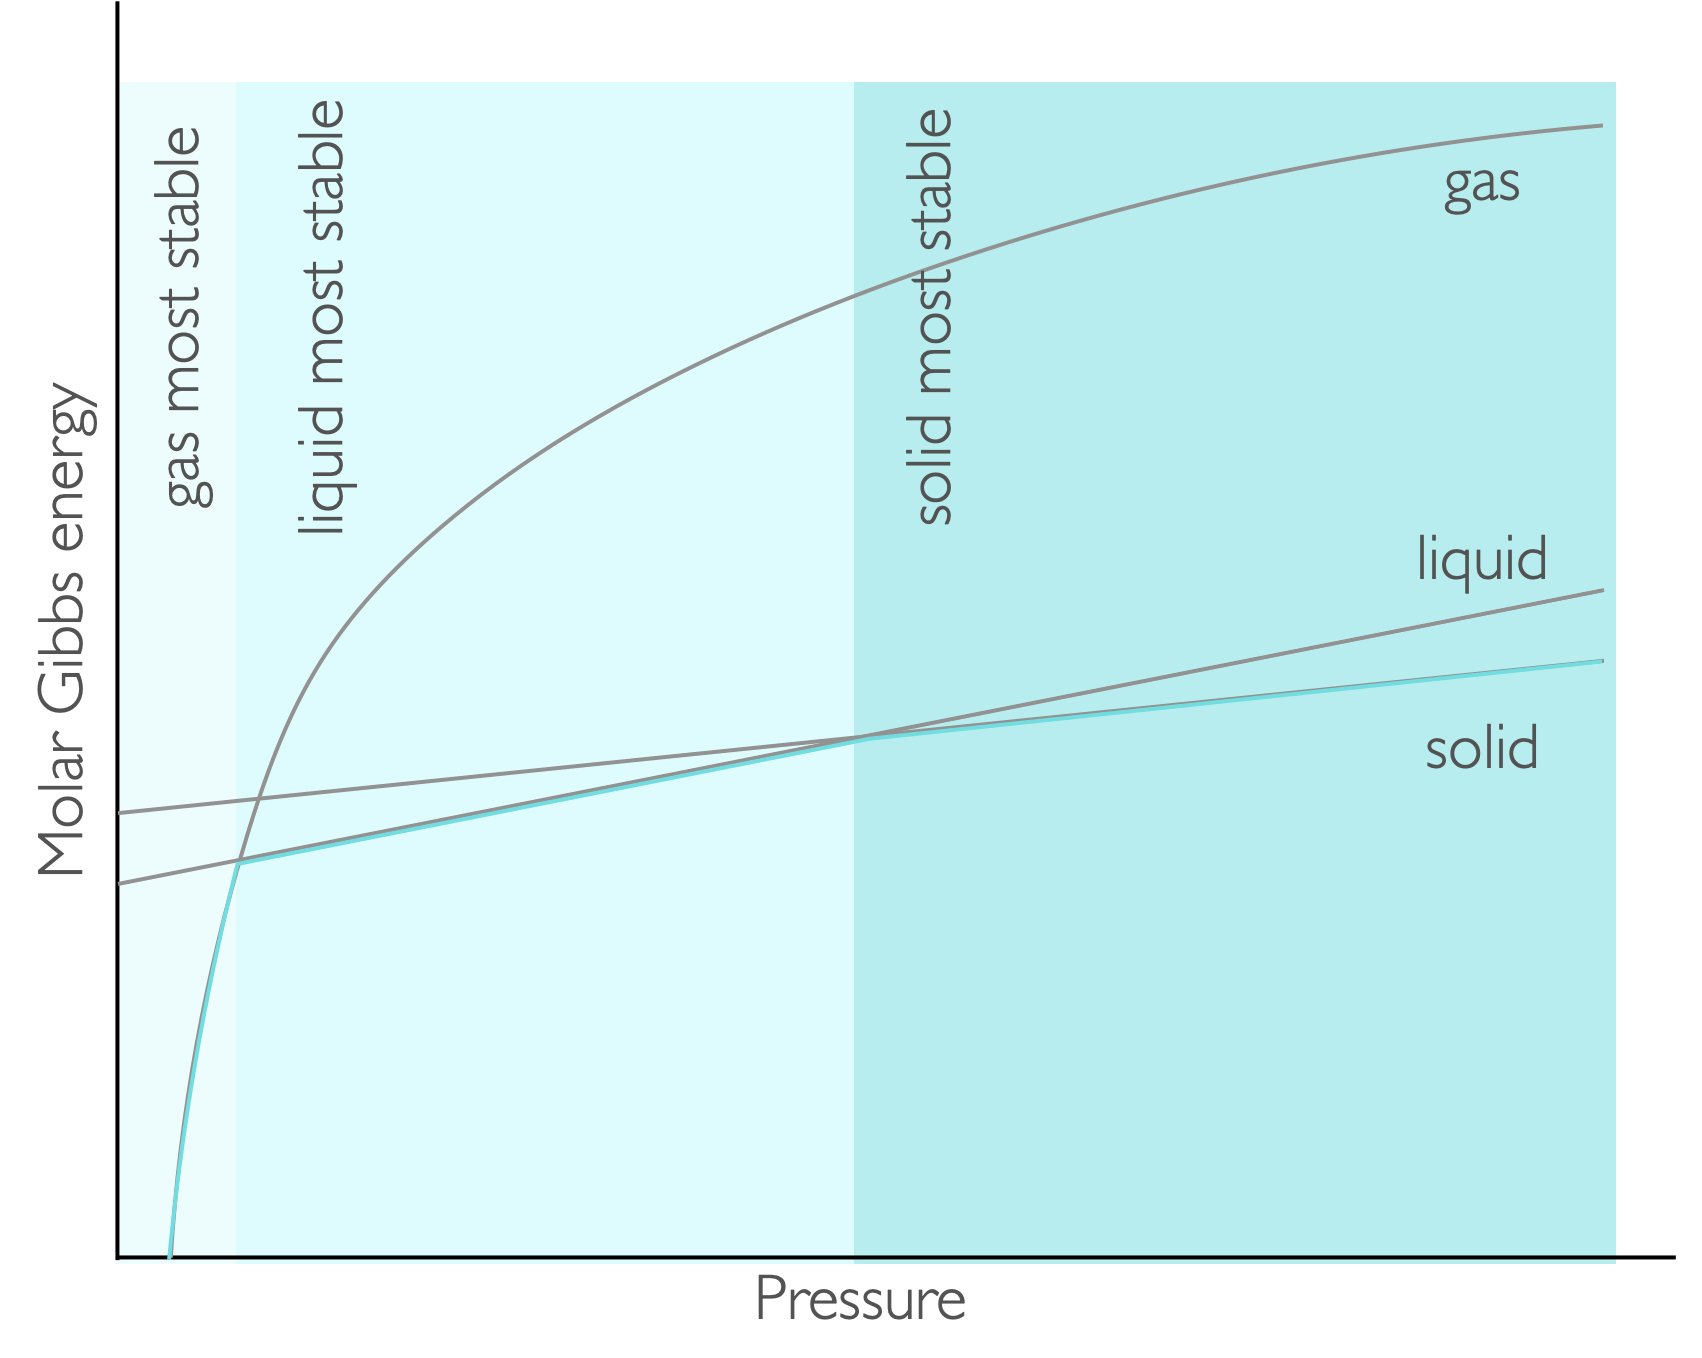
\includegraphics[width=0.8\linewidth]{images/gibbspressurestate} 

}

\caption{For pressure the molar Gibbs energy varies as a function of pressure with the gradient being the molar volume. At low pressures the gas is the most stable, with liquid and solid being favoured as the pressure increases.}\label{fig:gibbspressurestate}
\end{figure}

\hypertarget{clausius-clapeyron-equation}{%
\subsection{Clausius-Clapeyron equation}\label{clausius-clapeyron-equation}}

The Clausius-Clapeyron equation shows how the pressure and temperature are linked at the liquid gas phase boundary.

\begin{equation}
\ln \frac{p_2}{p_1}=-\frac{\Delta _{vap}H}{R}\left( \frac{1}{T_2}-\frac{1}{T_1}\right)
\label{eq:clausiusclapeyron}
\end{equation}

Here we can predict the temperature of boiling as the pressure changes if we know these values for the phase change at another temperature and pressure.

We know that the driving force of a reaction depends upon pressure, \(\Delta G _m = V_m \Delta p\), this means that we can determine the relative position of lines of a GT plot based upon the pressure and molar volumes of the two phases.

\begin{figure}

{\centering 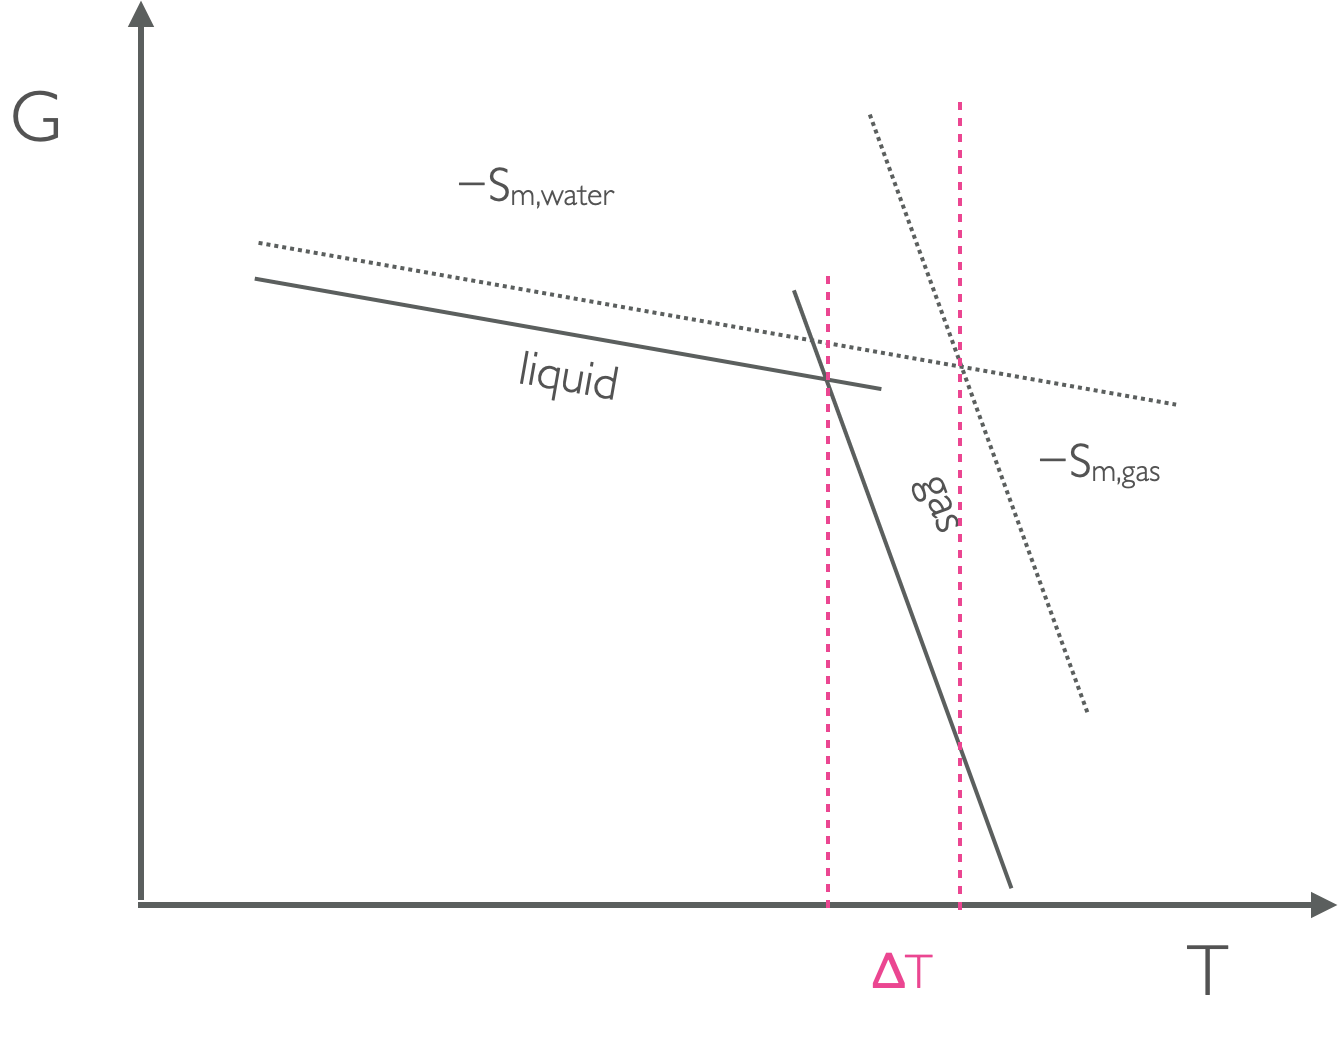
\includegraphics[width=0.8\linewidth]{images/boilingpressure} 

}

\caption{As the pressure changes the position of the lines on a GT plot move up or down depending on the molar volume, this means that at higher pressure the point where the lines from liquid and gas moves and the temperature of the phase change is different.}\label{fig:boilingpressure}
\end{figure}

\hypertarget{clapeyron-equation}{%
\subsection{Clapeyron equation}\label{clapeyron-equation}}

The Clapeyron equation shows how the pressure and temperature are linked at the solid liquid phase boundary:

\begin{equation}
\Delta p=\frac{\Delta_{fus} H}{T \Delta _{fus}V}\Delta T
\label{eq:clapeyron}
\end{equation}

Here the pressure and temperature are linked by the melting temperature, \(T\), enthalpy of fusion, \(\Delta _{fus}H\), and change in molar volume of the phase change \(\Delta _{fus} V\).

A similar plot to figure \ref{fig:boilingpressure} can be used to justify the difference in temperature of fusion with changing pressure.

It should be noted that the temperature difference of fusion at different pressures are much smaller than for equivalent temperatures and pressures for vaporisation.

\hypertarget{sec:w4p1question}{%
\section{Questions}\label{sec:w4p1question}}

\begin{enumerate}
\def\labelenumi{\arabic{enumi}.}
\item
  Calcium carbonate, CaCO\textsubscript{3}, decomposes to form CaO and CO\textsubscript{2} with ΔH = 178 kJ mol\textsuperscript{-1} and ΔS = 161 J K\textsuperscript{-1} mol\textsuperscript{-1}. Estimate the temperature at which the decomposition becomes spontaneous.
\item
  Calculate the melting temperature of benzene at exactly 100 bar. (\(\Delta _{fus} H\) = + 10.59 kJ mol\textsuperscript{-1}, \(T_m\) = 278.7 K, \(V_m\) (l)= 88.86 cm\textsuperscript{3} mol\textsuperscript{−1}, \(V_m\) (s)= 87.67 cm\textsuperscript{3} mol\textsuperscript{−1}).
\item
  The standard Gibbs energy for a reaction is -332.9 kJ mol\textsuperscript{−1} at 298 K and -339.5 kJ mol\textsuperscript{−1} at 500 K. Estimate the standard entropy change for the reaction. You may assume that H and S do not vary in this temperature range.
\item
  The saturated vapour pressure of a compound is 2.339 kPa at 20 °C and 19.948 kPa at 60 °C. Calculate the enthalpy change of vaporization.
\end{enumerate}

\hypertarget{sec:w4p1answer}{%
\section{Answers}\label{sec:w4p1answer}}

\begin{enumerate}
\def\labelenumi{\arabic{enumi}.}
\item
  T = 1.11 kK
\item
  T\textsubscript{fus} (100 bar) = 279.0 K
\item
  \(\Delta H\) = −323.2 kJ mol\textsuperscript{-1}
\item
  \(\Delta_{vap} H\) = 43.5 kJ mol\textsuperscript{-1}
\end{enumerate}

\hypertarget{ch:Part8}{%
\chapter{Week 4 - Part 2}\label{ch:Part8}}

\hypertarget{how-ux3b4g-relates-to-the-equilibrium-constant-k}{%
\section{How ΔG relates to the equilibrium constant, K}\label{how-ux3b4g-relates-to-the-equilibrium-constant-k}}

The driving force of a reaction, ΔG\textsubscript{⦵} , is linked to the equilibrium constant for that process by equation \eqref{eq:Gibbsequilibrium}.

\begin{equation}
\Delta G^\ominus = -RT \ln K
\label{eq:Gibbsequilibrium}
\end{equation}

Consequently, the bigger the driving force of a reaction ( the more negative ΔG\textsuperscript{⦵}) the more the equilibrium lies towards the products of a reaction. Here we introduce a second version of the Gibbs' free energy (ΔG), this is for when we are looking at the driving force of the reaction but for at any point in the reaction where we no longer have pure reactants and pure products.

\begin{figure}

{\centering 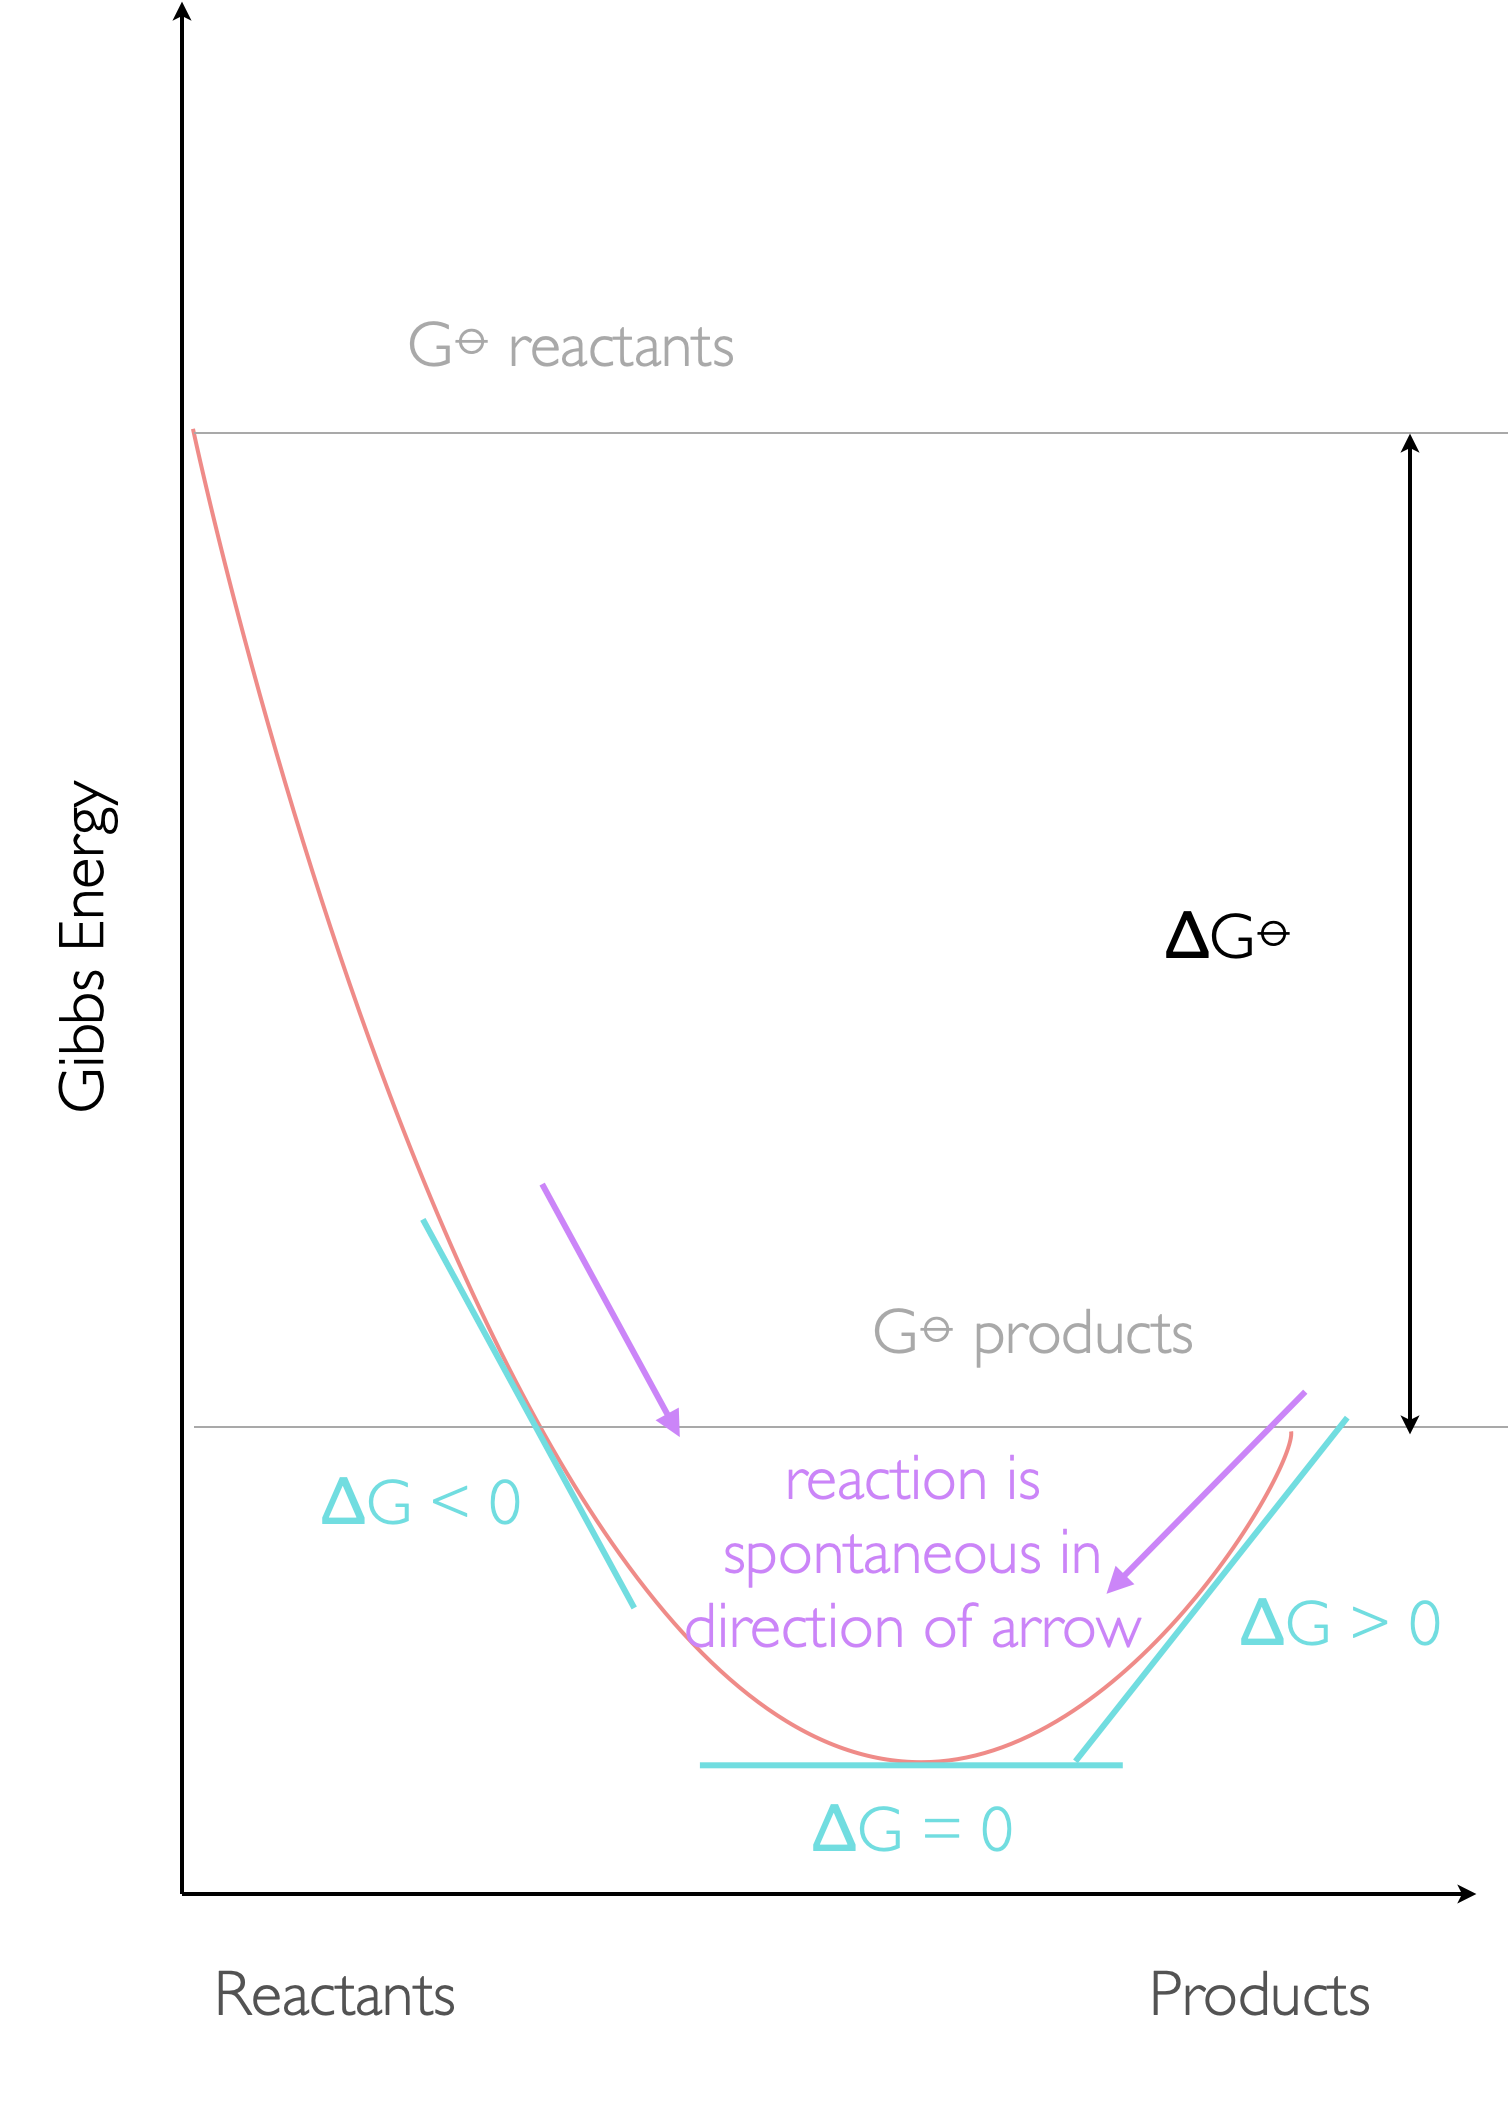
\includegraphics[width=0.5\linewidth]{images/gibbsequilibrium} 

}

\caption{The reaction profile showing the Gibbs free energy (ΔG⦵) between pure reactants and products but also the driving force (ΔG). at any point of the reaction, the equilibrium is reached when ΔG=0 and both forward and backward reactions will occur until the compositon of the system matches the position of the thermodynamic equilibrium.}\label{fig:gibbsequilibrium}
\end{figure}

If we look at this on a molecular level, we know that the population of energy levels depends upon temperature, and we have previously seen in equation \eqref{eq:Gibbs} that the Gibbs free energy also depends upon the enthalpy and entropy of the system. Enthalpy gives us the relative positions of the bottom or the ladder (or well) for reactants and products and entropy is related to the closeness of energy levels and the number of available microstates.

\begin{figure}

{\centering 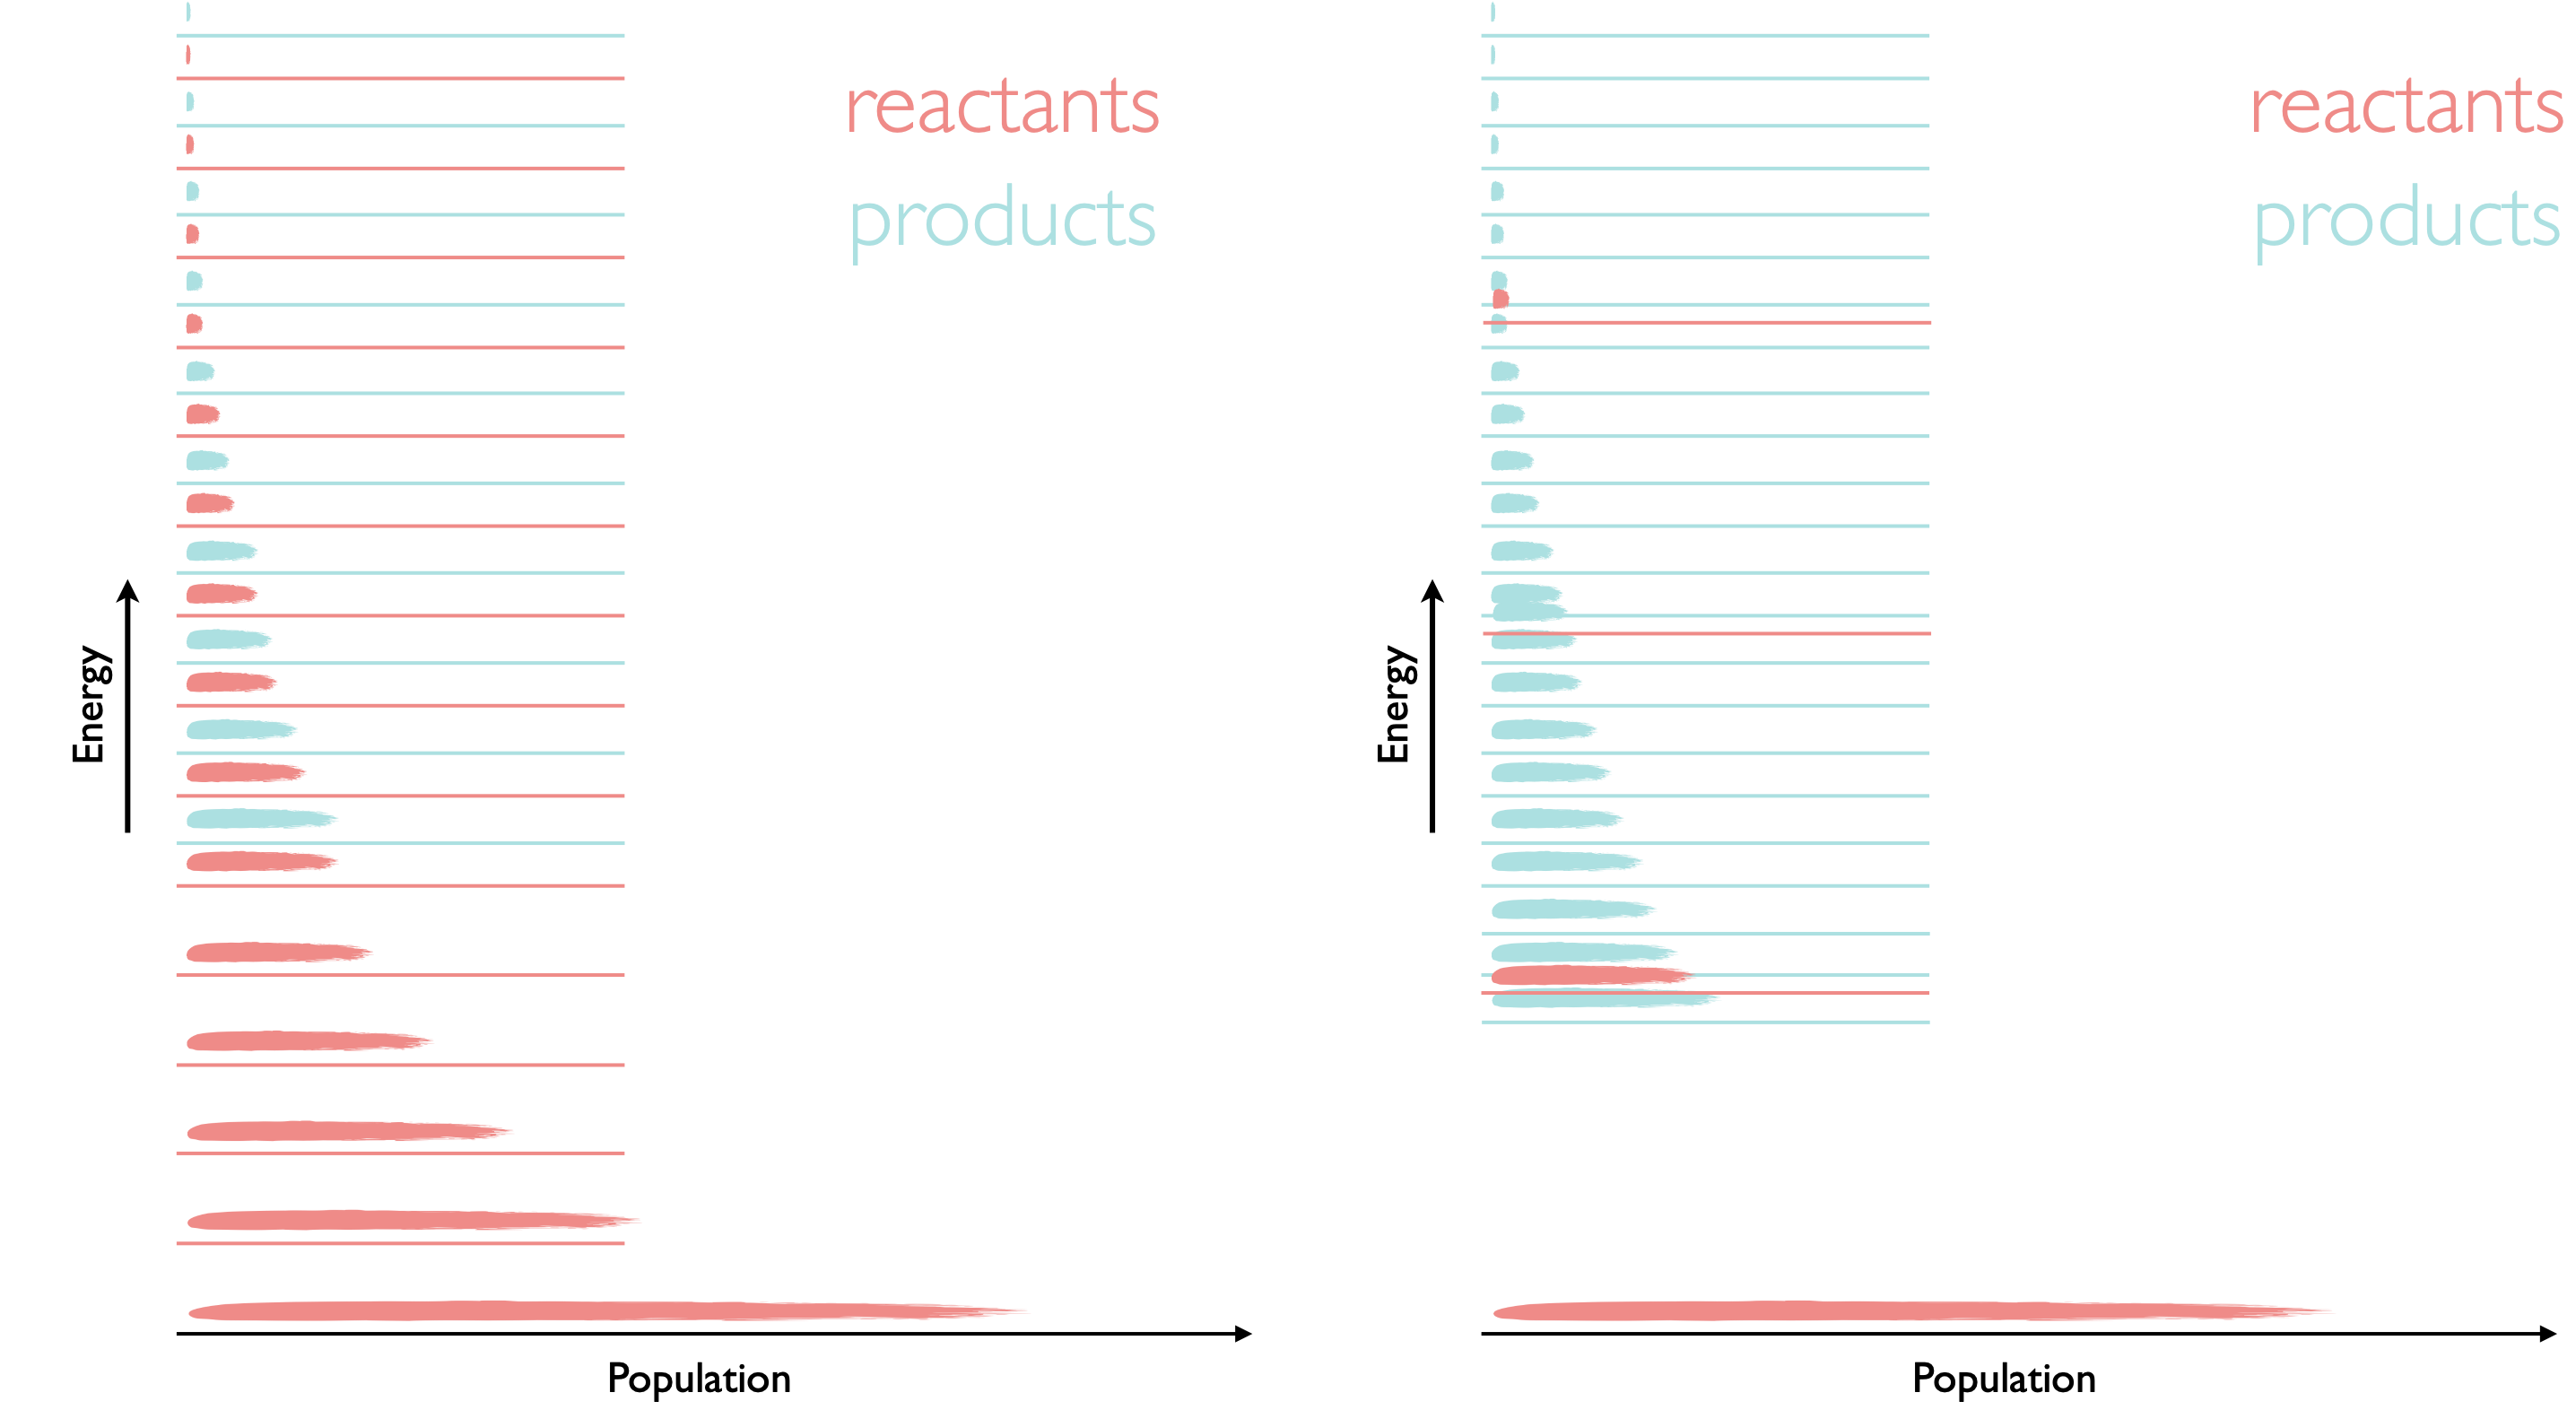
\includegraphics[width=1\linewidth]{images/energyleveleq} 

}

\caption{The two systems are both endothermic (ΔH⦵ is +ve) but for the case of the system on the left the entropy is similar for both reactants and products and therefore the equilibrium position (following a Boltzmann distribution across all available energy levels) favours the reactants. For the system on the right due to the closely packed energy levels more microstates are available for the products and so it has a higher entropy, conseqnently the product in this case is much more favoured.}\label{fig:energyleveleq}
\end{figure}

\hypertarget{the-equilibrium-constant-k}{%
\subsection{The equilibrium constant, K}\label{the-equilibrium-constant-k}}

The equilbrium constant for a reaction is defined as the \emph{activity} of the products raised to their stoichiometric quantity divided by the \emph{activity} of the reactants raised to their stoichiometric quantity (equation \eqref{eq:equilibrium}).

\begin{equation}
K = \frac{a_C^ca_D^d}{a_A^aa_B^b}
\label{eq:equilibrium}
\end{equation}

Activity is sometimes called the \emph{effective concentration} and so it makes sense that the thermodynamics depends upon activity and not concentration or pressure although equivalent expressions for concentration and pressure may be determined with equilibrium constants \(K_c\) and \(K_p\) respectively. However we cannot take the log of any value with units and so these versions of equilibrim constant are largely useless in thermodynamics.

For most gaseous systems at atmospheric pressure or lower ideality is a reasonable assumption, as is ideality of low concentration solutions of none charged species, however any ionic solution quickly deviates from ideality at very low concentration and so the activity coefficient needs to be calculated.

The activity of an dissolved species may be determined from:

\begin{equation*}
a_x = \gamma \frac{[X]}{[X]_0}= \gamma \frac{[X]}{1 \textrm{ mol dm}^{-3}}
\end{equation*}

and the activity of a gaseous species from the equivalent expression:

\begin{equation*}
a_x =\gamma \frac{p_x}{P_{x0}}= \gamma\frac{p_x}{1 \textrm{ bar}}
\end{equation*}

\hypertarget{le-chuxe2teliers-principle}{%
\subsection{le Châtelier's principle}\label{le-chuxe2teliers-principle}}

The whole point of an equilibrium is that the composiont of the system is defined by the equilbrium constant K, the only thing which affects K is the thermodyanamic temperature.

le Châtelier's principle states \emph{`if a change is made to a system in dynamic equilibrium the system will respond so as to oppose the change'}, so if we add more product to ensure the equilibrium is restored some product will undergo the back reaction to produce reactants such that the value of K is unchanged.

Another example could be for a gaseous reaction where if we increase the pressure of the system at equilibrium we disturb the equilibrium and the sytem will react to reduce (if possible) the total number of moles (or move to the side of the reaction with the lowest molar volume).

\hypertarget{effect-of-catalysts}{%
\subsection{Effect of catalysts}\label{effect-of-catalysts}}

Catalysts affect rate, not thermodyanamics, the presence of a catalyst will affect the rate of both forward and back reactions but the position of the equilibrium will be unchanged. (Reactions are always occuring, but at equilibrium the rate of the forward reaction and rate of back reaction are the same).

Catalysts affect the rate by affecting the height of the activation barrier, this is in effect lowering the Gibbs' free energy of the transition state (figure \ref{fig:catalyst}).

\begin{figure}

{\centering 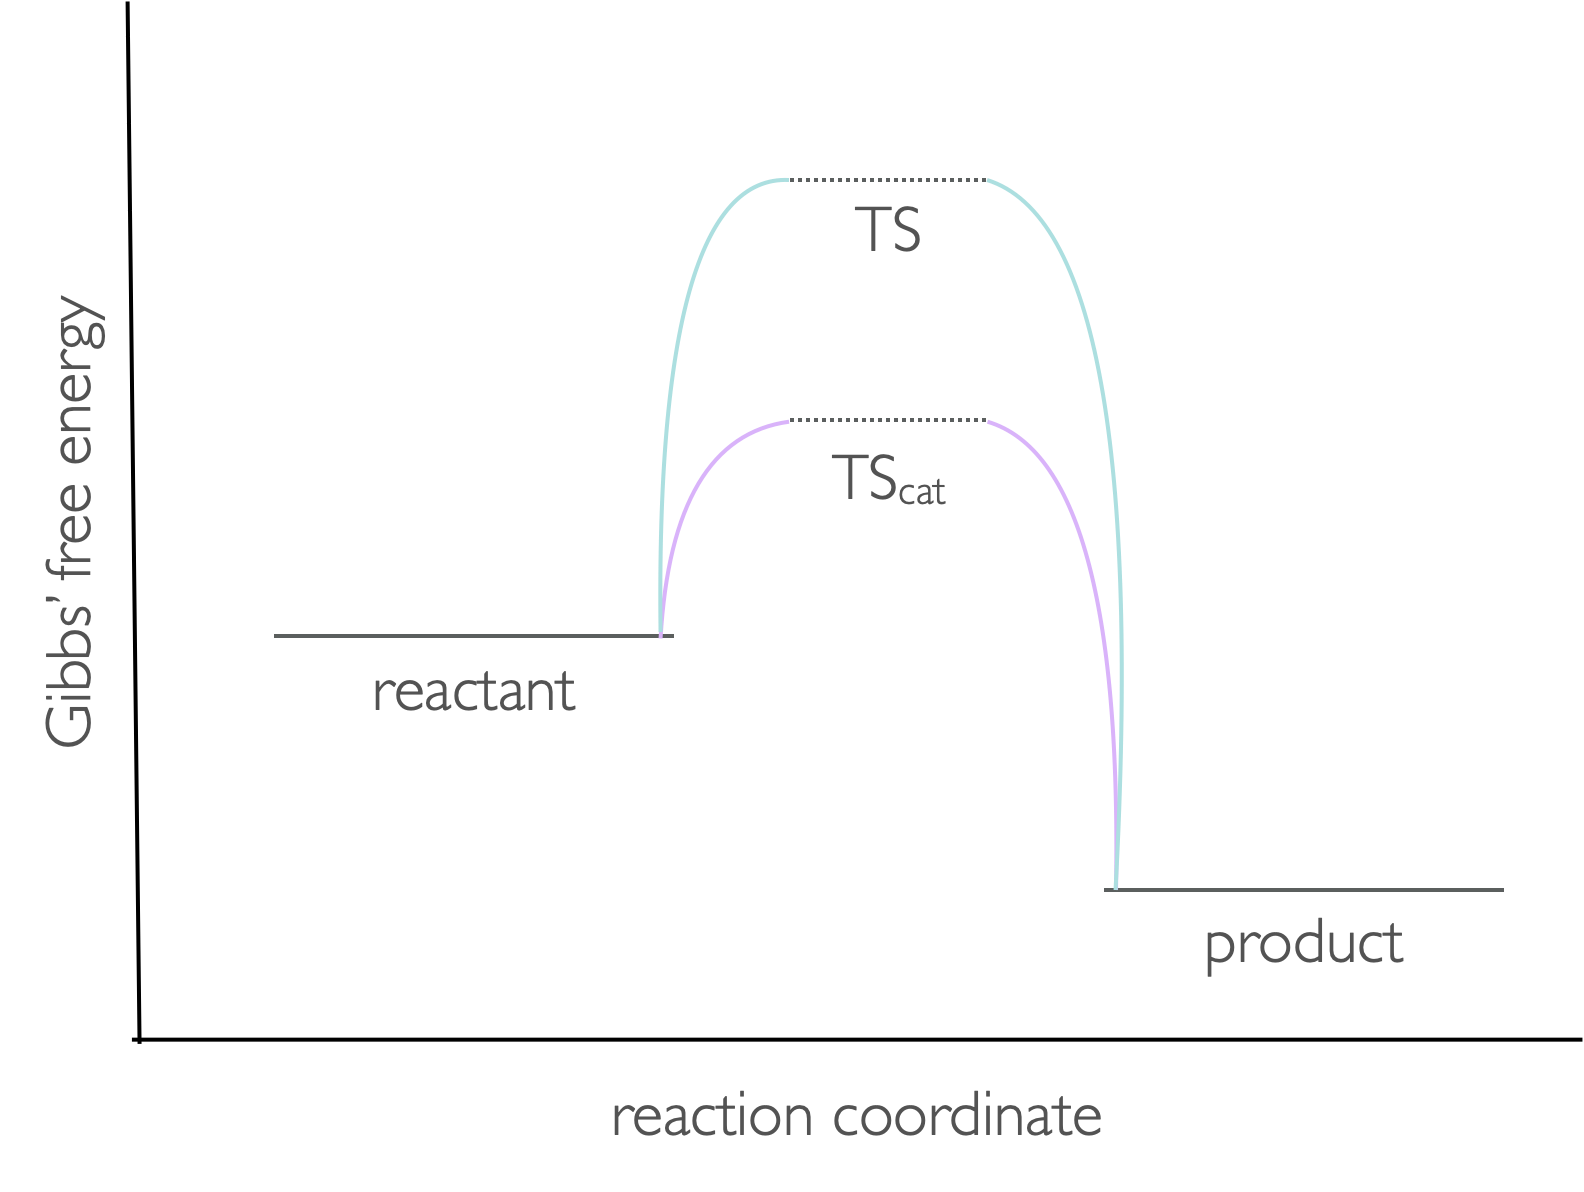
\includegraphics[width=1\linewidth]{images/catalyst} 

}

\caption{The transition state during a reaction has a higher Gibbs free energy than either the reactants or products. The presence of a catalyst lowers the energy of this transition state.}\label{fig:catalyst}
\end{figure}

\hypertarget{sec:quotient}{%
\section{Reaction quotient}\label{sec:quotient}}

We can define the reaction quotient, Q, at any point during a reaction:

\begin{equation}
Q = \frac{a_C^ca_D^d}{a_A^aa_B^b}
\label{eq:quotient}
\end{equation}

The expression for reaction quotient is the same used as for equilibrium constant but is true for any values of activity of reactants and products. This means that we can determine the driving force (or remaining work we can derive from a reaction) at any point in the reaction, not just for pure reactants and products.

\begin{equation}
\Delta _r G = \Delta _r G ^ \ominus + RT \ln Q
\label{eq:gibbsquotient}
\end{equation}

\hypertarget{sec:tempK}{%
\section{How temperature affects K}\label{sec:tempK}}

We have already seen that both the enthalpy and entropy (and therefore Gibbs' free energy) depend upon temperature, and we have also seen that the equilibrium composition (and therefore equilibrium constant) also depends upon tempearture.

Henry van't Hoff combined two expressions for Gibbs' free energy (equations \eqref{eq:Gibbsequilibrium} and \eqref{eq:Gibbs}) to give the van't Hoff equation:

\begin{equation}
\ln K = -\frac{\Delta_r H^\ominus }{R}\frac{1}{T}+ \frac{\Delta_r S^\ominus }{R}
\label{eq:vanthoff}
\end{equation}

\begin{figure}

{\centering 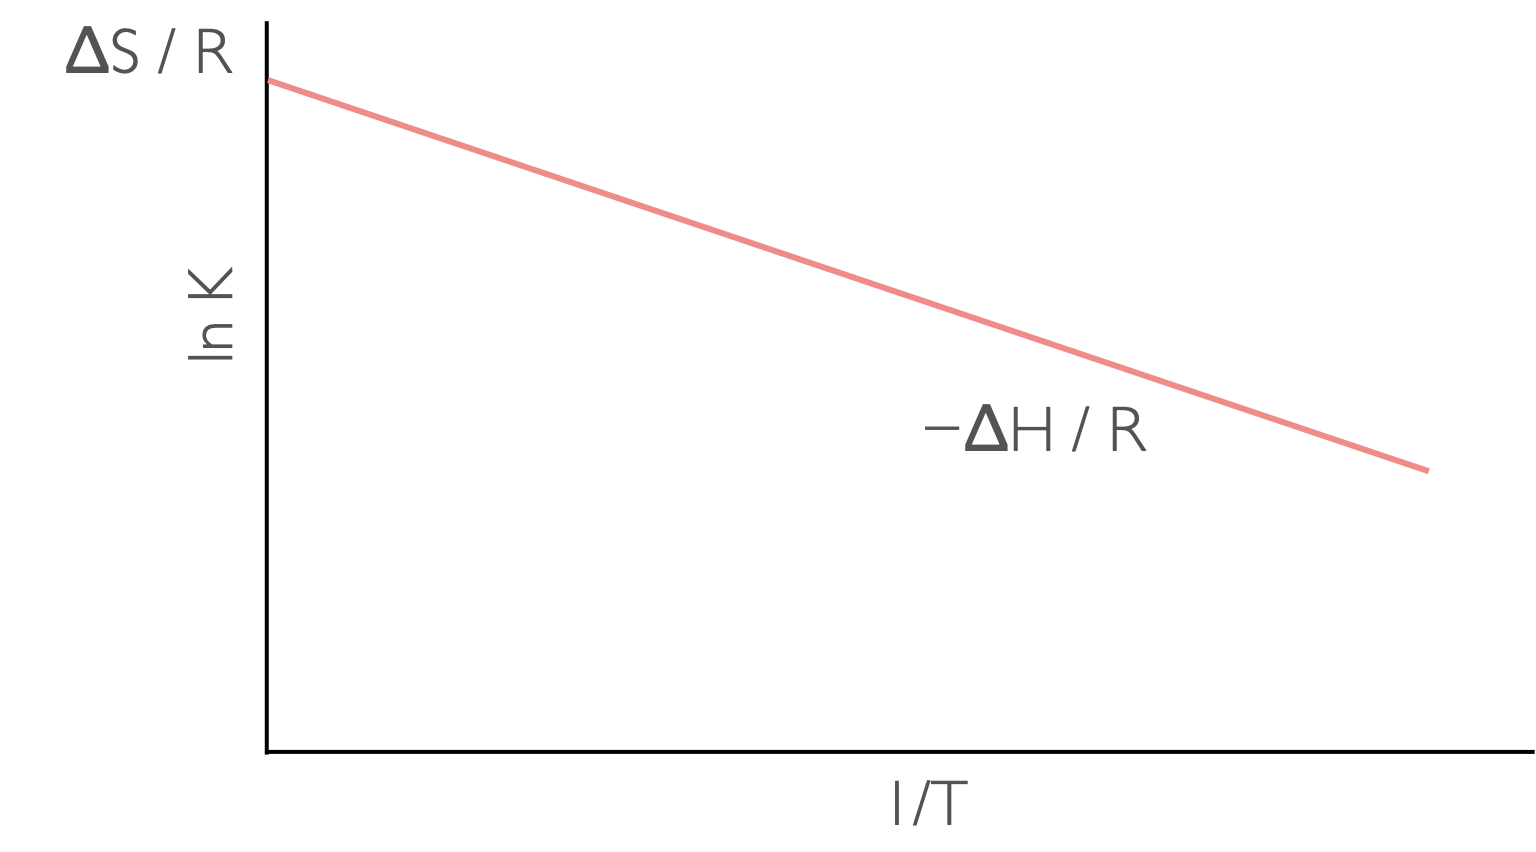
\includegraphics[width=1\linewidth]{images/vanthoff} 

}

\caption{A plot of ln K against 1/T  has a gradient of −ΔH/R and an intercept of ΔS (assuming ΔH and ΔS are linear over the range studied.}\label{fig:vanthoff}
\end{figure}

\hypertarget{third-law-for-completeness}{%
\section{Third Law (for completeness)}\label{third-law-for-completeness}}

The third law, unlike the first three laws (the zeroth - which introduced temperature), the first (internal energy) and the second (entropy) doesn't introduce a new thermodynamic concept. Instead it extends our understanding of both entropy and internal energy.

\emph{the entropy of all perfectly crystalline substances is zero at zero kelvin}

Another way of stating the third law is that no body may be cooled to absolute zero\ldots{} some people have got close cooling samples to 10\textsuperscript{−12} K. One of the problems is at very low temperatures heat capacities are also very, very low; consequently small inputs of `heat' lead to large increases of the temperature of very cold systems.

\begin{figure}

{\centering 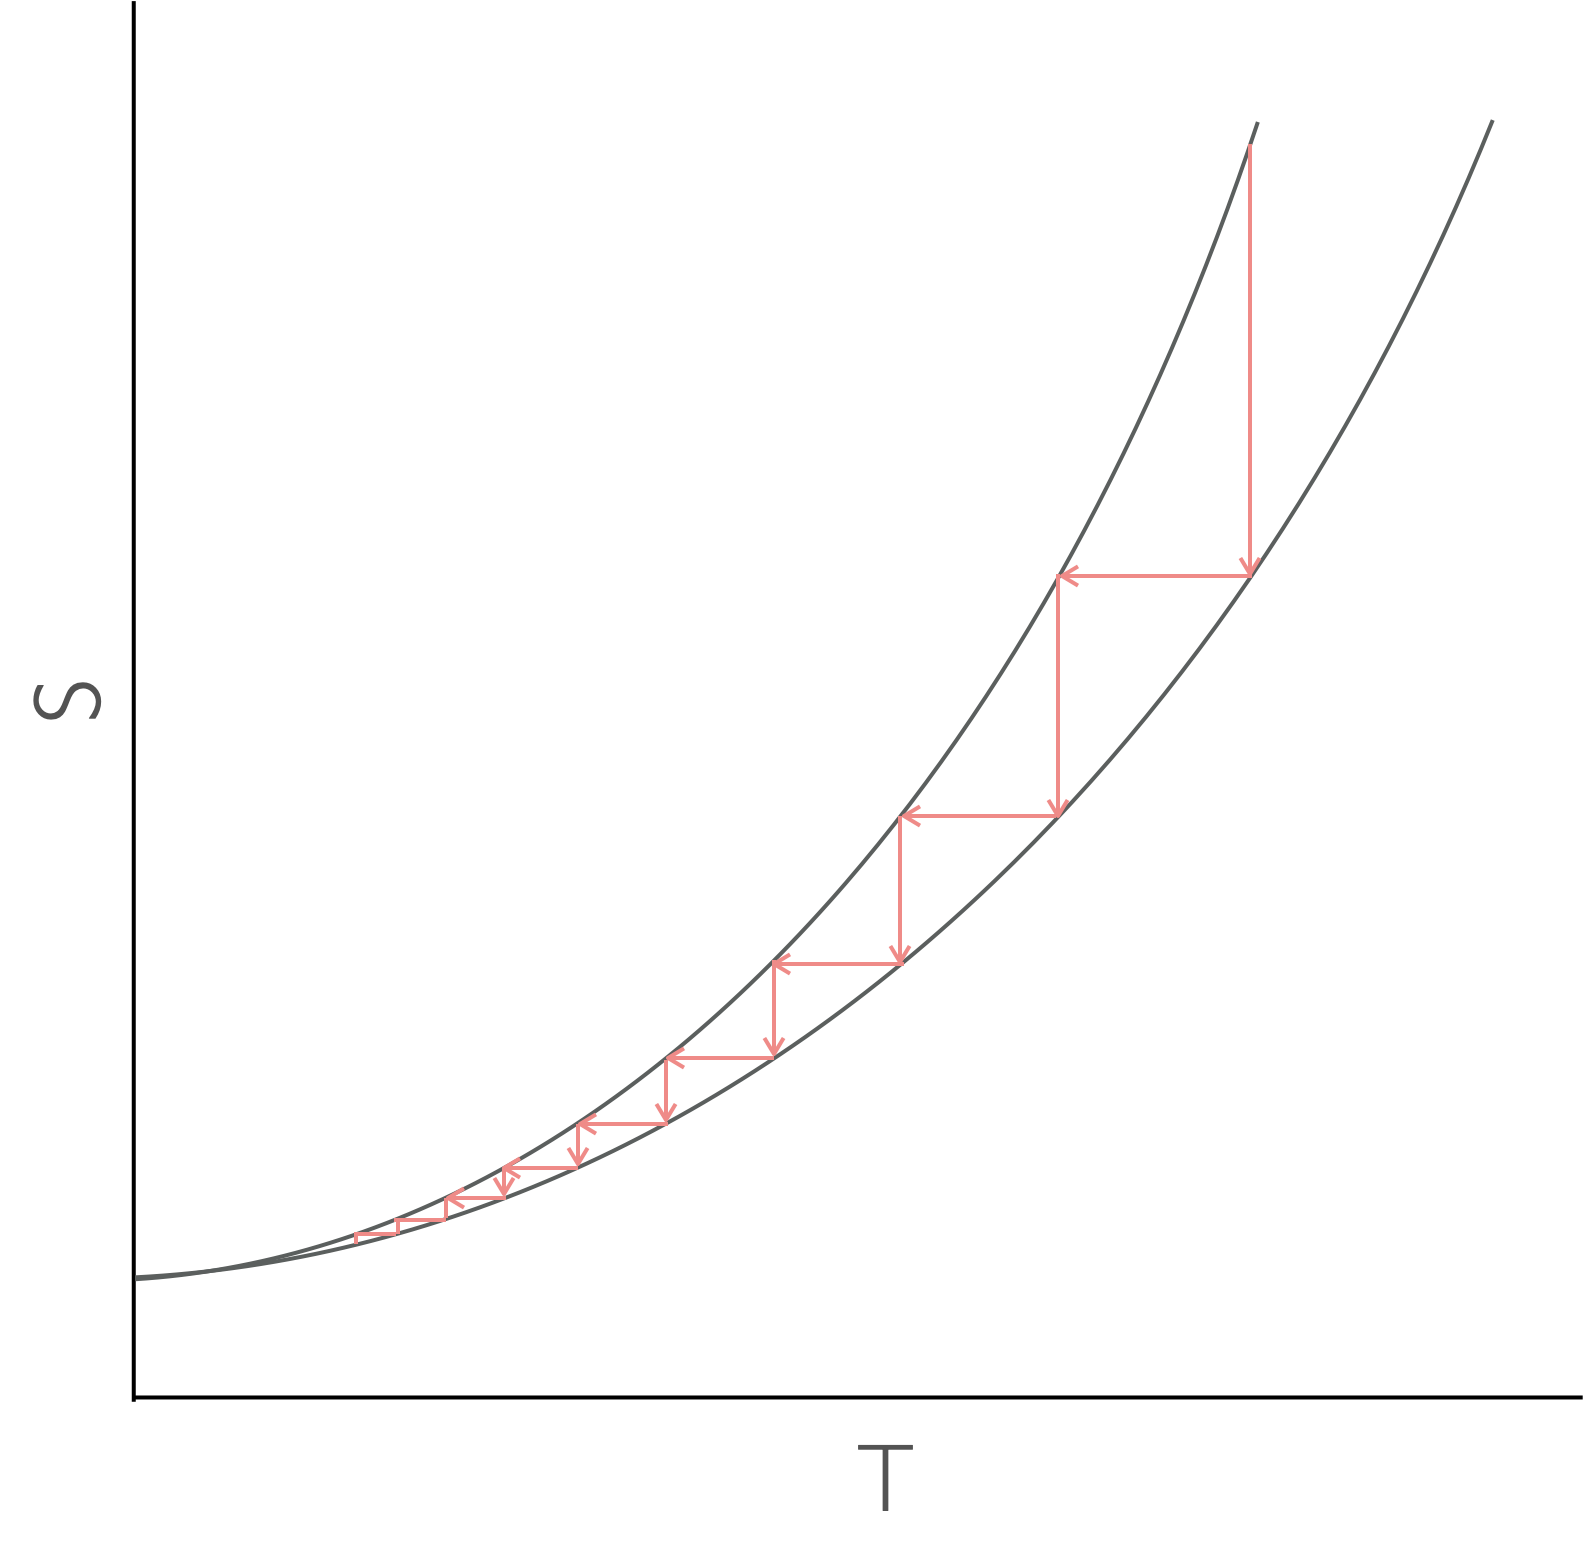
\includegraphics[width=1\linewidth]{images/cooling} 

}

\caption{As a two state system is cooled the entropy of the two states converges at absolute zero. There is no way to cool to zero by successively lowering the entropy then temperature, you just itterate every closer.}\label{fig:cooling}
\end{figure}

\hypertarget{sec:w4p2question}{%
\section{Questions}\label{sec:w4p2question}}

\begin{enumerate}
\def\labelenumi{\arabic{enumi}.}
\item
  Write the expression for the equilibrium constant K for the following reaction.
  4 NH\textsubscript{3} (g) + 7 O\textsubscript{2} (g) \(\leftrightharpoons\) 4 NO\textsubscript{2} (g) + 6 H\textsubscript{2}O (l)
\item
  N\textsubscript{2}O\textsubscript{4} \(\leftrightharpoons\) 2 NO\textsubscript{2}
\end{enumerate}

\begin{enumerate}
\def\labelenumi{\alph{enumi}.}
\item
  If the equilibrium constant for the above reaction is 3.89 \(\times 10^5\) at \(75 ^{\circ}\)C and 4.79 \(\times 10^6\) at \(125 ^{\circ}\)C what is the enthalpy of the reaction?
\item
  What assumptions have you made?
\item
  What partial pressure of product would you expect if 0.500 bar of reactant reaches equilibrium at 298 K?\textbackslash{}
\end{enumerate}

\begin{enumerate}
\def\labelenumi{\arabic{enumi}.}
\setcounter{enumi}{2}
\tightlist
\item
  Silver carbonate decomposes on heating. Calculate the equilibrium constant at 110°C for the reaction:
\end{enumerate}

Ag\textsubscript{2}CO\textsubscript{3} (s) \(\leftrightharpoons\) Ag\textsubscript{2}O + CO\textsubscript{2}

\begin{longtable}[]{@{}cccc@{}}
\toprule
& Ag\textsubscript{2}CO\textsubscript{3} & Ag\textsubscript{2}O & CO\textsubscript{2}\tabularnewline
\midrule
\endhead
ΔH\textsuperscript{⦵} / kJ mol\textsuperscript{−1} & −501.4 & −29.07 & −393.5\tabularnewline
S\textsubscript{m}\textsuperscript{⦵} / J K\textsuperscript{−1} mol\textsuperscript{−1} & 167.3 & 121.7 & 213.7\tabularnewline
C\textsubscript{p} / J K\textsuperscript{−1} mol\textsuperscript{−1} & 109.6 & 68.6 & 37.1\tabularnewline
\bottomrule
\end{longtable}

\hypertarget{sec:w4p2answer}{%
\section{Answers}\label{sec:w4p2answer}}

\begin{enumerate}
\def\labelenumi{\arabic{enumi}.}
\item
  \(K = \frac{a_{NO_2}^4 a_{H_2O}^6}{a_{NH_3}^4 a_{O_2}^7}\)
\item
  \begin{enumerate}
  \def\labelenumii{\alph{enumii}.}
  \tightlist
  \item
    Δ\textsubscript{r}H\textsuperscript{⦵} = +57.8 kJ mol\textsuperscript{−1}
  \item
    Δ\textsubscript{r}H\textsuperscript{⦵} is constant over the temperature range
  \item
    p(NO\textsubscript{2}) = 1.00 bar (the reaction goes to near completion)
  \end{enumerate}
\item
  K = 0.01053
\end{enumerate}

\hypertarget{additional-questions}{%
\chapter{Additional questions}\label{additional-questions}}

It is always important to learn how to solve questions out of the original context of the material taught. After completing this course you should now be able to answer any of these questions.

\hypertarget{questions-3}{%
\section{Questions}\label{questions-3}}

\begin{enumerate}
\def\labelenumi{\arabic{enumi}.}
\item
  Calculate the entropy change when 2.50 mol of mercury vaporises at its boiling point of 356.55 ºC. Δ\textsubscript{vap}H\textsuperscript{⦵} = + 59.229 kJ mol\textsuperscript{−1}.
\item
  Calculate the free energy change at 25 ºC and 250 ºC for the following reaction:
\end{enumerate}

MgO (s) + CO (g) ⟶ Mg (s) + CO\textsubscript{2} (g)

\begin{longtable}[]{@{}cccc@{}}
\toprule
& Δ\textsubscript{f}H\textsuperscript{⦵} & S\textsuperscript{⦵}\textsubscript{m} J K\textsuperscript{−1} mol\textsuperscript{−1} & C\textsubscript{p} / J K\textsuperscript{−1} mol\textsuperscript{−1}\tabularnewline
\midrule
\endhead
MgO (s) & -601.7 & 26.9 & 37.2\tabularnewline
CO (g) & -110.5 & 197.7 & 29.1\tabularnewline
Mg (s) & 0 & 32.7 & 24.9\tabularnewline
CO\textsubscript{2} (g) & -393.5 & 213.7 & 37.1\tabularnewline
\bottomrule
\end{longtable}

State what assumptions you have made.

\begin{enumerate}
\def\labelenumi{\arabic{enumi}.}
\setcounter{enumi}{2}
\tightlist
\item
  For the reaction:
\end{enumerate}

A + B ⇌ 2C

Determine the equilibrium concentration of C if the Gibbs energy for the reaction at 20 ºC is −40.0 kJ mol\textsuperscript{−1} and at equilibrium the concentration of A is 0.0500 mol dm\textsuperscript{−3} and B is 0.0450 mol dm\textsuperscript{−3}.

\begin{enumerate}
\def\labelenumi{\arabic{enumi}.}
\setcounter{enumi}{3}
\tightlist
\item
  The Clausius-Clapeyron equation can be used to determine the enthalpy of vaporisation:
\end{enumerate}

\begin{equation*}
\ln p = -\frac{Delta _{\textrm{vap}}H}{RT}+C
\end{equation*}

Given the data for ethyl acetate (Table \ref{tab:ethylacetatedata}), determine the enthalpy of vaporization of ethyl acetate, and consequently determine the boiling point (at 1 bar).

\begin{longtable}[]{@{}cc@{}}
\caption{\label{tab:ethylacetatedata} The equilibrium vapour pressure of ethyl acetate at differing temperatures.}\tabularnewline
\toprule
T / ºC & p / 10\textsuperscript{3} Pa\tabularnewline
\midrule
\endfirsthead
\toprule
T / ºC & p / 10\textsuperscript{3} Pa\tabularnewline
\midrule
\endhead
9.1 & 5.304\tabularnewline
27.4 & 13.33\tabularnewline
59.3 & 53.31\tabularnewline
77.1 & 101.32\tabularnewline
100.6 & 202.6\tabularnewline
136.6 & 506.7\tabularnewline
\bottomrule
\end{longtable}

\begin{enumerate}
\def\labelenumi{\arabic{enumi}.}
\setcounter{enumi}{4}
\tightlist
\item
  Determine the equilibrium constant for the following reaction at 150 oC,
  :::centre
  N\textsubscript{2}O\textsubscript{5} (g) ⟶ NO\textsubscript{2} (g) + NO (g) + O\textsubscript{2} (g)
  :::
\end{enumerate}

\begin{longtable}[]{@{}cccc@{}}
\toprule
& Δ\textsubscript{f}H\textsuperscript{⦵} & S\textsuperscript{⦵}\textsubscript{m} J K\textsuperscript{−1} mol\textsuperscript{−1} & C\textsubscript{p} / J K\textsuperscript{−1} mol\textsuperscript{−1}\tabularnewline
\midrule
\endhead
NO (g) & +90.25 & 210.76 & 29.844\tabularnewline
NO\textsubscript{2} (g) & +33.18 & 240.06 & 37.20\tabularnewline
N\textsubscript{2}O\textsubscript{5} (g) & +11.3 & 355.7 & 84.5\tabularnewline
O\textsubscript{2} & - & 205.138 & 29.355\tabularnewline
\bottomrule
\end{longtable}

\hypertarget{answers-2}{%
\section{Answers}\label{answers-2}}

\begin{enumerate}
\def\labelenumi{\arabic{enumi}.}
\item
  235 J K\textsuperscript{-1}
\item
  ΔG\textsubscript{298} = +318.7 kJ mol\textsuperscript{-1}, ΔG\textsubscript{523} = 307.6 kJ mol\textsuperscript{-1}
\item
  {[}C{]} = 174 mol dm\textsuperscript{-1} (so big it is essentially all product!)
\item
  Δ\textsubscript{vap}H = +34.5 kJ mol\textsuperscript{-1}, T\textsubscript{b} = 78 ºC
\item
  K = 3.649 × 10\textsuperscript{29}
\end{enumerate}

\hypertarget{glossary-of-terms}{%
\chapter*{Glossary of terms}\label{glossary-of-terms}}
\addcontentsline{toc}{chapter}{Glossary of terms}

\hypertarget{a-f}{%
\section*{A-F}\label{a-f}}
\addcontentsline{toc}{section}{A-F}

\begin{itemize}
\item
  Adiabatic system: An adiabatic system can have no exchange of matter, and energy can only be exchanged in the form of work between the system and surroundings
\item
  Closed system: A closed system is one where there can be no exchnage of matter, but energy in either the form of heat or work may be exchanged between the system and surroundings.
\item
  Endothermic: an endothermic reaction has a positive value for ΔH and energy is transferred from the surroundings to the system in the form of heat
\item
  Exothermic: an exothermic reaction has a negative value for ΔH and energy is transferred from the system to the surroundings in the form of heat
\item
  Extensive property: a property which is dependent upon the amount of `stuff' you have, such as mass, volume, and enthalpy.
\end{itemize}

\hypertarget{g-m}{%
\section*{G-M}\label{g-m}}
\addcontentsline{toc}{section}{G-M}

-Gibbs' free energy (G): the amount of non expansion work which can be derived from a system, if the value of Gibbs free energy change for a process is negative the reaction is spontaneous.

\begin{itemize}
\item
  Heat: a mode of transfer of energy which causes chaotic (or non-uniform) motion of the system or surroundings
\item
  Heat capacity: see specific heat capacity or molar heat capacity
\item
  Intensive property: a property which is independent of the amount of `stuff' you have, such as temperature, molar volume, and molar enthalpy.
\item
  Isobaric: at constant pressure.
\item
  Isochoric: at constant thermal.
\item
  Isolated system: An isolated system is one where there can be no exchange of either matter or energy between the system and surroundings
\item
  Isothermal: at constant temperature.
\item
  Macrostate: the overall way a system looks, a macrostate often has multiple ways (microstates) to achieve this state .
\item
  Microstate: the way a system looks as if we can uniquely identify individual particles.
\item
  Molar heat capacity: the energy in the form of heat requred to raise the temperature of 1 mol of a substance by 1 K
\end{itemize}

\hypertarget{n-s}{%
\section*{N-S}\label{n-s}}
\addcontentsline{toc}{section}{N-S}

\begin{itemize}
\item
  Open system: In an open system both matter and energy may be exchanged between the system and surroundings.
\item
  Path function: a path function is one which depends upon the route taken to go between the initial and final states. Functions such as work are path functions.
\item
  reversible: when a process is reversible in thermodynamics it is in equilibrium at all times and any changes which occur are infinitessimally small.
\item
  Specific heat capacity: the energy in the form of heat requred to raise the temperature of 1 kg (or 1 g) of a substance by 1 K
\item
  State function: a state function is one where only the current state of the system matters, for functions such as enthalpy change we only need to know the initial and final states and not how it got between those states.
\end{itemize}

\hypertarget{t-z}{%
\section*{T-Z}\label{t-z}}
\addcontentsline{toc}{section}{T-Z}

\begin{itemize}
\tightlist
\item
  Work: a mode of transfer of energy which causes uniform motion of the system or surroundings
\end{itemize}

  \bibliography{book.bib,packages.bib}

\end{document}
